\documentclass[12pt]{article}

% Set page size and margins
\usepackage[letterpaper,top=1in,bottom=1in,left=1in,right=1in]{geometry}

% Set line spacing
\renewcommand{\baselinestretch}{1.2}  % line spacing throughout document
\setlength{\skip\footins}{2em} % space between text and footnote
\newcommand{\floor}[1]{\left\lfloor #1 \right\rfloor}

% Useful packages
\usepackage{lipsum} % to generate filler text to help visualize formatting
\usepackage{amsmath}  % for math
\usepackage{graphicx} % for including figures
\usepackage{booktabs} % for nice-looking tables
\usepackage{caption}
\usepackage{subcaption}
\usepackage{breqn}
\usepackage[colorlinks=true, allcolors=blue]{hyperref} % for hyperlinks/references
\usepackage[skip=1.em]{parskip}  % leave vertical space between paragraphs
\usepackage{natbib}  % for bibliography
   \bibpunct{(}{)}{;}{a}{}{,}  % remove comma b/t author and year in citations to match ASA style
\usepackage{titlesec} % to adjust heading styles
    \titlelabel{\thetitle.\quad}  % add period after section number
\usepackage{float}
\usepackage[format=plain,
            labelfont={bf,it},
            textfont={it,small}]{caption}

% Adjusting abstract format
\renewenvironment{quote}
    {\small\list{}{\rightmargin=.5cm \leftmargin=.5cm}% change margins
    \item\relax}
    {\endlist}
\renewenvironment{abstract} 
    {\begin{quote}
    \noindent \rule{\linewidth}{.5pt}\par{\bfseries \abstractname.}}
    {\newline\medskip\noindent \rule{\linewidth}{.5pt}
    \end{quote}
    }


\begin{document}  % ----------------------------------------------------------------------------

% Heading
\title{\textbf{The Gerber Method} \\[6pt] \large Using Multipliers for Daily Box Office Prediction}

\author{\textbf{Aidan Gerber}}

\date{\today}  % you can change this if you want a specific date to print

\maketitle
\thispagestyle{empty}


% Abstract
\begin{abstract}
The movie industry is important to the United States both culturally and financially. A core part of the movie industry is exhibition at the domestic box office. 
This paper proposes and implements a model to predict the daily box office gross of a film over the entire course of its time in theaters. 
Using a novel approach based on daily, weekly, and seasonal multipliers, the model creates a robust time series which it updates as new data becomes available. To do this, comparison movies are found using a K-nearest neighbors model; then the individual characteristics of these similar movies are combined with a set of predicted multipliers.
The model is trained on a dataset of over 3,000 movies and their box office grosses from 2015 to 2025. 
This approach is not only novel, but the daily time series modeling is something no other paper has attempted.
Overall, we find very strong results with a median weighted mean absolute percentage difference (WMAPD) of 0.2.
\end{abstract}

\newpage


% Body of paper
\section{Introduction} \label{sec:intro}
% 1. Introduction: What’s the context? What have people already done? What will you do?
% (a) This section essentially combines your background, literature review, and research objective from your proposal. HOWEVER, you should not simply copy and paste those proposal sections here and call it done. Select the relevant pieces to keep, synthesize, add things in where necessary, and make sure things flow nicely.
% (b) You must have at least eight references in this section, including at least five academic journal articles. All references should be worked into the body of the paper, as opposed to listed in bullet points. Include commentary to make it clear how/why cited work relevant to your project, but you do not need complete summaries of the cited work.
% (c) This section should be at least a page long.
% (d) Refer back to the proposal guidelines for more on the flow (e.g., start by orienting the reader, go from broad to specific, define special terms, avoid unnecessary complexity,
% etc.).
% (e) Your introduction should end with a “roadmap” of the remaining sections. For example, “The remainder of this paper is organized as follows: In Section 2, we describe our two data sources. In Section 3, we detail the analysis methodology. In Section 4 we present our modeling results, and we conclude with a discussion in Section 5.”

% start with explaining the research space
Every year, Americans and Canadians spend billions of dollars watching movies in theaters. This is the domestic box office, which is the total revenue generated by movie theaters from ticket sales in the United States, Canada, and their territories \citep{numbersGlossary}. The domestic box office is a core part of the movie industry.

Box office grosses are a critical component of film profitability \citep{varietyOpeningWeekend}. There are also auxiliary revenue streams such as merchandise \citep{dunePopcorn}, premium video on demand \citep{wickedPvod}, streaming rights \citep{sonyNetflix}, and international box office \citep{dceuProfit}. However, domestic box office is one of the largest, most well-reported, and most transparently-published revenue streams for films. Studios report domestic box office figures daily to industry outlets such as \cite{deadlineHome}, \cite{hollywoodReporterHome}, and \cite{varietyHome}. These figures are also published by \cite{numbersHome} and \cite{bomHome}.

Since the domestic box office is such a large industry — totaling 8.6 billion dollars in 2024 and peaking at 11.9 billion dollars in 2018 — modeling it is important \citep{bomYearly}.

Accurate box office predictions have many possible use cases: theater owners looking to decide how many screens to dedicate to a movie, studios figuring out what productions to green-light and the most profitable release dates, investors looking to buy or sell stock in a studio, gamblers hoping to place accurate bets on box office performance, and simply hobbyists who love the game.

% do some literature review but explain the gaps
Most of the existing literature on box office predictions can be categorized as either (1) applying a model or (2) testing if a specific factor influences the box office. For example, \cite{dailyNeuralNetwork} apply the Deep-DBP algorithm, \cite{deeplearning} utilize a deep learning model, and 
\cite{svm} use support vector machines. As we seek to expand on these papers, we use a large dataset and focus on modeling every individual day of box office instead of just a few days, total gross, or categorization.
For specific factors, \cite{socialNetworkService} looks at social network popularity data, \cite{assessingBoxOffice} use movie scripts, \cite{modelingLifeCycles} highlight market share instead of absolute figures, and \cite{reviewsForetell} use natural language processing on reviews.

Additionally, there is a lack of literature for the post-COVID domestic box office period. COVID-19 caused a large shift in the overall box office, with theater revenue plummeting. Despite the recovery, 2024 still lagged 25\% behind 2019 levels.

Besides literature, box office prediction is also common as a hobby. Some of the hobbyist outlets are Movies Fantasy League from \citet{vultureMoviesLeague}, \cite{hsxHome}, \cite{polymarketHighestGrossing}, and the now defunct \cite{fmlHome}. Some of these are gambling-related while others are purely for entertainment, and each take a different approach for creating an engaging way to think about box office. Overall, there is a large community of hobbyists devoted to discussing and making predictions about the box office. Common strategies for the hobbyist crowd include finding comparison movies, emphasizing multipliers, and averaging many predictions \citep{resistanceLineup,previewsSheet,boxofficetheory}. 

This paper aims to formalize hobbyist-inspired strategies into a novel model that can be used to predict the box office gross of a movie. This model updates its predictions as new information on previous box office days becomes available and runs without any human input. This paper also aims to fill the gap in post-COVID literature by including and emphasizing data from the post-COVID period.

The remainder of this paper is organized as follows: In Section \ref{sec:data}, we describe the data used in this project. In Section \ref{sec:methods}, we detail the methodology used to model the box office. In Section \ref{sec:results}, we present the results of the model. Finally, in Section \ref{sec:discussion}, we discuss the results and future goals.

\section{Data Description} \label{sec:data}

The dataset includes every movie that reported domestic grosses since January 1st, 2015 and is also on \cite{tmdbHome} (TMDB). The core of the data is stored in 3 database tables which are visualized in Figure \ref{fig:database} (appendix).

The data are scraped from daily grosses reported by The Numbers \citep{numbersHome}. After that, the data is linked and combined with movie information from other sources in Table \ref{tab:data} and uploaded to PostgreSQL \citep{postgresHome} managed via Supabase \citep{supabaseHome}. Data scraping is done with Beautiful Soup \citep{beautifulSoupHome} and Requests \citep{requestsHome}.

The others sources are as follows: data on movie characteristics and reviews are gathered from TMDB \citep{tmdbHome}, IMDB \citep{imdbHome}, and Metacritic \citep{metacriticHome}. Data on views are gathered for both Wikipedia pages \citep{wikipediaPageViews} and YouTube trailers \citep{youtubeHome}. 
% Finally, moviestock prices, where applicable, are taken from HSX \citep{hsxHome}.

A critical part of this paper is the focus on predicting all types of movies. This means the complete dataset will be used.

% table of data to where it comes from
\begin{table}[H]
    \centering
    \begin{tabular}{lc}
        \toprule
        Variable & Source \\
        \midrule
        Budget & TMDB \\
        Daily Gross & The Numbers \\
        % Daily HSX prices & HSX \\
        Daily IMDB Rating & IMDB \\
        Daily Metacritic Score & IMDB \\
        Daily Theater Counts & The Numbers \\
        Daily TMDB Rating and Popularity & TMDB \\
        Franchise & TMDB \\
        Genre & TMDB \& The Numbers \\
        MPAA Rating & The Numbers \\
        Production Company & TMDB \\
        Production Country & TMDB \\
        Spoken Languages & TMDB \\
        Wikipedia Views & Wikipedia \\
        YouTube Trailer Views & Piped \\
        \bottomrule
    \end{tabular}
    \caption{Data sources for each variable. The most prevalent source is TMDB but much of the critical financial data come from The Numbers.}
    \label{tab:data}
\end{table}

\subsection{Data Features} \label{sssec:datafeatures}
\textbf{Budget:} Studios report film budgets to industry news outlets which then publish them \citep{paddingtonBudget}. Budgets are rarely specific and can be fudged with industry accounting tricks or simply different numbers being publicized \citep{hollywoodAccounting,lyingBudgets}. However, despite all of this uncertainty, there is still a high correlation between budget and box office gross as seen in Figure \ref{fig:budgetvsrevenue} (appendix).

\textbf{Daily gross:} The daily gross is the most important part of this project and is scraped from The Numbers \citep{numbersHome}. The dataset includes every movie that has reported domestic grosses since 2015. Some items that report grosses but are not in the dataset are the collection of Academy Award nominated short films since those are multiple movies reported as a single box office take \citep{academyAwardsShortFilms}. Another example is The Chosen: Last Supper - Part 3 since it is a portion of a season of a TV show \citep{chosenLastSupper}.

\textbf{Franchise, Genre, and MPAA Rating:} Franchise, genre, and MPAA rating are each categorical variables. Franchise is the franchise identifier name for a movie. Movies that are in a franchise perform better than movies that are not in a franchise (see more in appendix Figure \ref{fig:budgetandcollection}). Genre is a measure of the style of a movie. The most popular genres are drama, comedy, thriller, action, and adventure (see more in appendix Figure \ref{fig:topgenres}). MPAA rating is a measure of the content audience for a movie. The most common MPAA ratings are PG-13 and R (see more in appendix Figure \ref{fig:topmpaa}). These three features are useful since they are good indicators for the target demographic of a movie. They are scraped from TMDB \citep{tmdbHome} each day.

\textbf{IMDb Ratings, Metacritic Scores, and TMDB Ratings:} IMDb and TMDB are two websites that allow users to rate movies. Metacritic is a critic aggregator that collects reviews from critics and assigns a score based on the reviews. These ratings are useful since they are a good proxy for the perceived quality of a movie. They are scraped from IMDb \citep{imdbHome}, Metacritic \citep{metacriticHome}, and TMDB \citep{tmdbHome} each day.

\textbf{Production Company, Production Country, and Spoken Languages:} Production company, production country, and spoken languages are each categorical variables. These three features are useful since they can provide more accurate comps. The most common production companies are Universal, Columbia, and Lionsgate (see more in appendix Figure \ref{fig:topcompanies}). The most common production countries for movies released domestically are the United States, United Kingdom, and France (see more in appendix Figure \ref{fig:topcountries}). The most common spoken languages for movies released domestically are English, Spanish, and French (see more in appendix Figure \ref{fig:toplanguages}). These three features are scraped from TMDB \citep{tmdbHome} each day.

\textbf{Release Types:} Release types are specified by \cite{numbersHome} and are a series of date-type pairs for each movie. The possible release types are \textit{Wide}, \textit{Limited}, \textit{Expands Wide}, \textit{IMAX}, \textit{Special Engagement}, and \textit{Oscar Qualifying Run}. Wide releases are movies in over 1,000 theaters whereas limited releases are in under 1,000 theaters. Expands wide occurs when a movie that was previously in less than 1,000 theaters expands to more than 1,000 theaters. IMAX occurs when a movie is being shown in IMAX theaters. Special engagement movies are limited releases for limited times. Finally, Oscar qualifying run movies are limited releases that are only in theaters for a short time to qualify for the Oscars and generally do not report grosses during this time. These release types significantly impact a movie's box office gross. For example, a wide release will generally have a much higher box office gross than a limited release. Additionally, the release type can change over time as the movie is released in more theaters or goes from limited to wide. For example, if a movie is in 500 theaters and then expands to 2,000 theaters, it will likely see an increase in box office gross. Movie release types are announced in advance, so they are an input to the model.

\textbf{Source, Production Method, and Creative Type:} Source, production method, and creative type are each categorical variables from \cite{numbersHome}. These are each additional versions of production information that can be helpful for finding comps. Source is the basis for the plot of the movie. The most common sources are original screenplay, based on real life events, and based on a play (see more in appendix Figure \ref{fig:topsources}). Production method is the method used to create the movie. The most common production methods are live action, digital animation, and animation / live action (see more in appendix Figure \ref{fig:topmethods}). Creative type is the type of story being told. The most common creative types are contemporary fiction, dramatization, and historical fiction (see more in appendix Figure \ref{fig:toptypes}).

\textbf{Theater Counts:} Theater count is the daily amount of physical movie theater buildings showing a film. It differs from metrics such as screen count or showing count which account for things like multiplexes or film length. However, those metrics are much less frequently reported than the theater count. The theater count is scraped from The Numbers \citep{numbersHome} each day.

\textbf{TMDB Popularity, Wikipedia Views, and YouTube trailer views:} TMDB popularity is a measure of how many page views, ratings, and votes a movie has received on TMDB. It moves in a recent rolling average daily. Popularity is scraped from \citep{tmdbPopularity}. Wikipedia views are a measure of how many page views a movie has received on Wikipedia. They are scraped from Wikipedia \citep{wikipediaPageViews} each day. YouTube trailer views are a measure of how many views a movie's trailer has received on YouTube. They are scraped from YouTube \citep{youtubeHome} each day. These three features are useful since they are a good proxy for the popularity of a movie. They act as a live source of popularity and interest in a movie.
% \subsection{Daily HSX Prices}
% HSX or Hollywood Stock Exchange is a prediction website where users predict the cumulative box office gross of a movie in its first 4 weeks of wide release \citep{hsxHome}. This can be a very useful source of information since humans may be able to react to changing movie fortunes faster than other signals can pick it up. Unfortunately, there is no historical pricing information available so it does not factor into the modeling process at this time.

\section{Methods} \label{sec:methods}

\textit{Multiplier} is a term for the percent change from one item to the next. In this paper, we showcase daily, weekly, and seasonal multipliers. A daily multiplier represents the change in box office gross from one day to the next. For example, if a movie makes \$10 million on Friday and \$15 million on Saturday, the daily multiplier is 1.5. This means that the movie made 50\% more on Saturday than it did on Friday. A weekly multiplier indicates the change in box office gross from one week to the next. For example, if a movie makes \$10 million in its first week and \$6 million in its second week, the weekly multiplier is 0.6. Finally, a seasonal multiplier signifies the change in box office gross based on the day of the year of release, adjusting for day of week. For example, if we would expect any movie to gross \$5 million on the most average Tuesday of the year, but it actually grosses \$10 million, the seasonal multiplier for that day is 2.0. This means that the day of the year doubled the expected gross. Holiday multipliers are lumped in with seasonal multiplier and are activated when one of a series of holidays occurs. Some example holidays include Memorial Day and Thanksgiving Day. If there's a holiday, the holiday multiplier overrides the seasonal multiplier.

% To start, we first adjust all movie grosses using seasonal and holiday multipliers. This accounts for the fact that movies perform differently based on when they are released and we want to be able to compare movies to each other. Then, we find comparison movies \textbf{(comps)} to the target movie using a K-nearest neighbors model. This model uses a wide variety of features including budget, genre, MPAA rating, and more. Once the comps are found, we calculate their median drops for each week (weekly multiplier), and a weighted average of daily drops for each day of the week (daily multiplier). The daily, weekly, and seasonal multipliers are then combined to create a final multiplier for each day of the movie's run. Then, we multiply everything together in series to get the final predictions.

\subsection{Multipliers for Seasonality and Holidays}
It is critical that all movies can be compared with each other no matter what time of the year studios release them. However, the box office performs differently at different times of year. For example, movies perform better on weekdays during the summer and winter than during the spring or fall. This can be seen below in Figure \ref{fig:seasonal}.

\begin{figure}[H]
    \centering
    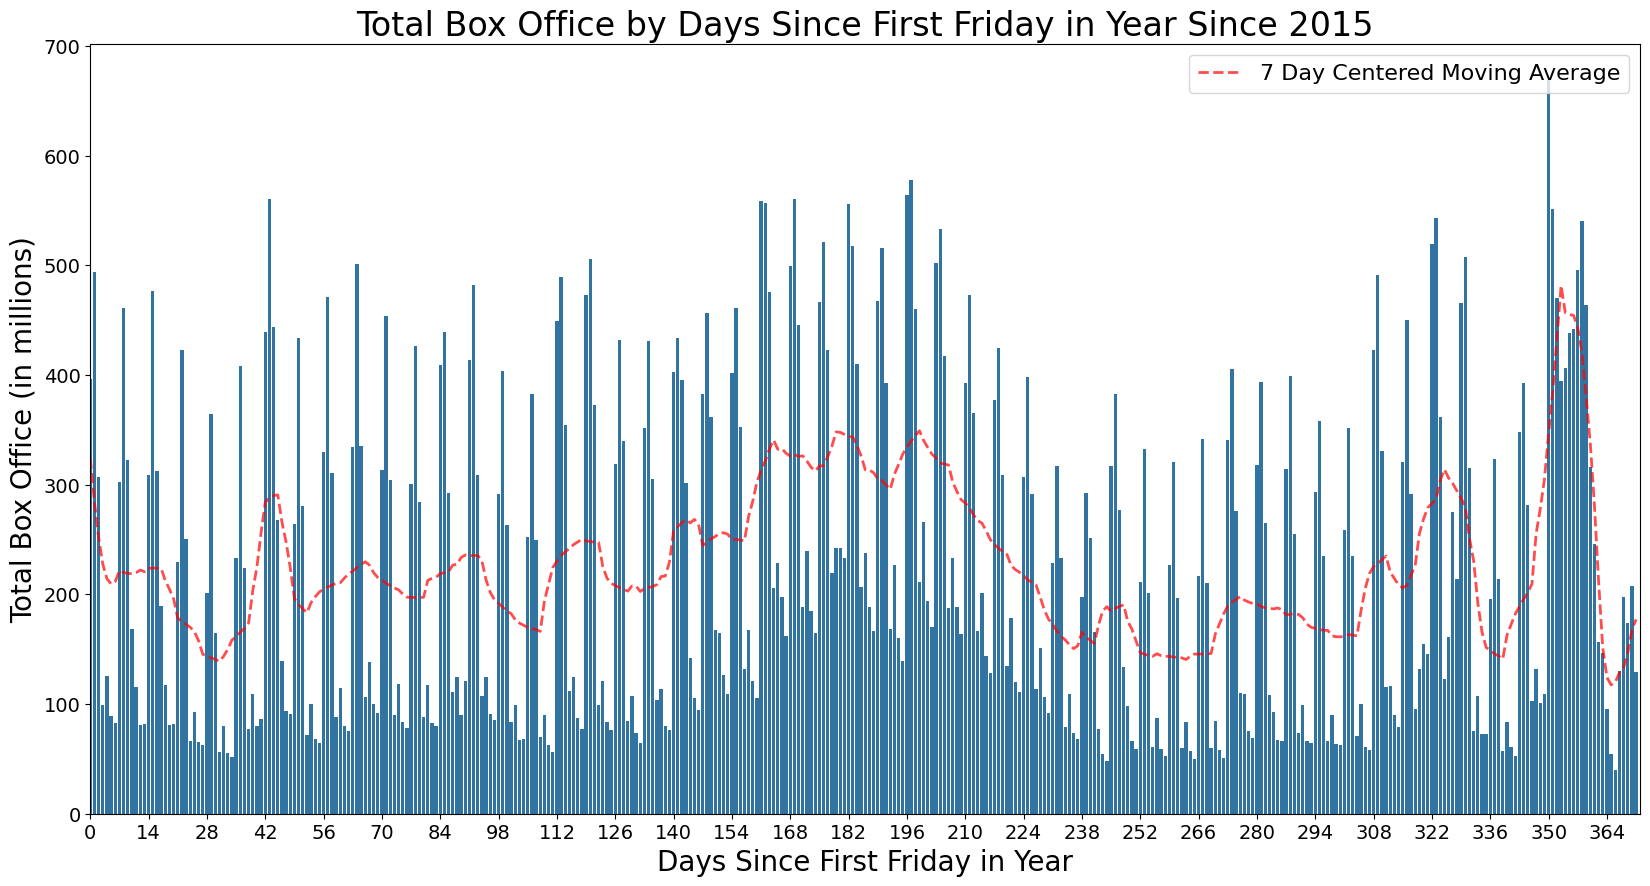
\includegraphics[width=1.0\textwidth]{../shared/images/boxoffice.png}
    \caption{This plot shows box office gross by days since the first Friday of the year. The x-axis is the number of days since the first Friday of the year which allows peaks to be aligned with the same day of the week. The y-axis is total gross since 2015. Nearly no matter the time of year, the box office is higher on weekends and holidays. During the time between Christmas and New Years, the box office is much higher than any other time of year. Additionally, weekdays are much higher in the summer than in the spring or fall.}
    \label{fig:seasonal}
\end{figure}

Within Figure \ref{fig:seasonal}, we can see that weekends have much higher grosses than weekdays with Saturdays higher than Fridays and Sundays. Additionally, some peaks are four days wide, corresponding to holidays that are on Mondays and always the same number of days after the first Friday (e.g. Memorial Day or MLK Day).

To account for seasonal performance differences, we created a seasonal multiplier value for each day of the year and holiday. The goal of this is to cancel out the impact of seasonality or holidays but not to cancel out the impact of day of week. 

To implement this multiplier, we need some baseline for the financial expectations of a movie that is coming out on a specific day. We use a weighted average of theater count and budget for each day, seen in Figure \ref{fig:weighteddays}.
\begin{figure}[H]
    \centering
    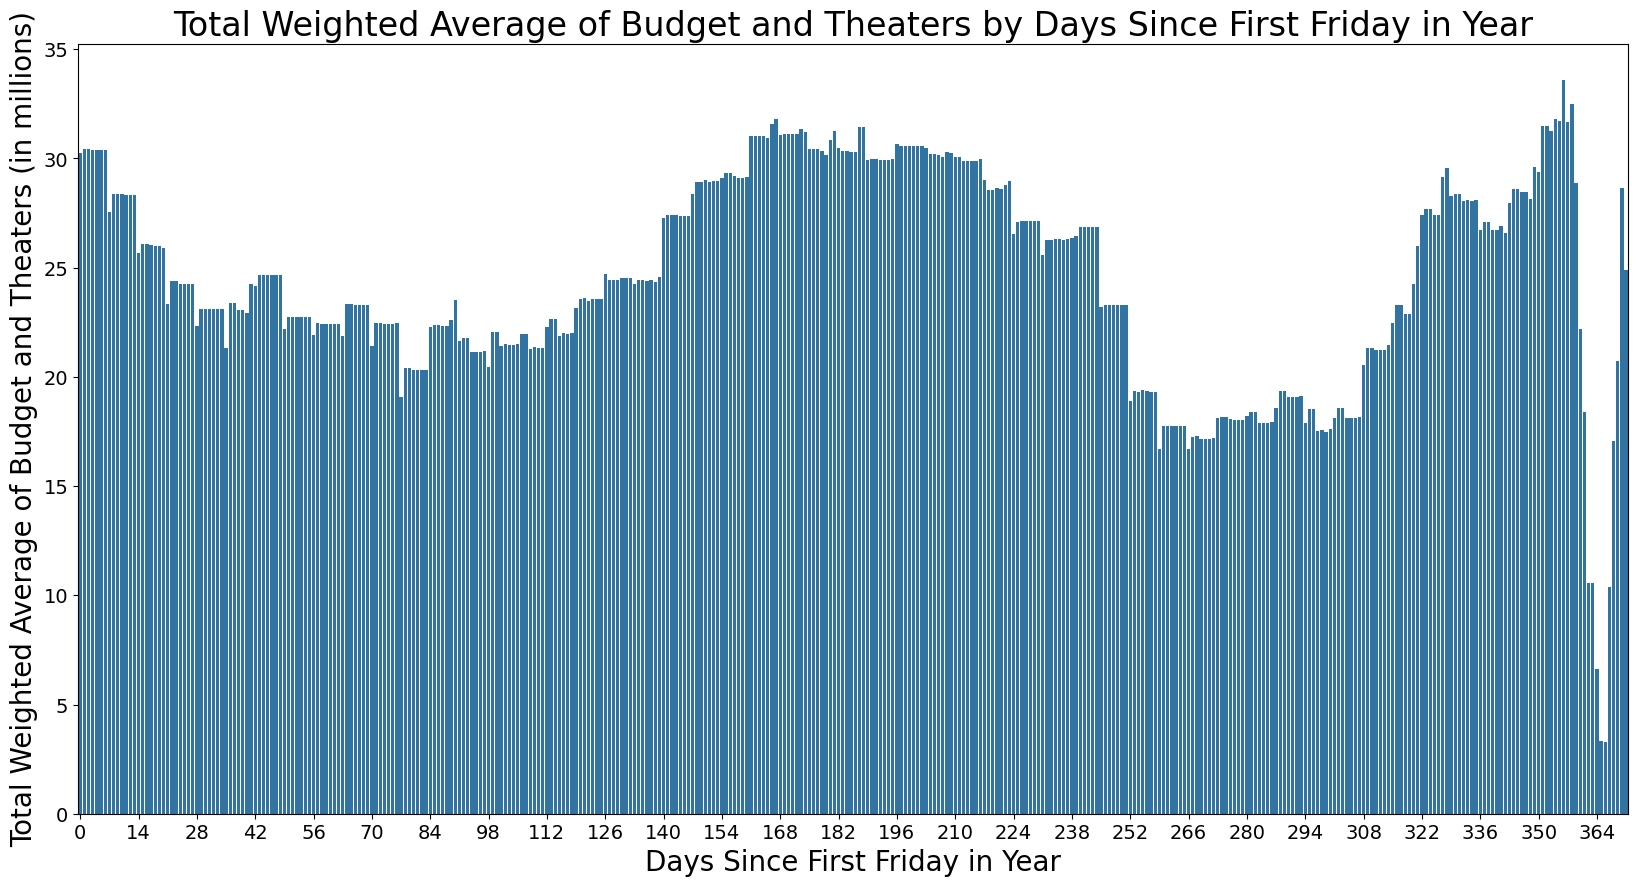
\includegraphics[width=1.0\textwidth]{../shared/images/weighteddays.png}
    \caption{This plot shows the weighted average of budget and theater count by days since first Friday of the year. The x-axis is the number of days since the first Friday of the year to match the previous figure. The y-axis is the weighted average of budget and theater count. The weighted average is calculated as the average of the budget and theater count for each day multiplied by the number of movies released on that day.}
    \label{fig:weighteddays}
\end{figure}

Based on this figure, it is clear that studios release more expensive movies during the summer and winter so we would expect those time periods to perform better. However, more expensive movies do not account for the entire difference in performance so adjustments are still needed. 

To create these multipliers, we tag every day with its day index since the first Friday of the year and any holidays. Holidays take priority over day of year. Then, we take the median gross for each day, balance it against the weighted average of budget and theaters, and multiply by the average gross for that day of week. 

\begin{equation}
    \text{seasonal\_multiplier} = \frac{\text{median gross for day}}{\text{average gross for day of week}} \times \frac{\text{average gross for day}}{\text{weighted average gross for day}}
\end{equation}

This normally gets a number around 1.0 and serves as the seasonal multiplier for that day. These multipliers are then weighted by recency based on the year they are from.
The lowest multiplier is 0.3766 for 244 days after the first Friday (falling around September 1st) and the highest multiplier is 3.1164 for 362 days after the first Friday (falling around December 31st). This multiplier decreases for the days around September because big-budget summer movies are still in theaters, but children are back in school, so movies gross less. Contrastingly, multipliers increase for the days around December due to holidays for adults and children alike.

All of the seasonal multipliers can be seen in Figure \ref{fig:seasonalmultipliers}.
\begin{figure}[H]
    \centering
    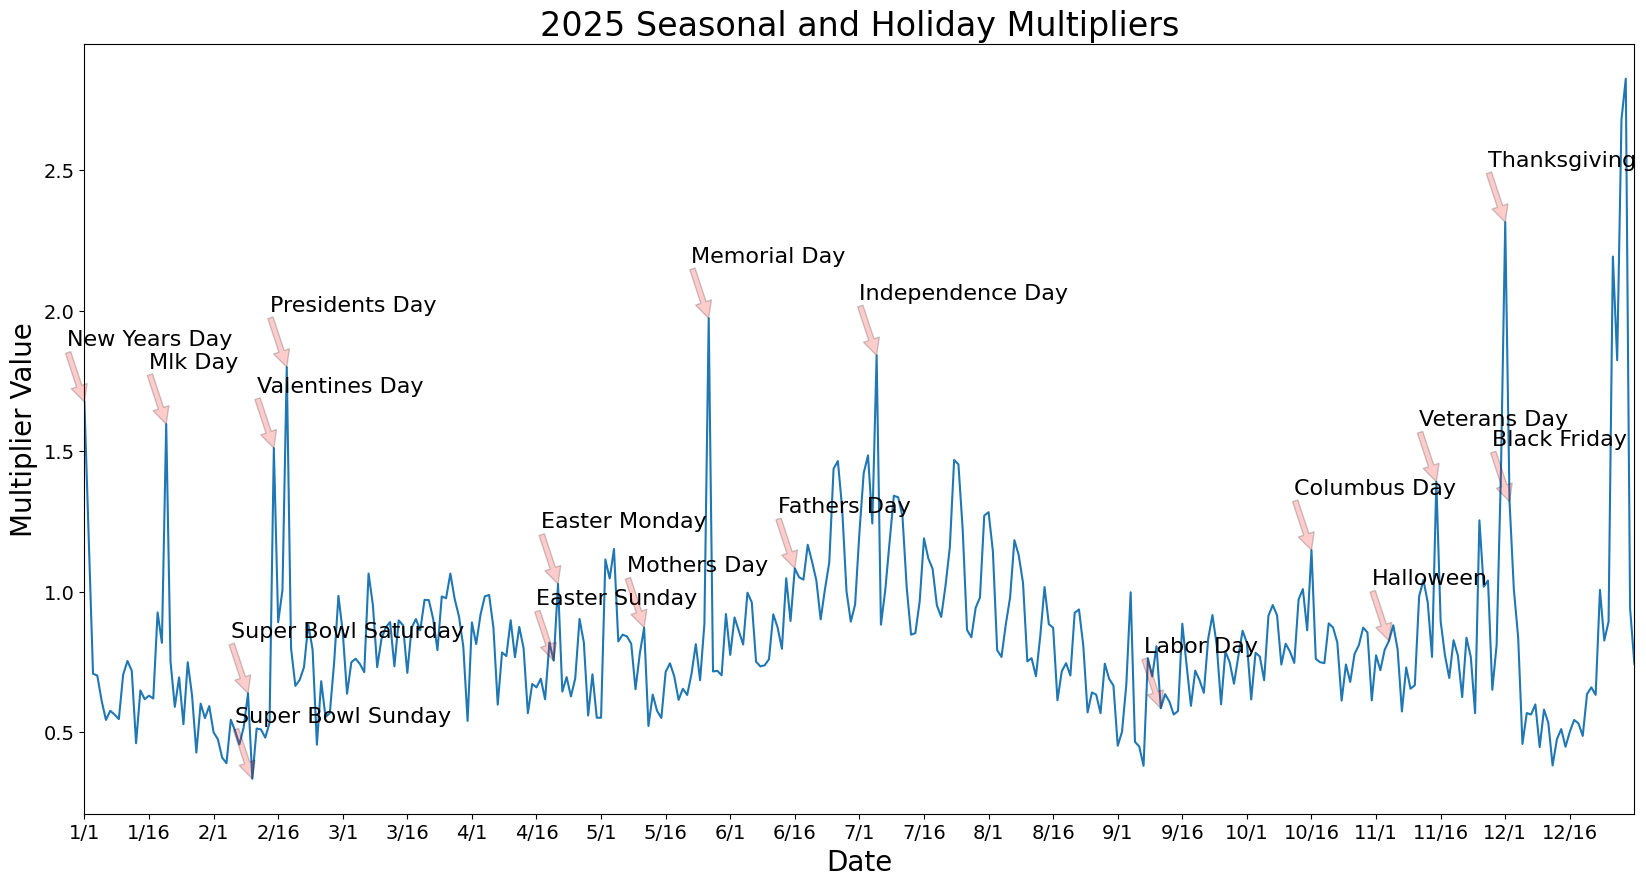
\includegraphics[width=1.0\textwidth]{../shared/images/adjustments.png}
    \caption{This plot shows the seasonal multipliers for each day of the year with annotations for holidays in 2025. The x-axis is the date in 2025 and the y-axis is multiplier value. Multipliers greater than 1 mean the box office performs better than average on that day. Some of the visible high multipliers include Valentine's Day, Thanksgiving Day, and the days between Christmas and New Years. The visible low multipliers include the days around Labor Day and Super Bowl Sunday.}
    \label{fig:seasonalmultipliers}
\end{figure}

\subsection{Comps}
One of the core ways to predict movie box office is to find comparable movies, or comps. Effective models must capitalize on the precedent set by similar movies. To find comps, we use a K-nearest neighbors (KNN) model with the following features (described in Section \ref{sssec:datafeatures}).
\begin{itemize}
    \item MPAA rating (G, PG, PG-13, R, etc.)
    \item Source (Original Screenplay, Based on Real Life Events, Based on Play, etc.)
    \item The Numbers genre (Comedy, Drama, Documentary, etc. (just one))
    \item Production method (Live Action, Animated, Hybrid, etc.)
    \item Creative type (Factual, Contemporary Fiction, Dramatization, etc.)
    \item Budget (squared percent difference)
    \item TMDB genres (Crime, Animation, Family, Music, Action, etc. (can have multiple))
    \item Spoken languages (English, Spanish, French, etc.)
    \item Production countries (United States, United Kingdom, France, etc.)
    \item Production companies (Warner Bros, Disney, etc.)
    \item Matching release types (Wide, Limited, etc.)
    \item Number of times released
\end{itemize}
Weights are found using randomized grid search. This process is demonstrated in Figures \ref{fig:gridsearch} and \ref{fig:gridsearchk} (appendix). This process found the optimal K value as \textbf{8} which will be used for the rest of the model. K is the number of comps to use for future model steps.

KNN uses the following distance metric:
Given weights $w_i$ where $i$ is each of the 12 features, the distance $d$ between two movies is given by:
\begin{equation}
d = \sum_{i=1}^{12} w_i \cdot (x_i - y_i)
\end{equation}
where $x_i$ and $y_i$ are the values of the features for the two movies. 
Then, the movies with the 8 lowest distances to the target movie are selected as the comps.

An example of the comps and multipliers can be seen in Figure \ref{fig:compsmultconclave} for \cite{conclave}.
Additional examples are in the appendix for \cite{barbie} \ref{fig:compsmultbarbie}, 
\cite{nosferatu} \ref{fig:compsmultnosferatu},
and \cite{redOne} \ref{fig:compsmultredone}.

\begin{figure}[H]
    \centering
    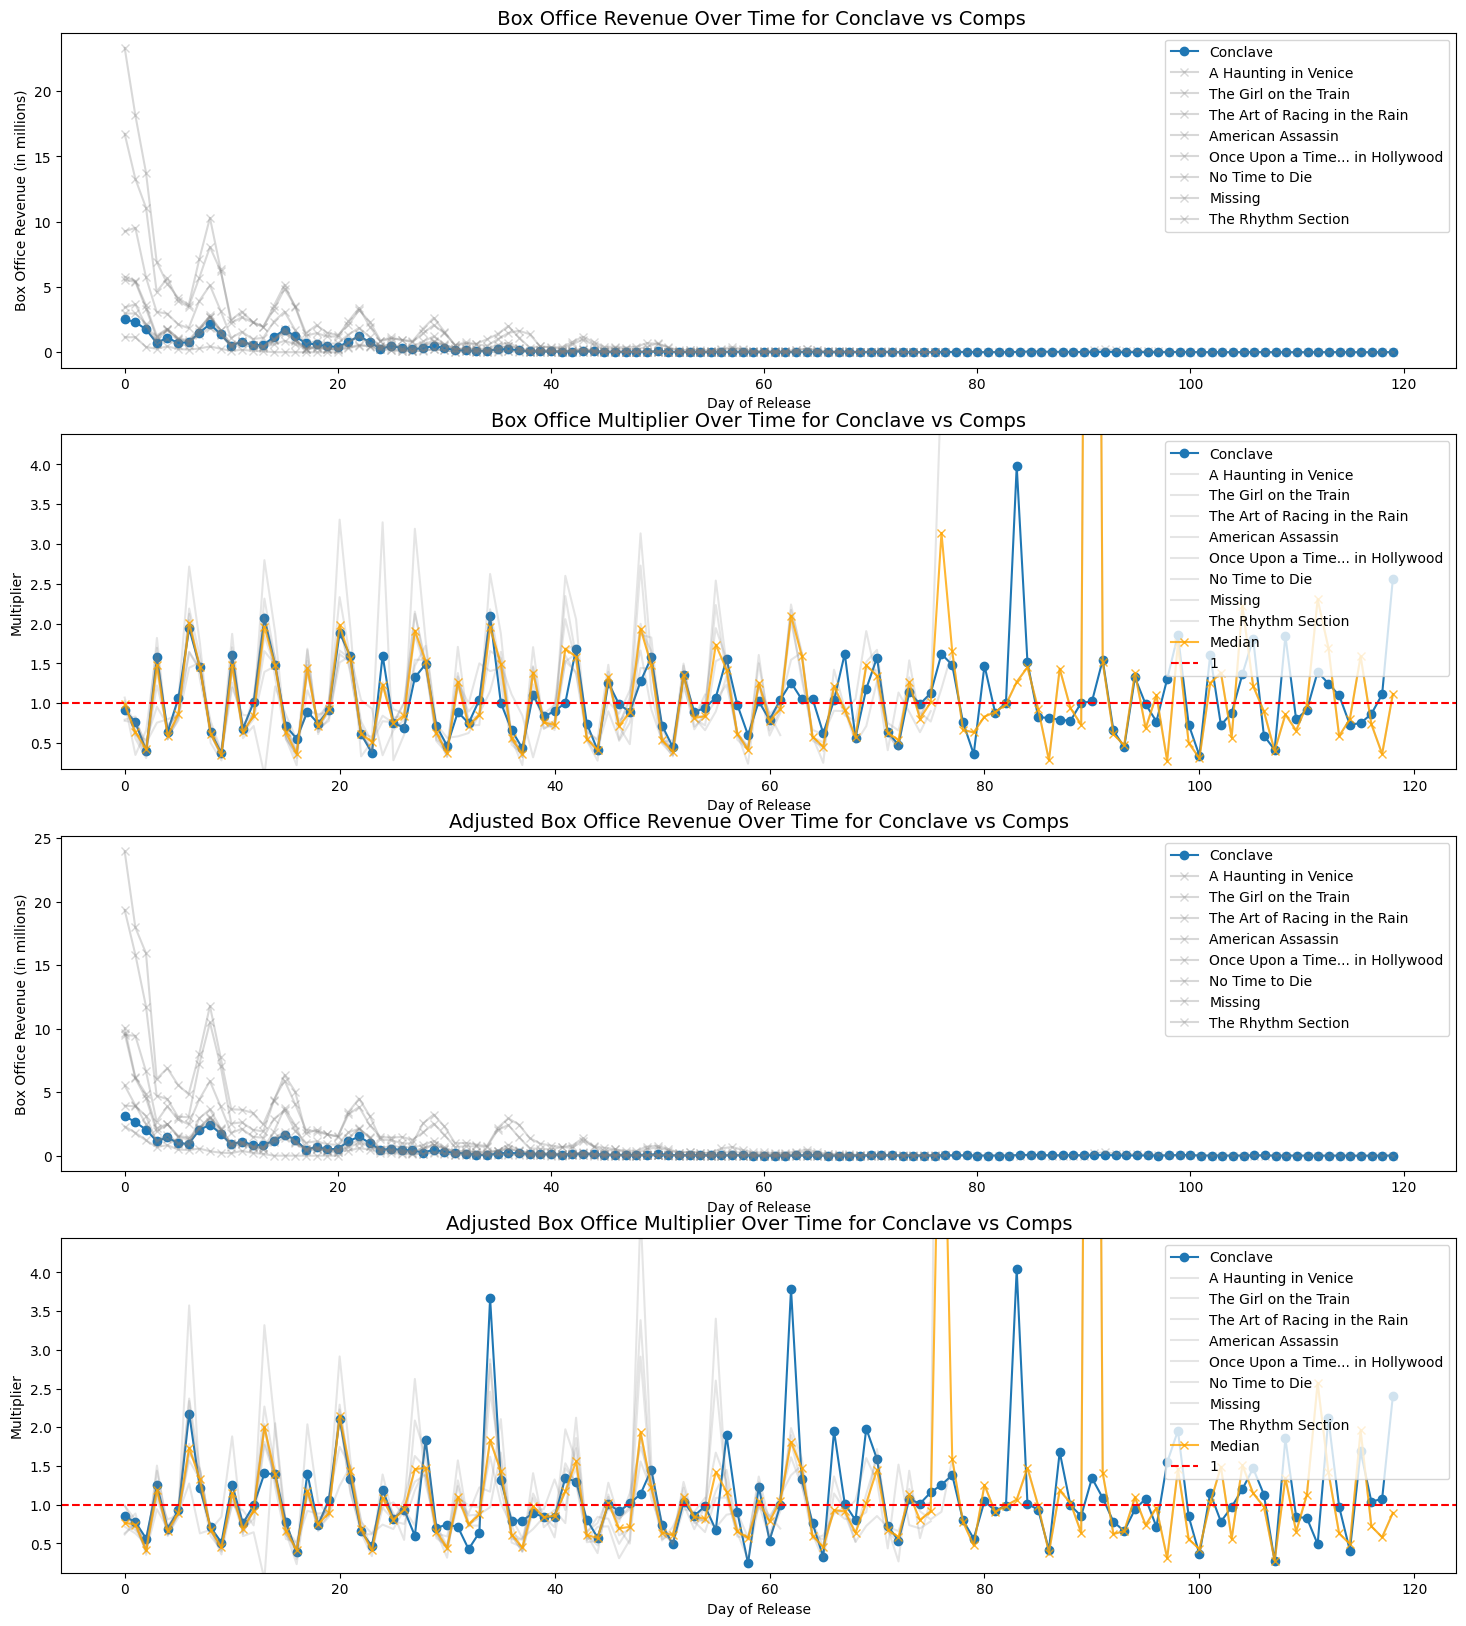
\includegraphics[width=0.9\textwidth]{../shared/images/compsmult/conclave.png}
    \caption{This plot shows comps and multipliers for \cite{conclave}. The top plot is box office revenue for Conclave and each of its comps; the second plot is multipliers for up to 120 days. The next two plots use adjusted gross instead of raw gross. Adjusted gross is based on of seasonal and holiday multipliers.}
    \label{fig:compsmultconclave}
\end{figure}

\subsection{Weekly Multipliers}

The next step is to figure out \textbf{weekly multipliers}. These can also be referred to as \textbf{weekly drops} since they are very frequently less than 1. Weekly multipliers are the percent change from one week to the next. As seen in Figure \ref{fig:weeklydrops}, movies generally drop in a geometric fashion that repeats similarly every week.

\begin{figure}[H]
    \centering
    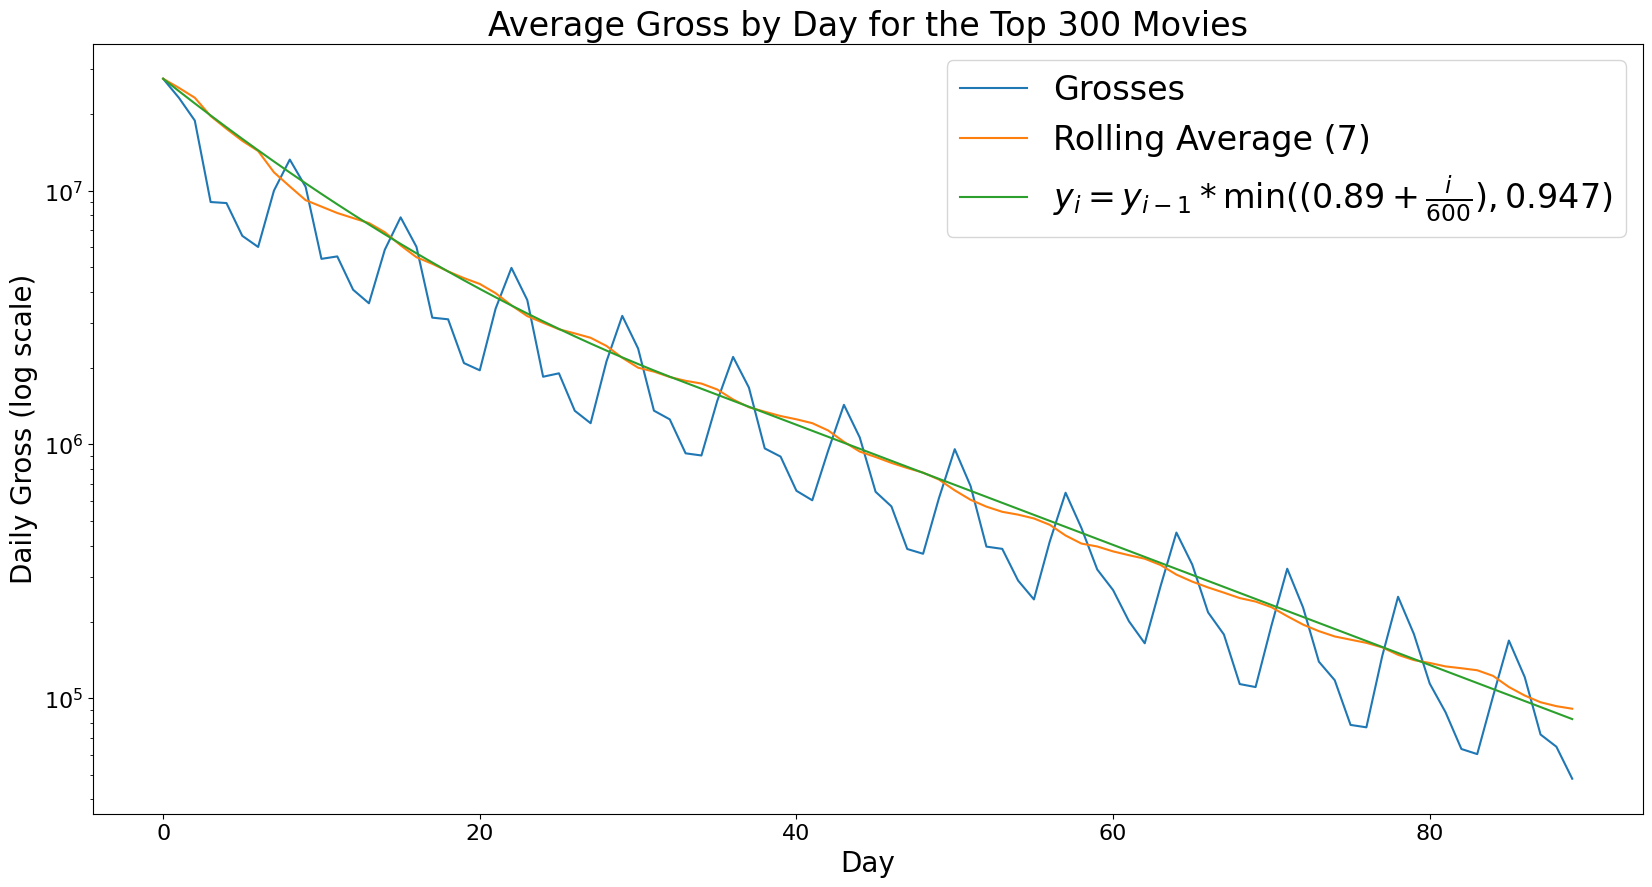
\includegraphics[width=0.7\textwidth]{../shared/images/top300fancy.png}
    \caption{This plot shows the average daily gross for the top 300 total grossing since 2015 over the first 90 days of their gross. There are peaks during weekends and troughs during weekdays. Additionally, a 7 day rolling average is included. Finally, there's a modified geometric series that almost exactly matches the rolling average demonstrating that a geometric series can be an effective model for weekly drops.}
    \label{fig:weeklydrops}
\end{figure}

To calculate weekly drops for a movie, we take the median weekly drop for each of the comps for that week. If the movie that we are currently predicting has been out for over 1 week, we also include its past history in predicting future weekly drops. This improves predictions because movies that drop a lot tend to continue to drop a lot, while movies that drop less tend to continue to drop less. This can be seen in Figure \ref{fig:otherdrops} (appendix).

\subsection{Daily Multipliers}

The final step of the modeling process is computing \textbf{daily multipliers}. Daily multipliers are the percent change from one day to the next. The average values for daily multipliers across all movies are shown in Table \ref{tab:drops}. These values are calculated based on the sum of overall box office gross on every day excluding movies in their first week of release. This is because movies in their first week of release have different multiplier patterns that are not representative of average multipliers. Box plots can be seen in Figure \ref{fig:multbyweekday} (appendix).

\begin{table}[H]
    \centering
    \begin{tabular}{lccccc}
        \toprule
        Day & Average Multiplier & Median Multiplier & Standard Deviation \\
        \midrule
        Monday → Tuesday & 1.21 & 1.28 & 0.32 \\
        Tuesday → Wednesday & 0.78 & 0.75 & 0.17 \\
        Wednesday → Thursday & 0.96 & 0.92 & 0.31 \\
        Thursday → Friday & 3.45 & 2.86 & 2.24 \\
        Friday → Saturday & 1.72 & 1.60 & 1.35 \\
        Saturday → Sunday & 0.69 & 0.66 & 0.16 \\
        Sunday → Monday & 0.40 & 0.35 & 0.20 \\
        \bottomrule
    \end{tabular}
    \caption{This table showcases the average, median, and standard deviation of daily multipliers. This highlights that the top grossing days are usually Friday and Saturday. Additionally, in general, the median multiplier is quite close to the average multiplier, which demonstrates that there are not huge tails either way. This pattern holds true for every day except for Friday which also has the largest standard deviation. This is because Fridays are when movies change theater counts and release types which can lead to large changes in box office gross.}
    \label{tab:drops}
\end{table}


When modeling the weekly drops, we take the median week-over-week drop for each of the comps. Then we apply that to the power of $\frac{1}{7}$ each day and multiply the daily multiplier for that day of the week.

Based on this, the overall equation for calculating the revenue on day n+1 is:

\begin{equation}
    \text{rev}_{n+1} = \text{rev}_{n} \times \text{weekly}_{\lfloor n/7 \rfloor}^{1/7} \times \text{daily}_{n \bmod 7} \times \frac{\text{seasonal}_{date_n+1}}{\text{seasonal}_{date_n}}
\end{equation}
where:
\begin{align*}
    \text{rev}_{n} &= \text{revenue on day n} \\
    \text{seasonal} &= \text{seasonal multiplier for the day of the year} \\
    \text{weekly} &= \text{array of the length that the movie is expected to be in theaters for} \\
    \text{daily} &= \text{array of the length 7 with daily multipliers for each day of the week} \\
\end{align*}

\subsection{Limited Releases} \label{sssec:limitedreleases}
This subproblem could be an entire project on its own. An example of a limited release movie is \cite{realPain} whose information can be seen below in Figure \ref{fig:compsmultrealpain}.

\begin{figure}[H]
    \centering
    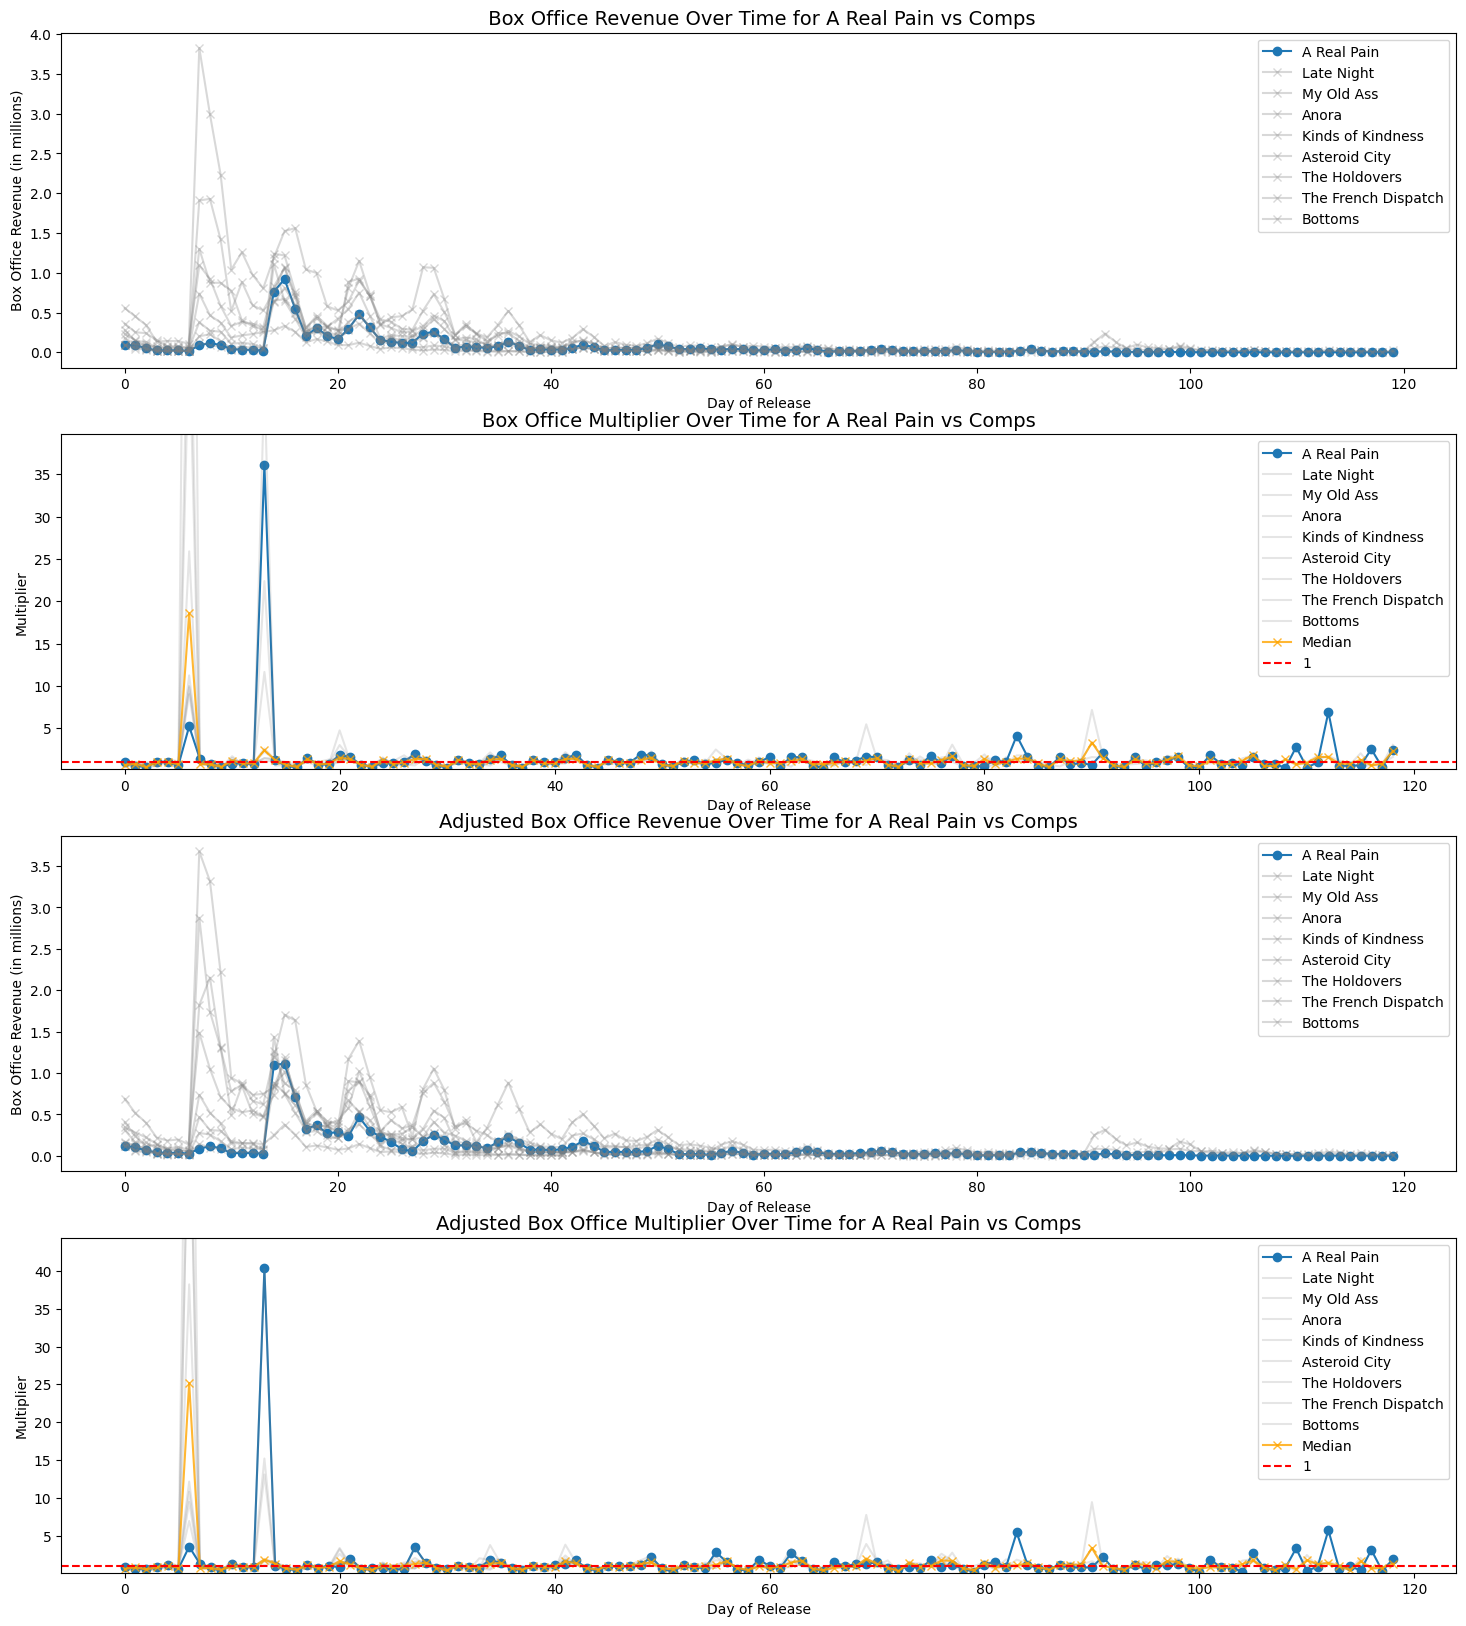
\includegraphics[width=1.0\textwidth]{../shared/images/compsmult/realpain.png}
    \caption{This plot shows comps and multipliers for \cite{realPain}. The top plot is box office revenue for A Real Pain and each of its comps; the second plot is multipliers for up to 120 days. The next two plots use adjusted gross instead of raw gross. Adjusted gross is based on seasonal and holiday multipliers.}
    \label{fig:compsmultrealpain}
\end{figure}

\textit{A Real Pain} started its release cycle in just 4 theaters before expanding to 12 and then finally to its peak of 1,185 theaters. A movie is considered in limited release if it is in under 1,000 theaters \citep{megalopolisMurrell}. The purpose of a limited release is to gain initial buzz and momentum or gauge audience interest. Lots of limited release movies come from independent studios, so they are riskier for theaters to show. Demonstrating positive buzz for the movie via a limited release can help convince theaters to show the movie wide \citep{limitedRelease}.

Figure \ref{fig:compsmultrealpain} illustrates that the various comps each go wide after different amounts of weeks: some after 1 week, some after 2 weeks (such as \textit{A Real Pain}), and some after 3 or even 4 weeks. Additionally, looking at the right side of the graphs, we can see that \textit{A Real Pain} had some very high multipliers around week 12; this coincided with Oscar nominations \citep{realPainNominated}. Since it was successful in the nominations, it expanded again after those were announced.

In order to deal with limited release movies expanding to wide release, we keep track of 2 sets of multipliers and weekly drops. The first set is for when the movie is in limited release and the second set is for when the movie is in wide release. Then, when the movie switches between release types, different multipliers are applied.

The only information given to the model regarding limited releases is date of release and release types. This leads to a problem with regards to theater counts. For example, \textit{A Real Pain} expanded from 12 to 1,185 theaters in one day. However another limited release movie, \cite{holdovers} was in 778 theaters before expanding to 1,478 for wide release. Unfortunately, the model cannot access information about expansion theater counts. This means that the accuracy for limited releases will generally be lower since the theater count patterns are much less consistent than for wide releases.

\subsection{Opening Day}

In the case where we predict movies before they come out, we need to predict the opening day gross. Then, after opening day is predicted, we can use the model as normal to predict the rest of the days.
To predict opening day, we train a robust multiple linear regression (RLM) algorithm on all previous movies and their opening day. We chose an RLM in this case because it is more robust to outliers and opening day is skewed. The RLM utilizes the Huber loss function which is a combination of squared loss at low values and absolute loss at high values. This is useful since opening day gross is very skewed and has a lot of outliers. We implement this model using the statsmodels library \citep{statsmodelsHome}.
After doing feature selection, our final model choice with coefficients is as follows:

\begin{dmath}
    opening\_day = 0.0719 \times budget + 0.5205 \times wiki\_views \times (1 - in\_franchise) + 7.7492 \times wiki\_views \times in\_franchise + 4.967e-08 \times wiki\_views \times yt\_views
\end{dmath}

where:
\begin{align*}
    \text{opening\_day} &= \text{opening day revenue} \\
    \text{budget} &= \text{budget of the movie} \\
    \text{wiki\_views} &= \text{cumulative wikipedia views of the movie in the first 30 days before movie release} \\
    \text{yt\_views} &= \text{youtube views of the movie trailer measured the day before movie release} \\
    \text{in\_franchise} &= \text{binary variable that is 1 if the movie is part of a franchise and 0 otherwise} \\
\end{align*}

Below is an actual vs predicted graph for the opening day revenue of the 100 most recent movies.

\begin{figure}[H]
    \centering
    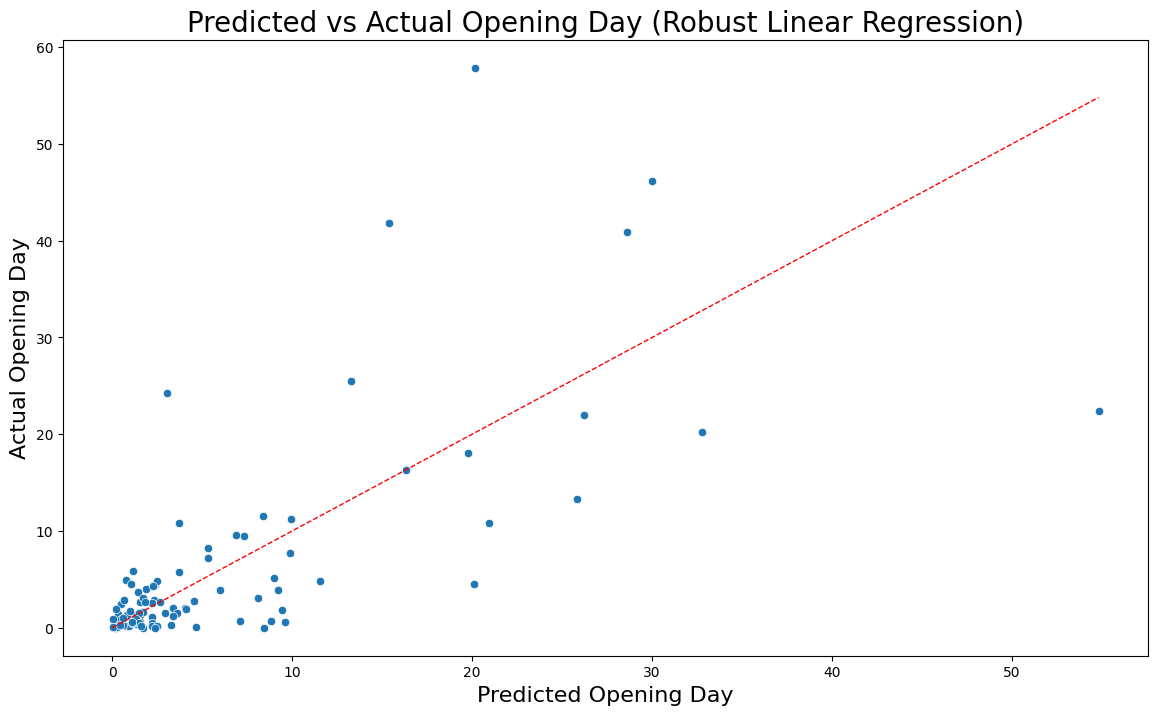
\includegraphics[width=0.9\textwidth]{../shared/images/predopeningday.png}
    \caption{This plot showcases performance of the robust multiple linear regression for predicting opening day gross on a test set of the 100 most recent movies. The $R^2$ value is 0.46 which is a reasonable starting point for the model. The x-axis is the predicted opening day gross and the y-axis is the actual opening day gross. The red line is the line of best fit. The model does a reasonable job of predicting opening day gross but there are some outliers.}
    \label{fig:openingday}
\end{figure}

Predicting opening day is a very challenging task since it is a higher variance than the rest of the movie gross. Overall, this component of the model does a reasonable job of predicting opening day and creates an acceptable starting point for the rest of the model. 

\subsection{Previews}
Previews are a special type of release where movies are released for a limited time before the official release date. Commonly, blockbuster movies will be available to watch after 3:00 PM on Thursday before the official Friday release \citep{previewTime}. However, in certain cases, movies will be released for up to a week before the official release date \citep{previews}. These previews are then wrapped into the opening day gross to augment the opening weekend. Out of the 500 most recent movies, roughly 30\% of them had previews as seen in Figure \ref{fig:previewpercent} (appendix).

\begin{figure}[H]
    \centering
    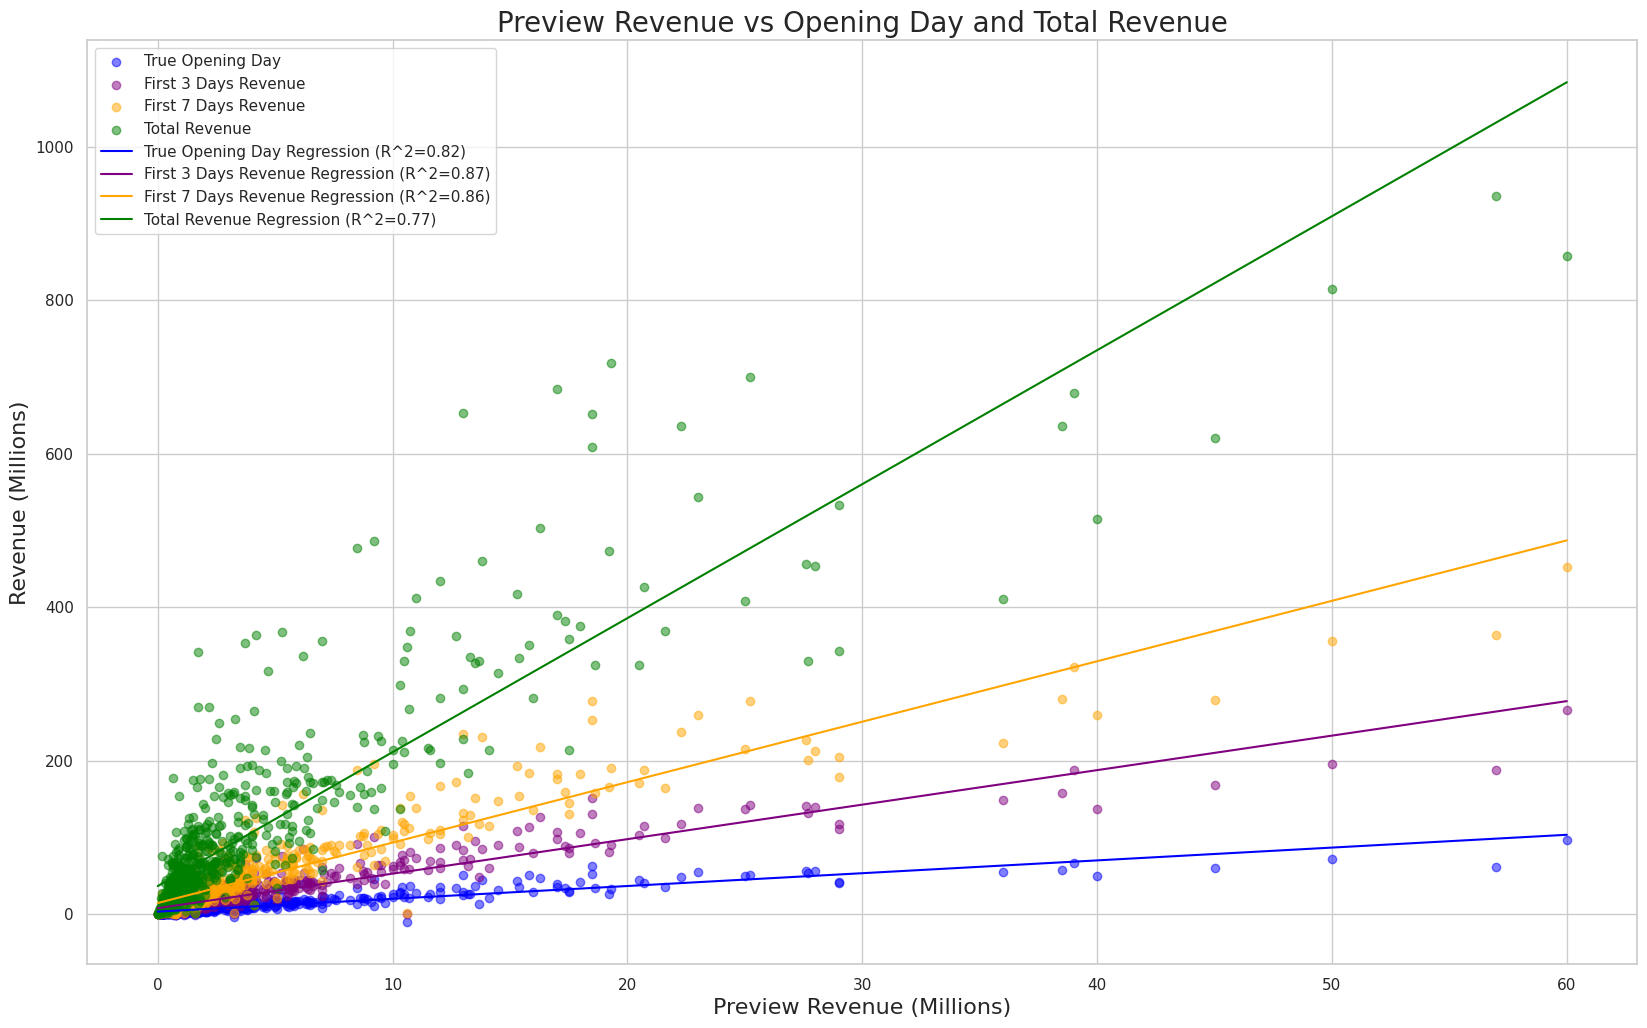
\includegraphics[width=1.0\textwidth]{../shared/images/previewopeningdays.png}
    \caption{This plot shows the correlation between preview grosses and true opening day, first 3 days, first 7 days, and total revenue. Additionally, there are linear regression lines for each series. The x-axis is the preview gross and the y-axis is the other gross. In general, the correlation between preview revenue and each of the revenue series is very high. The strongest is from previews to first 3 days with an $R^2$ of 0.87. The weakest is from previews to total revenue with an $R^2$ of 0.77.}
    \label{fig:previewopeningdays}
\end{figure}

To account for varying preview practices, the model utilizes true Fridays instead of preview-added Fridays. A true Friday is the studio-reported Friday gross with the previews removed.

\section{Results} \label{sec:results}

\begin{figure}[H]
    \centering
    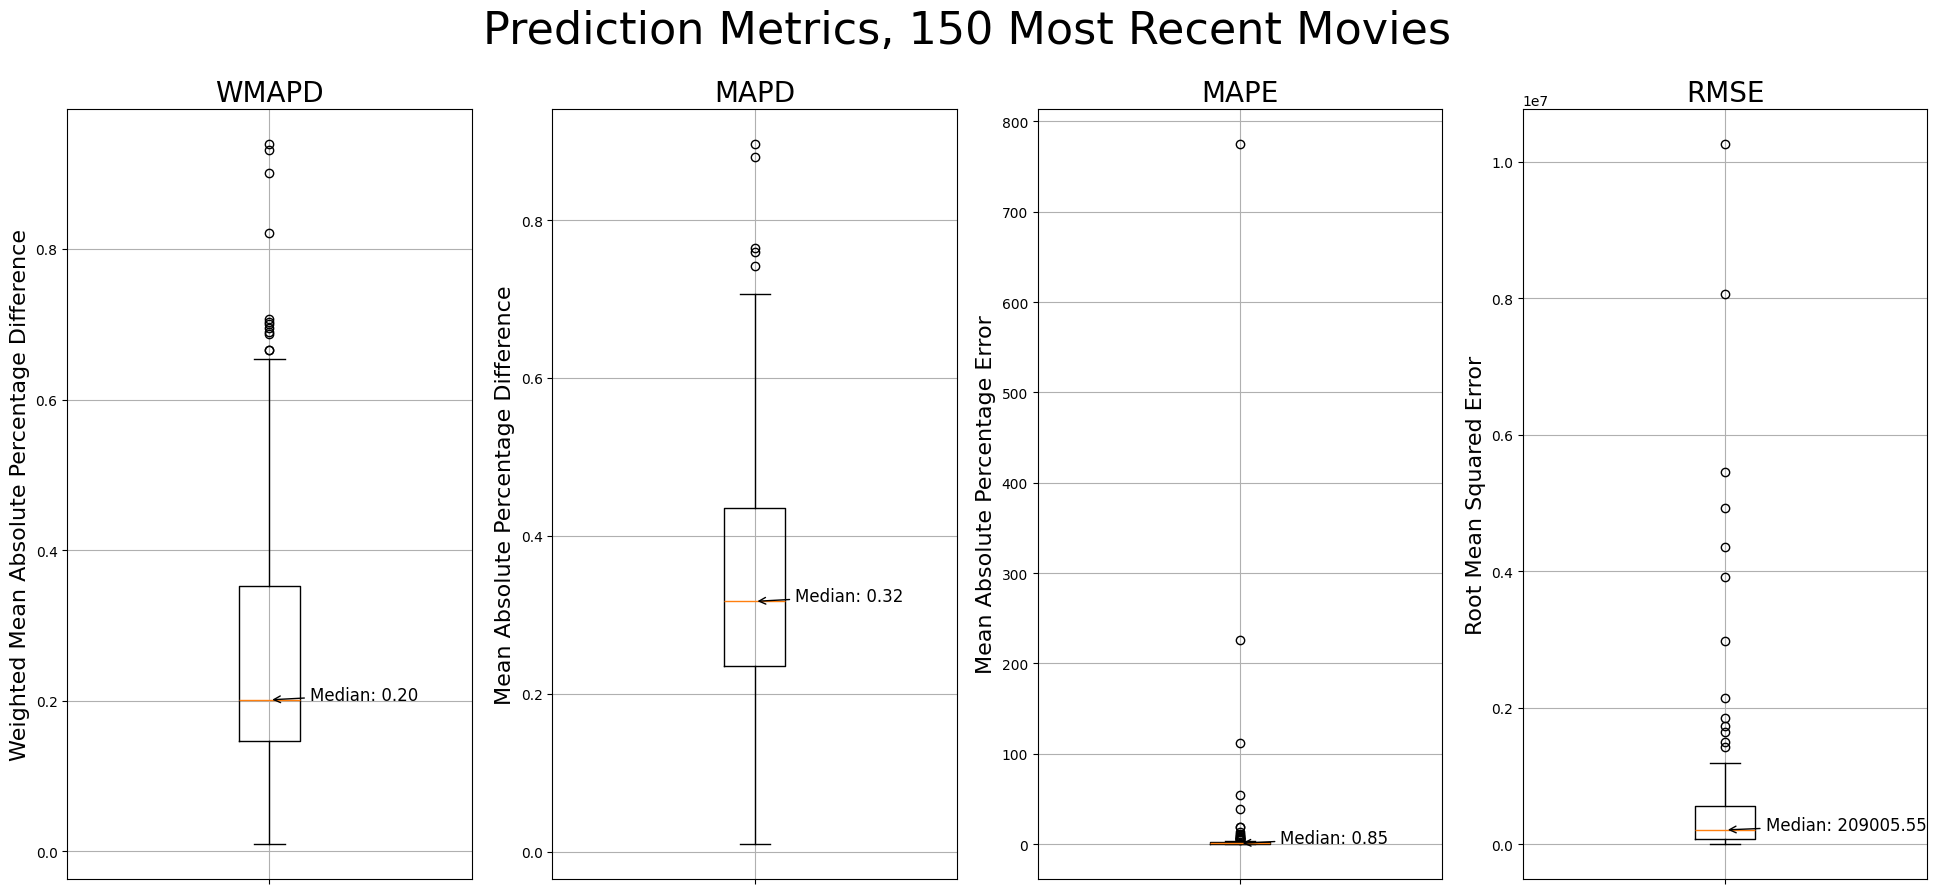
\includegraphics[width=1.0\textwidth]{../shared/images/results150.png}
    \caption{This plot showcases 4 box plots for each of the different relevant metrics. The median is annotated for each. The MAPE and RMSE have significant positive outlier tails whereas WMAPD and MAPD are more evenly distributed.}
    \label{fig:results}
\end{figure}

We present four different metrics for measuring model performance: WMAPD, MAPD, MAPE, and RMSE. In all cases, lower is better. Their formulas are as follows:

\textbf{Weighted Mean Absolute Percentage Difference (WMAPD):}
\begin{equation}
    \text{WMAPD} = \frac{\sum_{i=1}^{n} | y_i - \hat{y}_i |}{\sum_{i=1}^{n} \left( y_i + \hat{y}_i \right)}
\end{equation}

\textbf{Mean Absolute Percentage Difference (MAPD):}
\begin{equation}
    \text{MAPD} = \frac{\sum_{i=1}^{n} \frac{|y_i - \hat{y}_i|}{y_i+\hat{y}_i}}{n}
\end{equation}

\textbf{Mean Absolute Percentage Error (MAPE):}
\begin{equation}
    \text{MAPE} = \frac{\sum_{i=1}^{n} \frac{|y_i - \hat{y}_i|}{y_i}}{n}
\end{equation}

\textbf{Root Mean Squared Error (RMSE):}
\begin{equation}
    \text{RMSE} = \sqrt{\frac{\sum_{i=1}^{n} (y_i - \hat{y}_i)^2}{n}}
\end{equation}

Although the other metrics are more common, WMAPD is the most useful metric in our case. Unlike other metrics, it accounts for the problem of compounding errors more effectively. These metrics are calculated from predictions made using only the opening day's box office gross and categorical movie details. If just the first multiplier is wrong, all future predictions will be affected by that incorrect result. WMAPD assigns higher weights to larger box office days. Since the higher-grossing are normally earlier in the gross, this means that the model will be penalized more for being wrong on the first few days. This is a good thing since the model should be able to predict the first few days better than later days. 
One other consideration was implementing the weights simply as the number of days predicted minus the current prediction index. We decided not to implement WMAPD in this manner because overall larger days are more impactful, and so for cases such as limited release movies, the model should still focus more on larger grosses rather than earlier days.

Below are some results for specific movies to help contextualize WMAPD. First, Figure \ref{fig:predtwisters} shows the results for \cite{twisters}.

\begin{figure}[H]
    \centering
    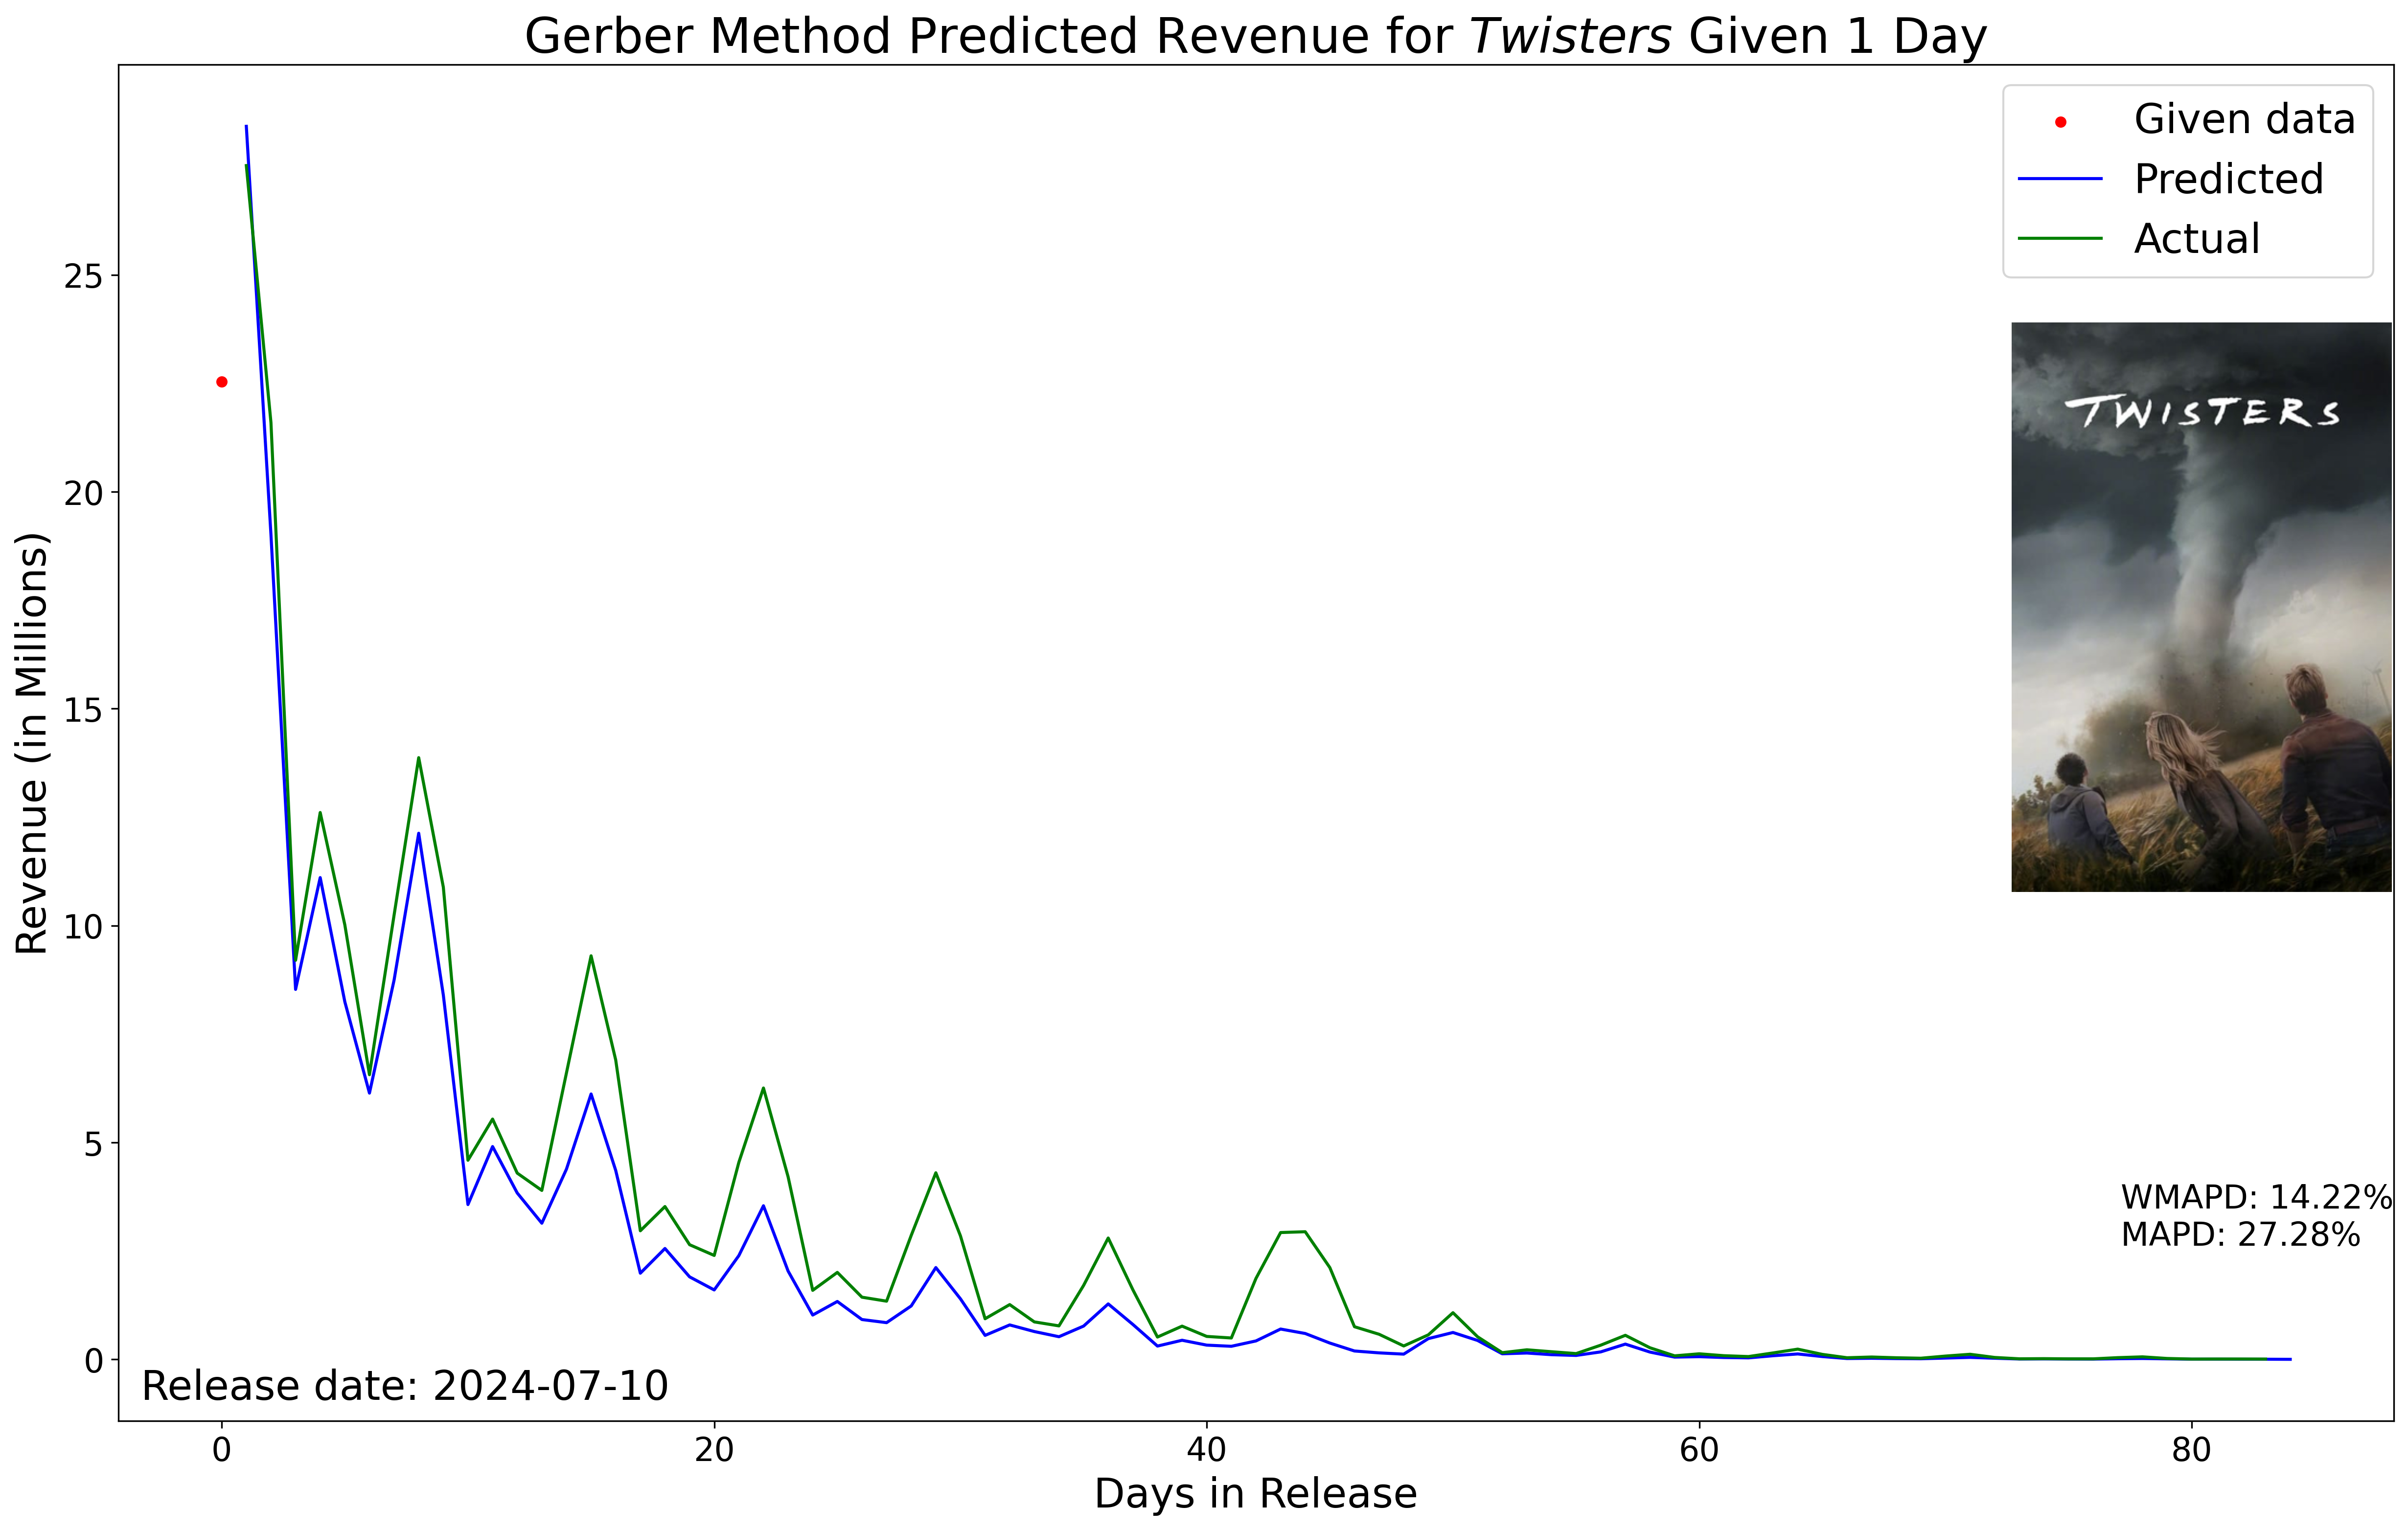
\includegraphics[width=0.769\textwidth]{../shared/images/pred/Twisters_1.png}
    \caption{This plot presents predictions for \cite{twisters} given 1 day.}
    \label{fig:predtwisters}
\end{figure}

This is an example of a slightly better than average result for overall performance. Some of the days, especially near the beginning, are very accurate. Additionally, the model does correctly respond to the day of the week. \textit{Twisters} is considered a movie that overperformed its box office expectations \citep{twistersBoxOffice,twistersMurrell}. These predictions show that Twisters achieved this by having smaller weekly drops than similar movies.

Next, lets take a look at a particularly bad prediction for \cite{jokerFolie} in Figure \ref{fig:predjoker}.

\begin{figure}[H]
    \centering
    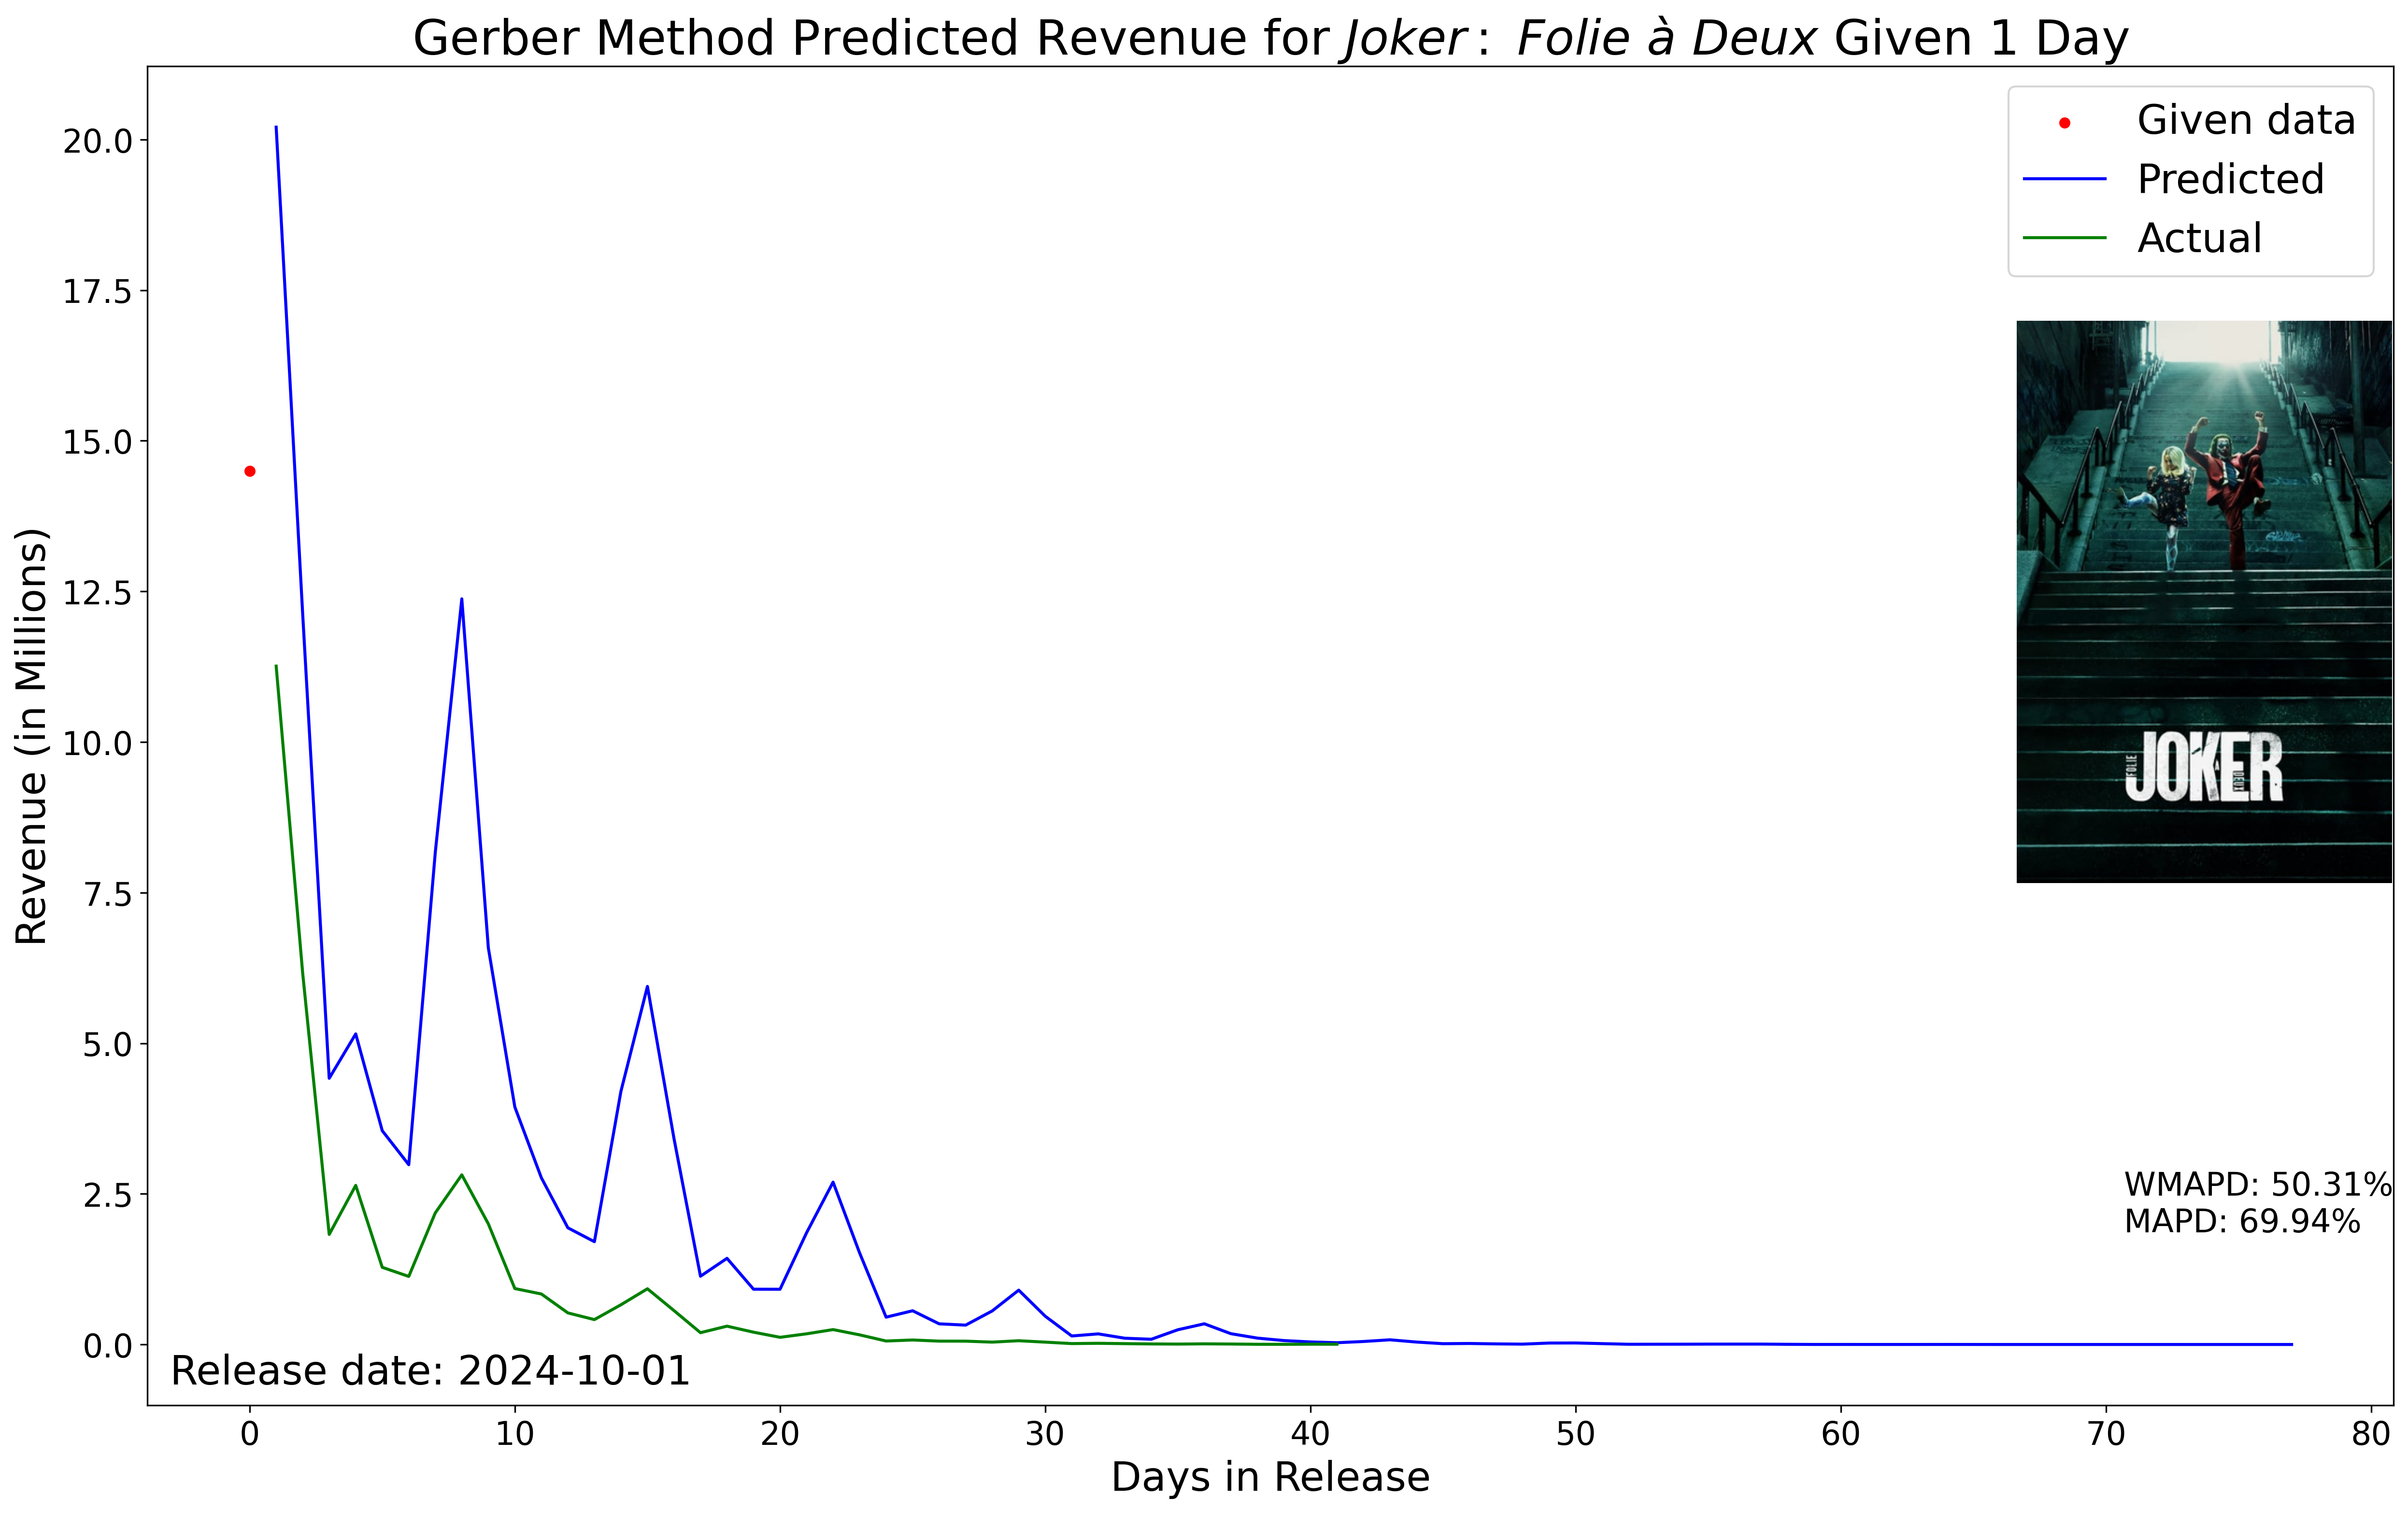
\includegraphics[width=0.769\textwidth]{../shared/images/pred/Joker: Folie à Deux_1.png}
    \caption{This plot presents predictions for \cite{jokerFolie} given 1 day.}
    \label{fig:predjoker}
\end{figure}

\textit{Joker 2} is one of the largest box office disappointments of all time \citep{joker2Murrell, joker2Cinemascore, polymarketHighestGrossing2024}. Due to this, the model over-predicts the gross. Cases such as \textit{Joker 2} are outside the bounds of the comps because there has simply never been a movie like \textit{Joker 2} that has performed this badly before. Notably, the daily patterns closely resemble the prediction but the weekly drops are much steeper than predicted.

Figure \ref{fig:predjokermulti} below shows predictions for Joker 2 when the model is provided with data from a varying number of days.

\begin{figure}[H]
    \centering
    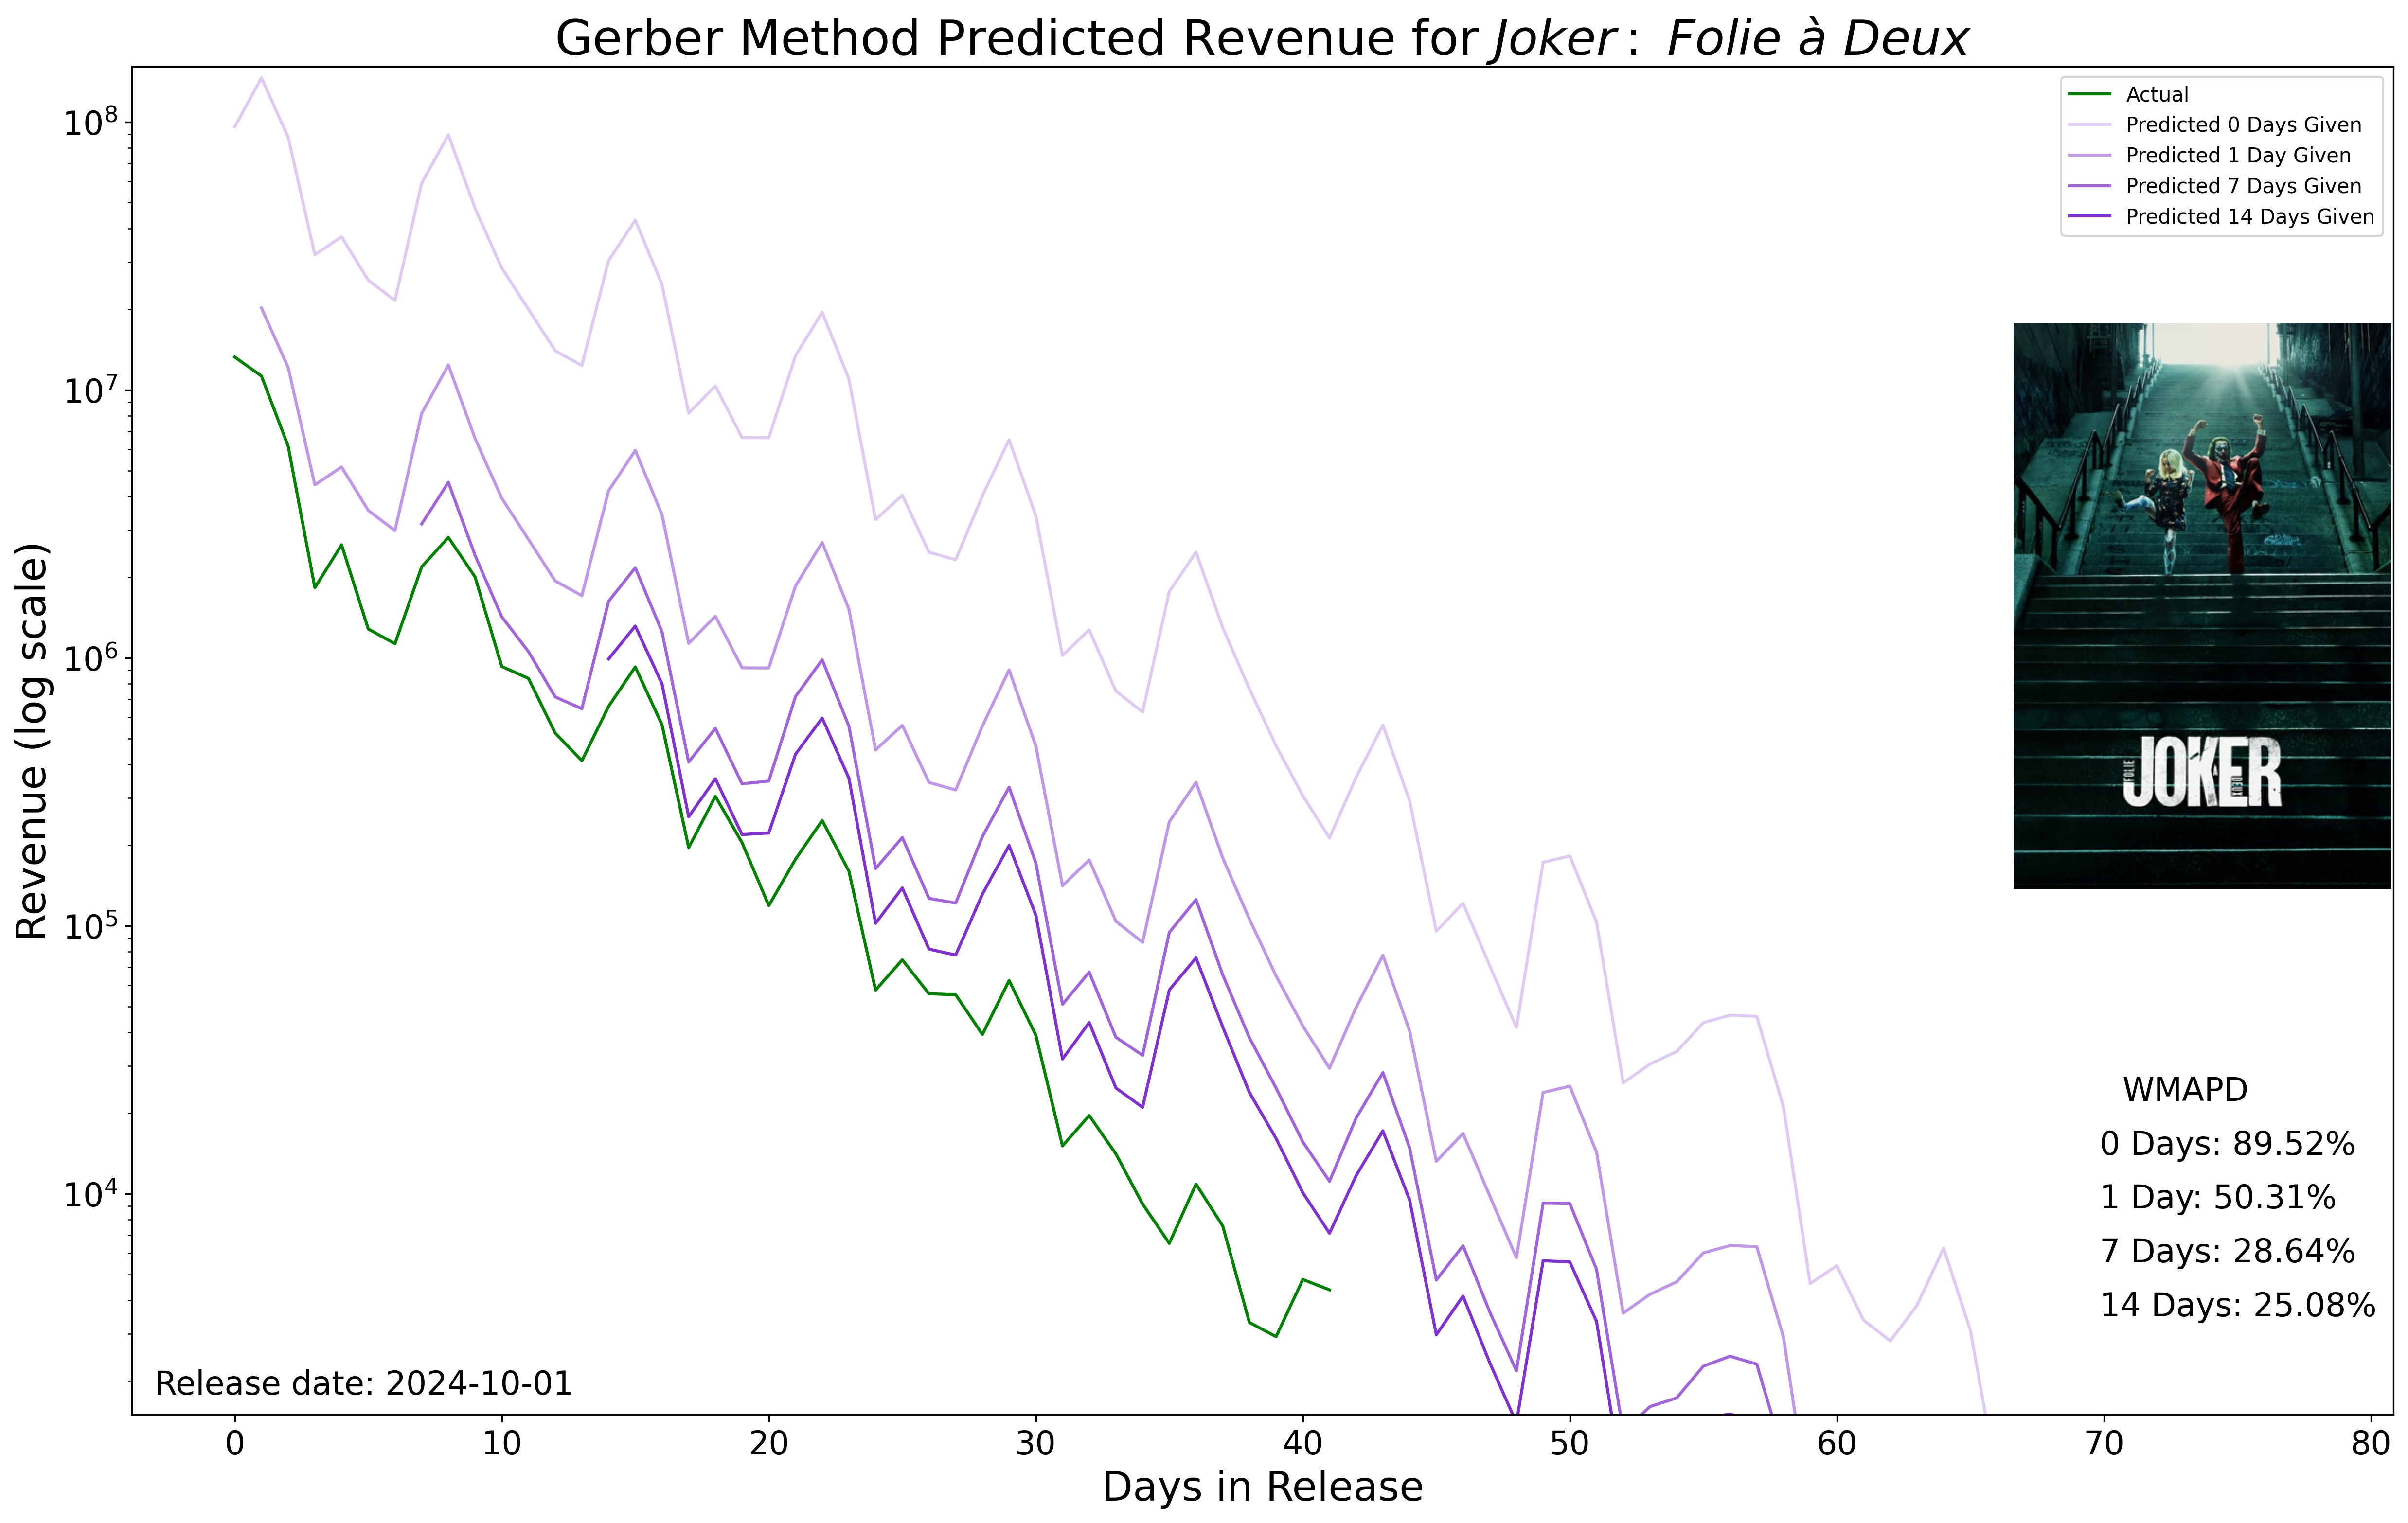
\includegraphics[width=0.769\textwidth]{../shared/images/pred/Joker: Folie à Deux_multiple_4.png}
    \caption{This plot presents predictions for \cite{jokerFolie} given 0, 1, 7, and 14 days.}
    \label{fig:predjokermulti}
\end{figure}

Within this plot, we can see that the model is able to improve its predictions over time. This is because as the model is given more days, it can adjust to Joker 2's underperformance and update future predictions accordingly.

Next, we examine a limited release example case for \cite{conclave} in Figure \ref{fig:predconclave}.

\begin{figure}[H]
    \centering
    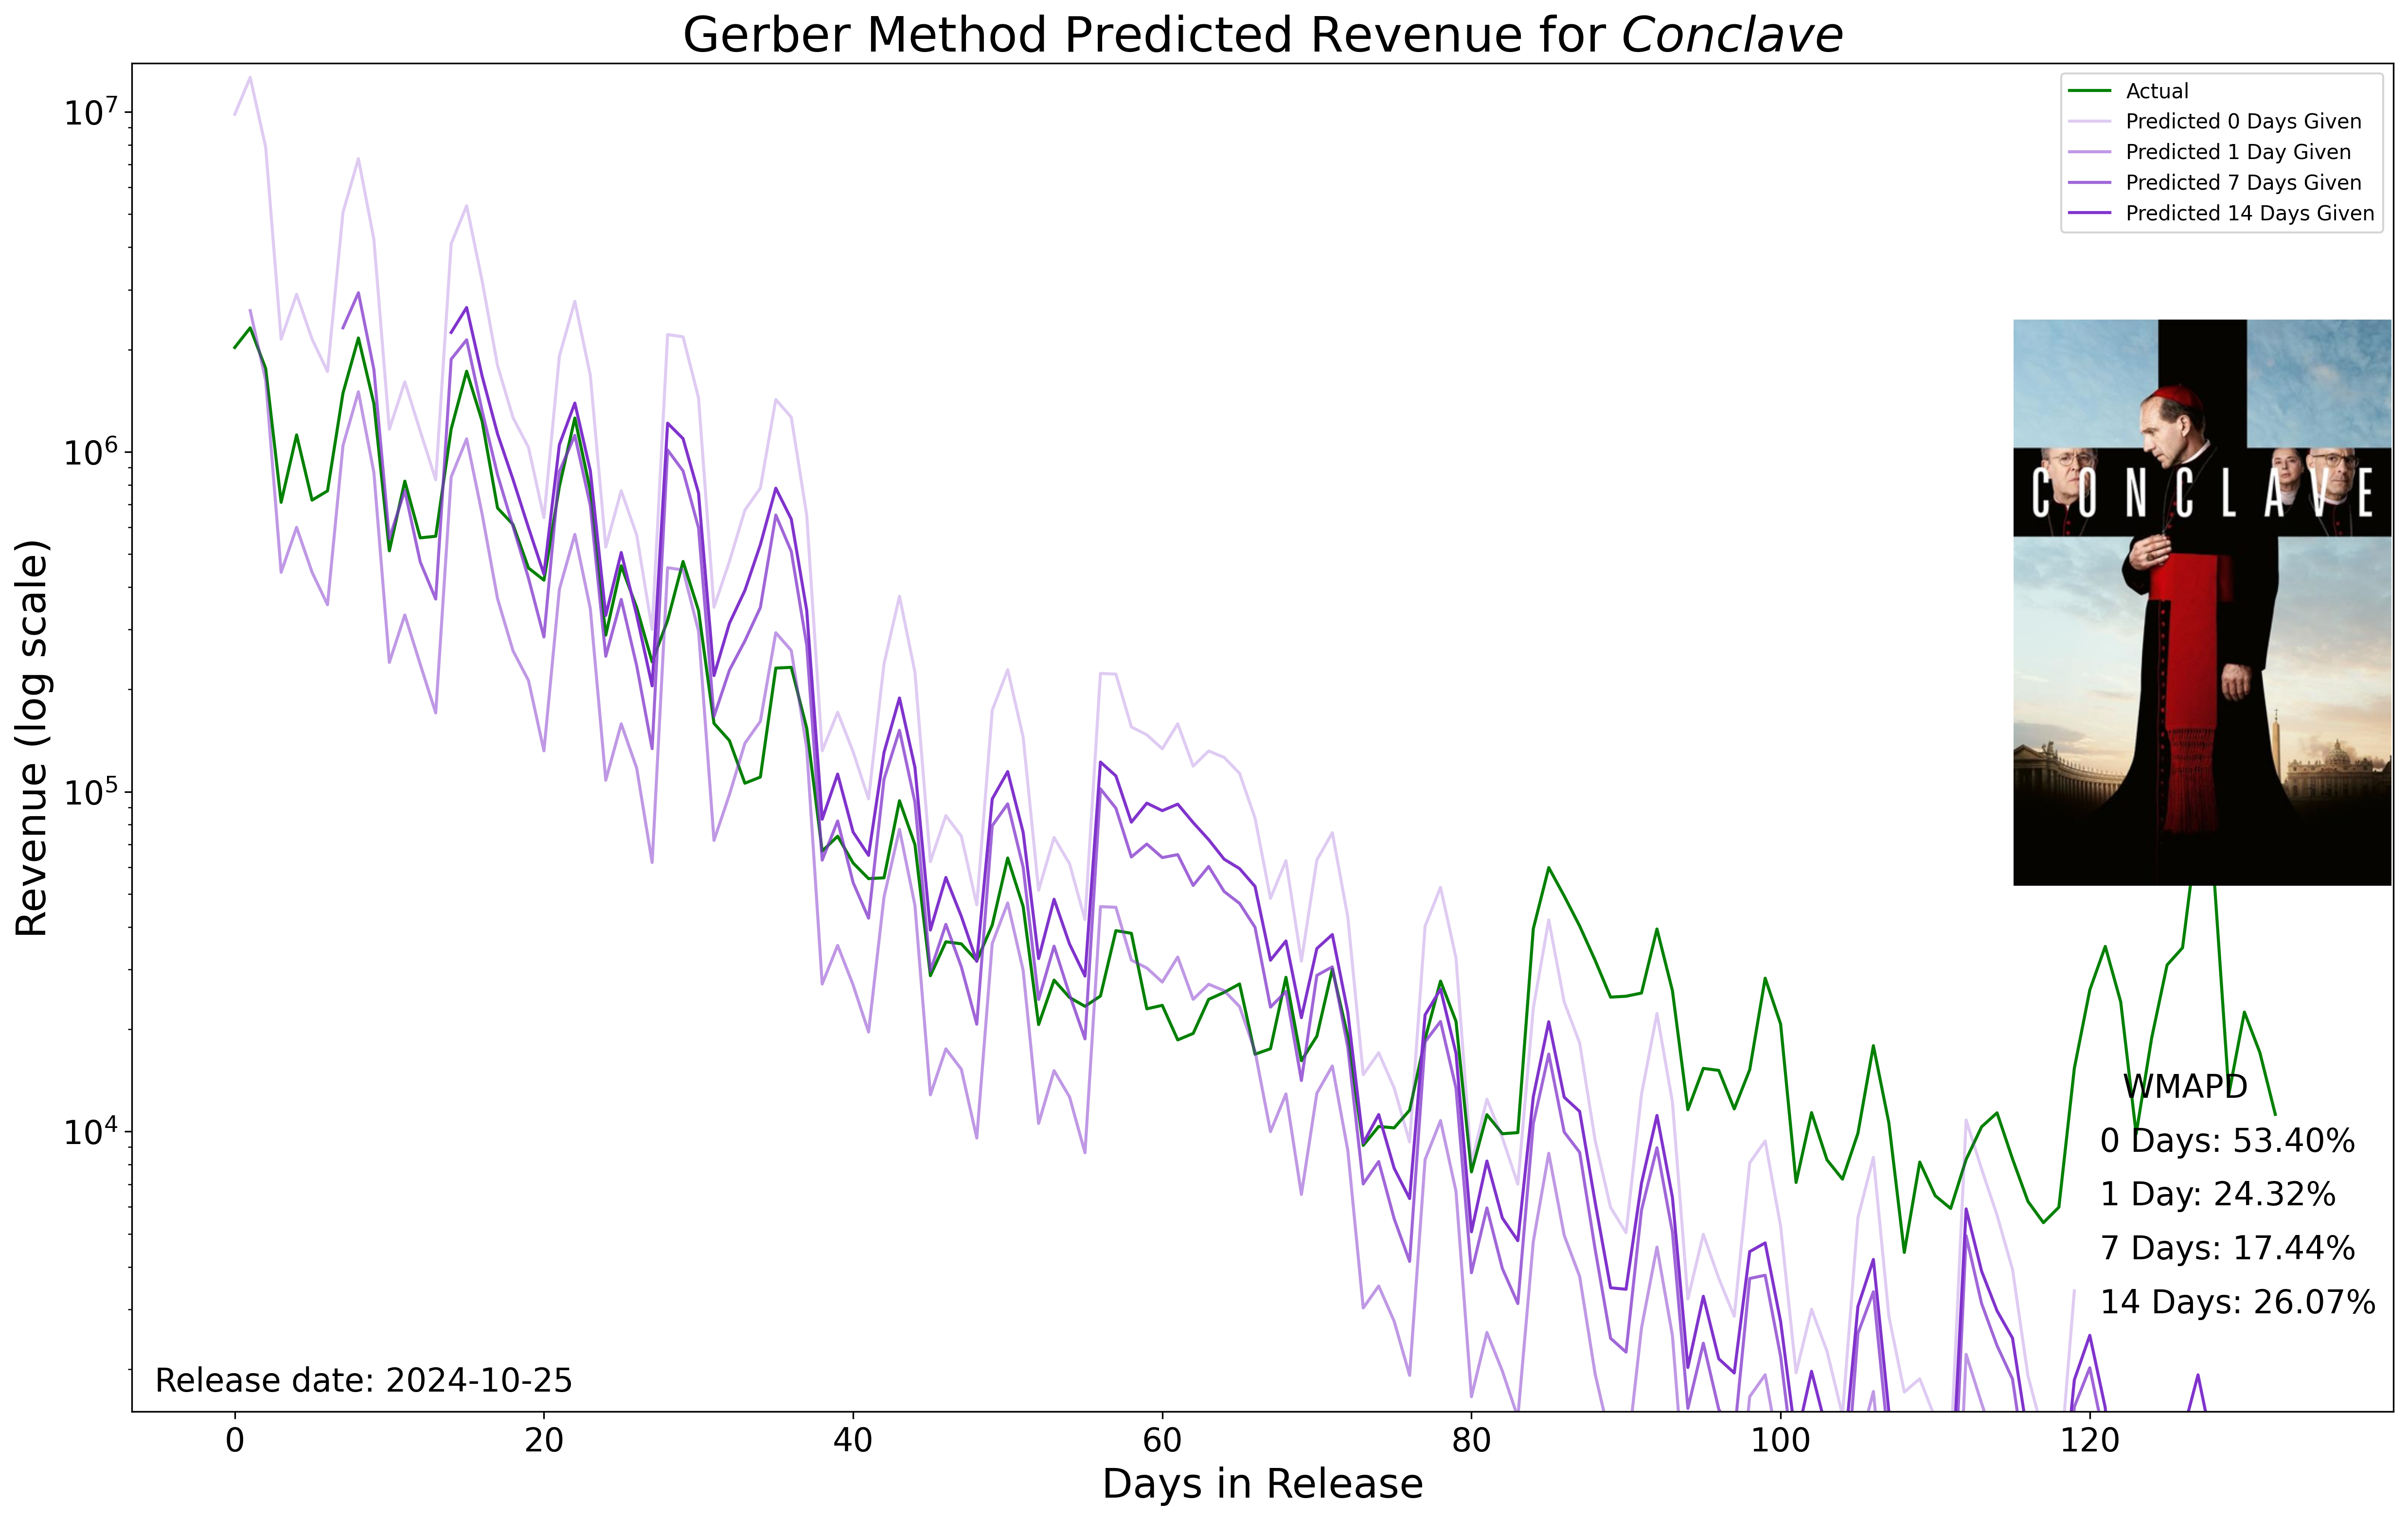
\includegraphics[width=0.769\textwidth]{../shared/images/pred/Conclave_multiple_4.png}
    \caption{This plot presents predictions for \cite{conclave} given 0, 1, 7, and 14 days.}
    \label{fig:predconclave}
\end{figure}

\textit{Conclave} was a midsize release which makes it considerably more challenging to predict. The model performs well initially. However, as \textit{Conclave} maintains theater count consistency even after 60 days of release, the predictions become somewhat scattered. Notably, the model expects \textit{Conclave} to remain in theaters for 120 days, though not at the high gross levels it actually achieved. This is because \textit{Conclave} generally received better reviews than its comps and consequently expanded theater count for Oscar nominations \citep{conclaveOscarNominations}.

One more strong example is \cite{insideOut2} in Figure \ref{fig:predinsideout}.
\begin{figure}[H]
    \centering
    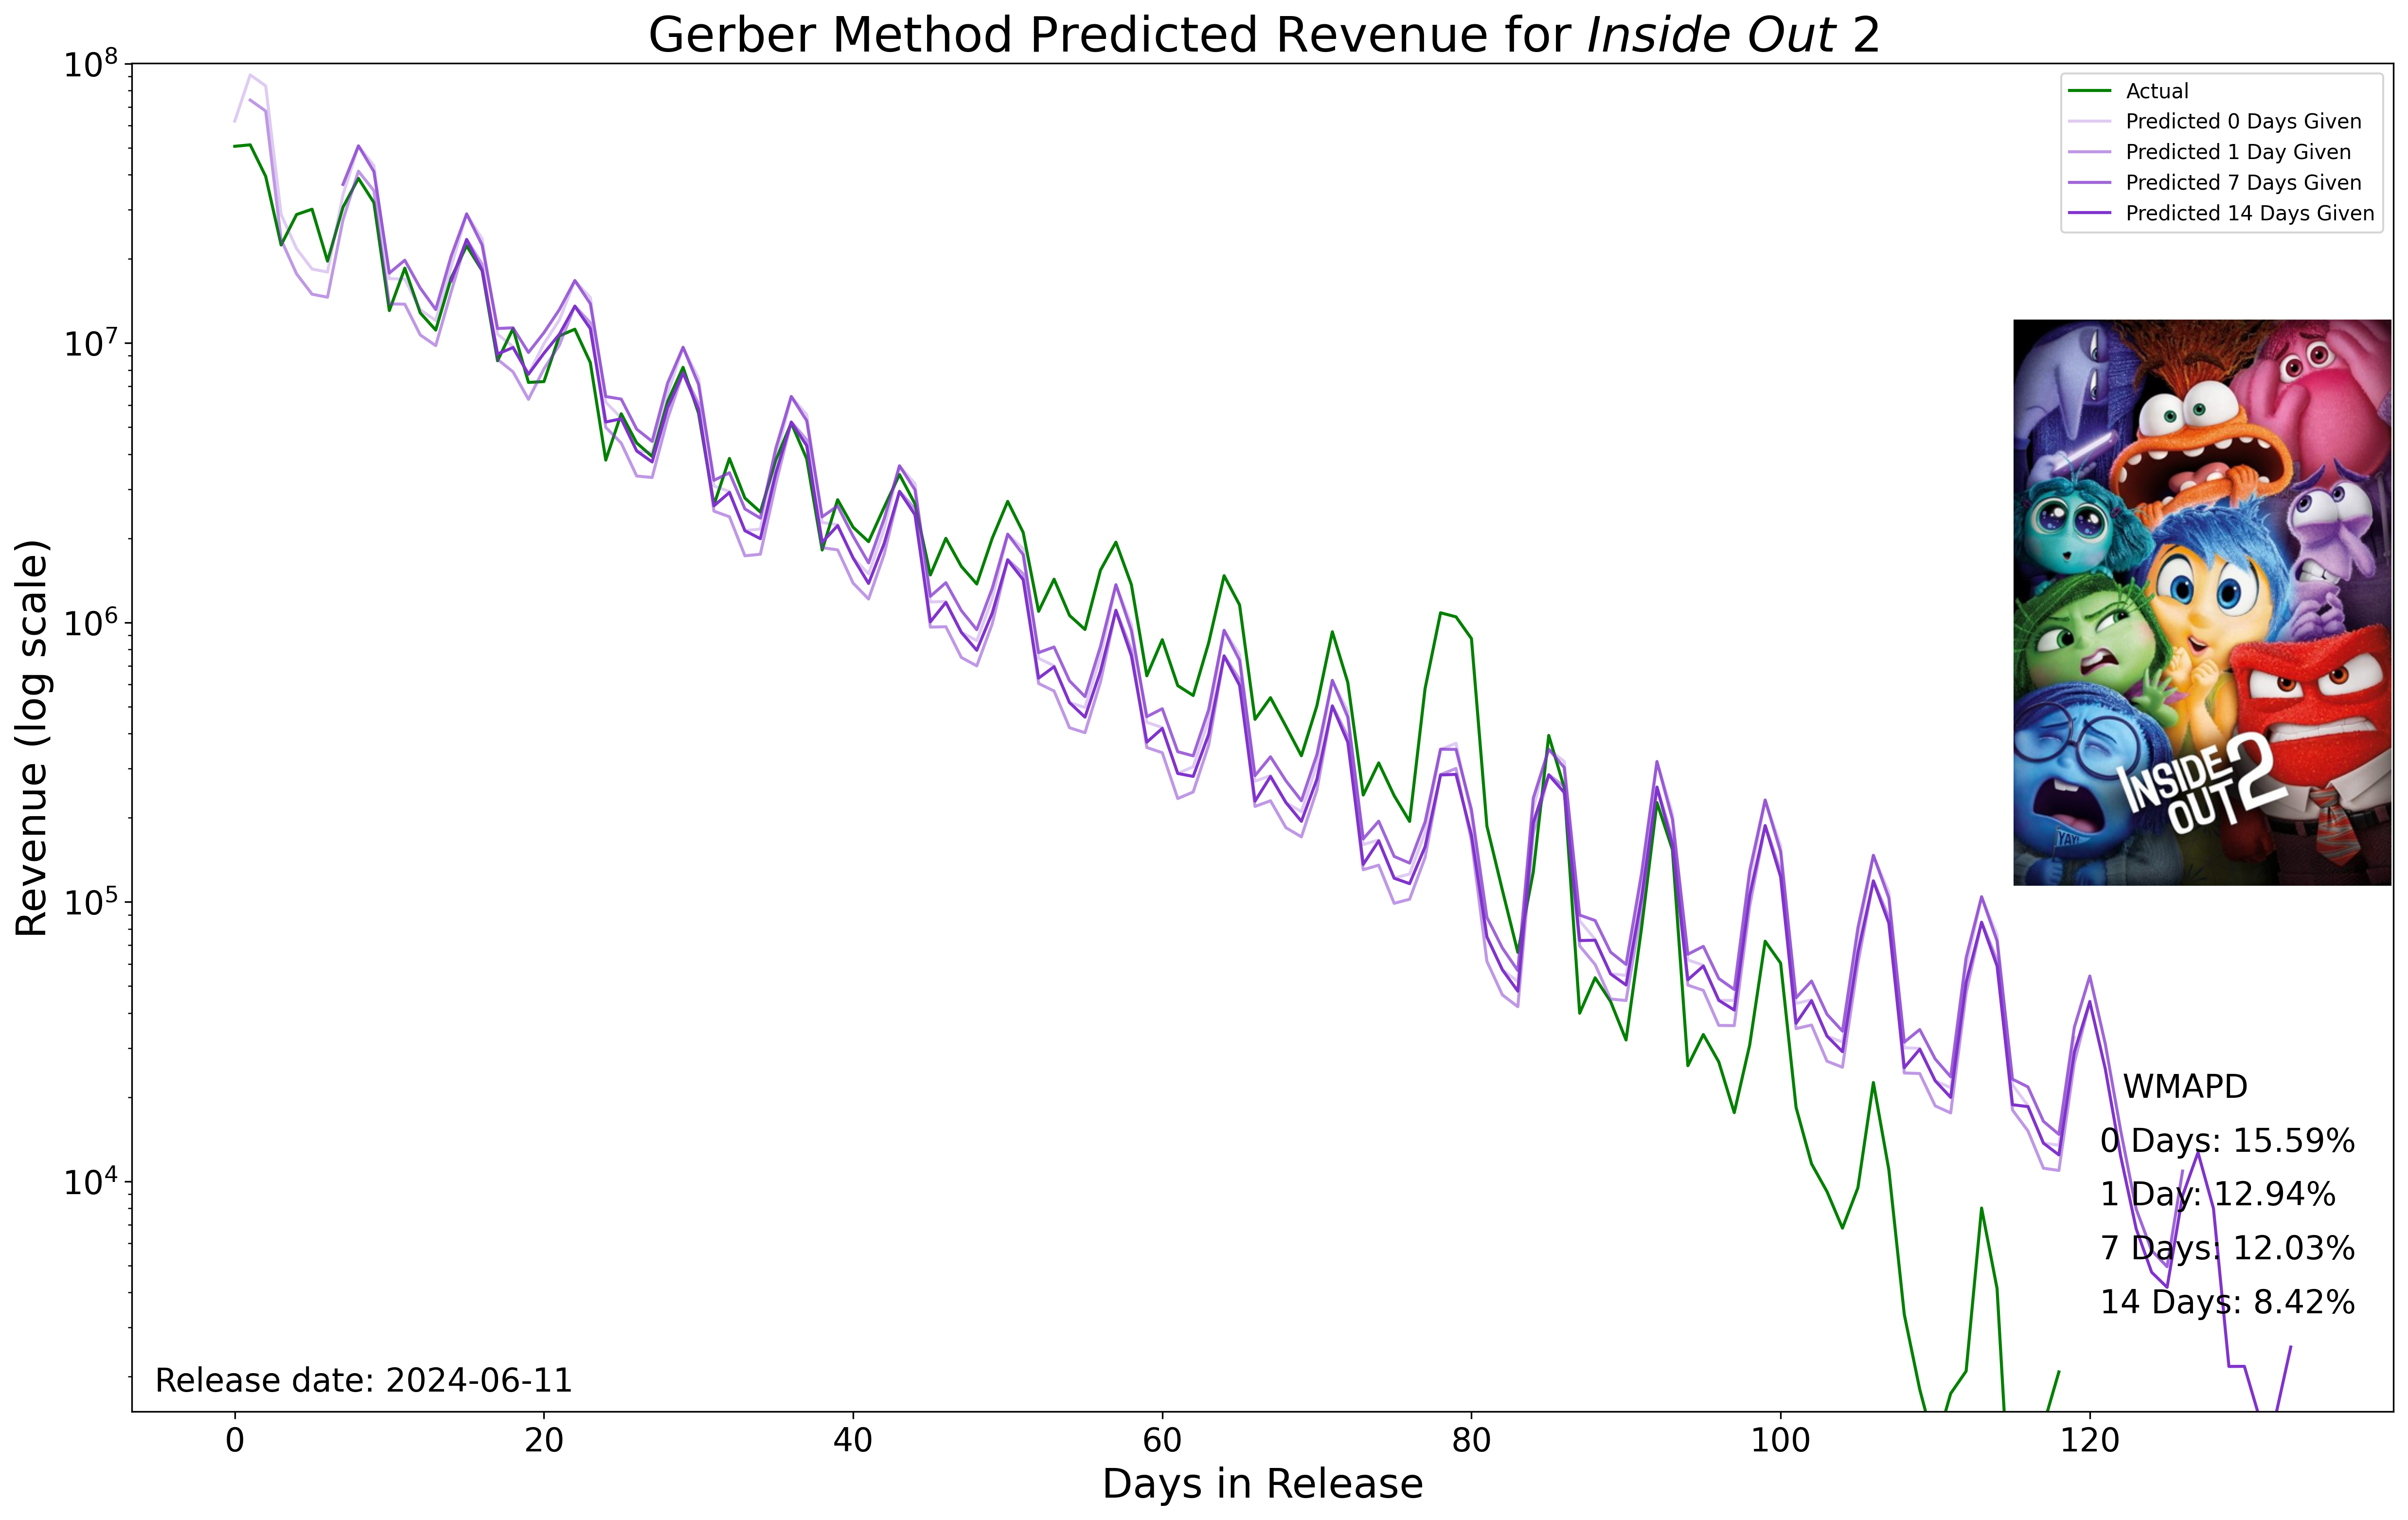
\includegraphics[width=0.769\textwidth]{../shared/images/pred/Inside Out 2_multiple_4.png}
    \caption{This plot presents predictions for \cite{insideOut2} given 0, 1, 7, and 14 days.}
    \label{fig:predinsideout}
\end{figure}

\textit{Inside Out 2} was the highest grossing movie of 2024 and the highest animated grosser of all time \citep{insideOut2Profits}. The model performs well in predicting this outlier case. The opening day prediction is reasonably accurate and then when the model is given 2 weeks of data, its performance improves significantly based on higher weekly multipliers.

Finally, we can see the results for \cite{meanGirls} in Figure \ref{fig:predmeangirls}.

\begin{figure}[H]
    \centering
    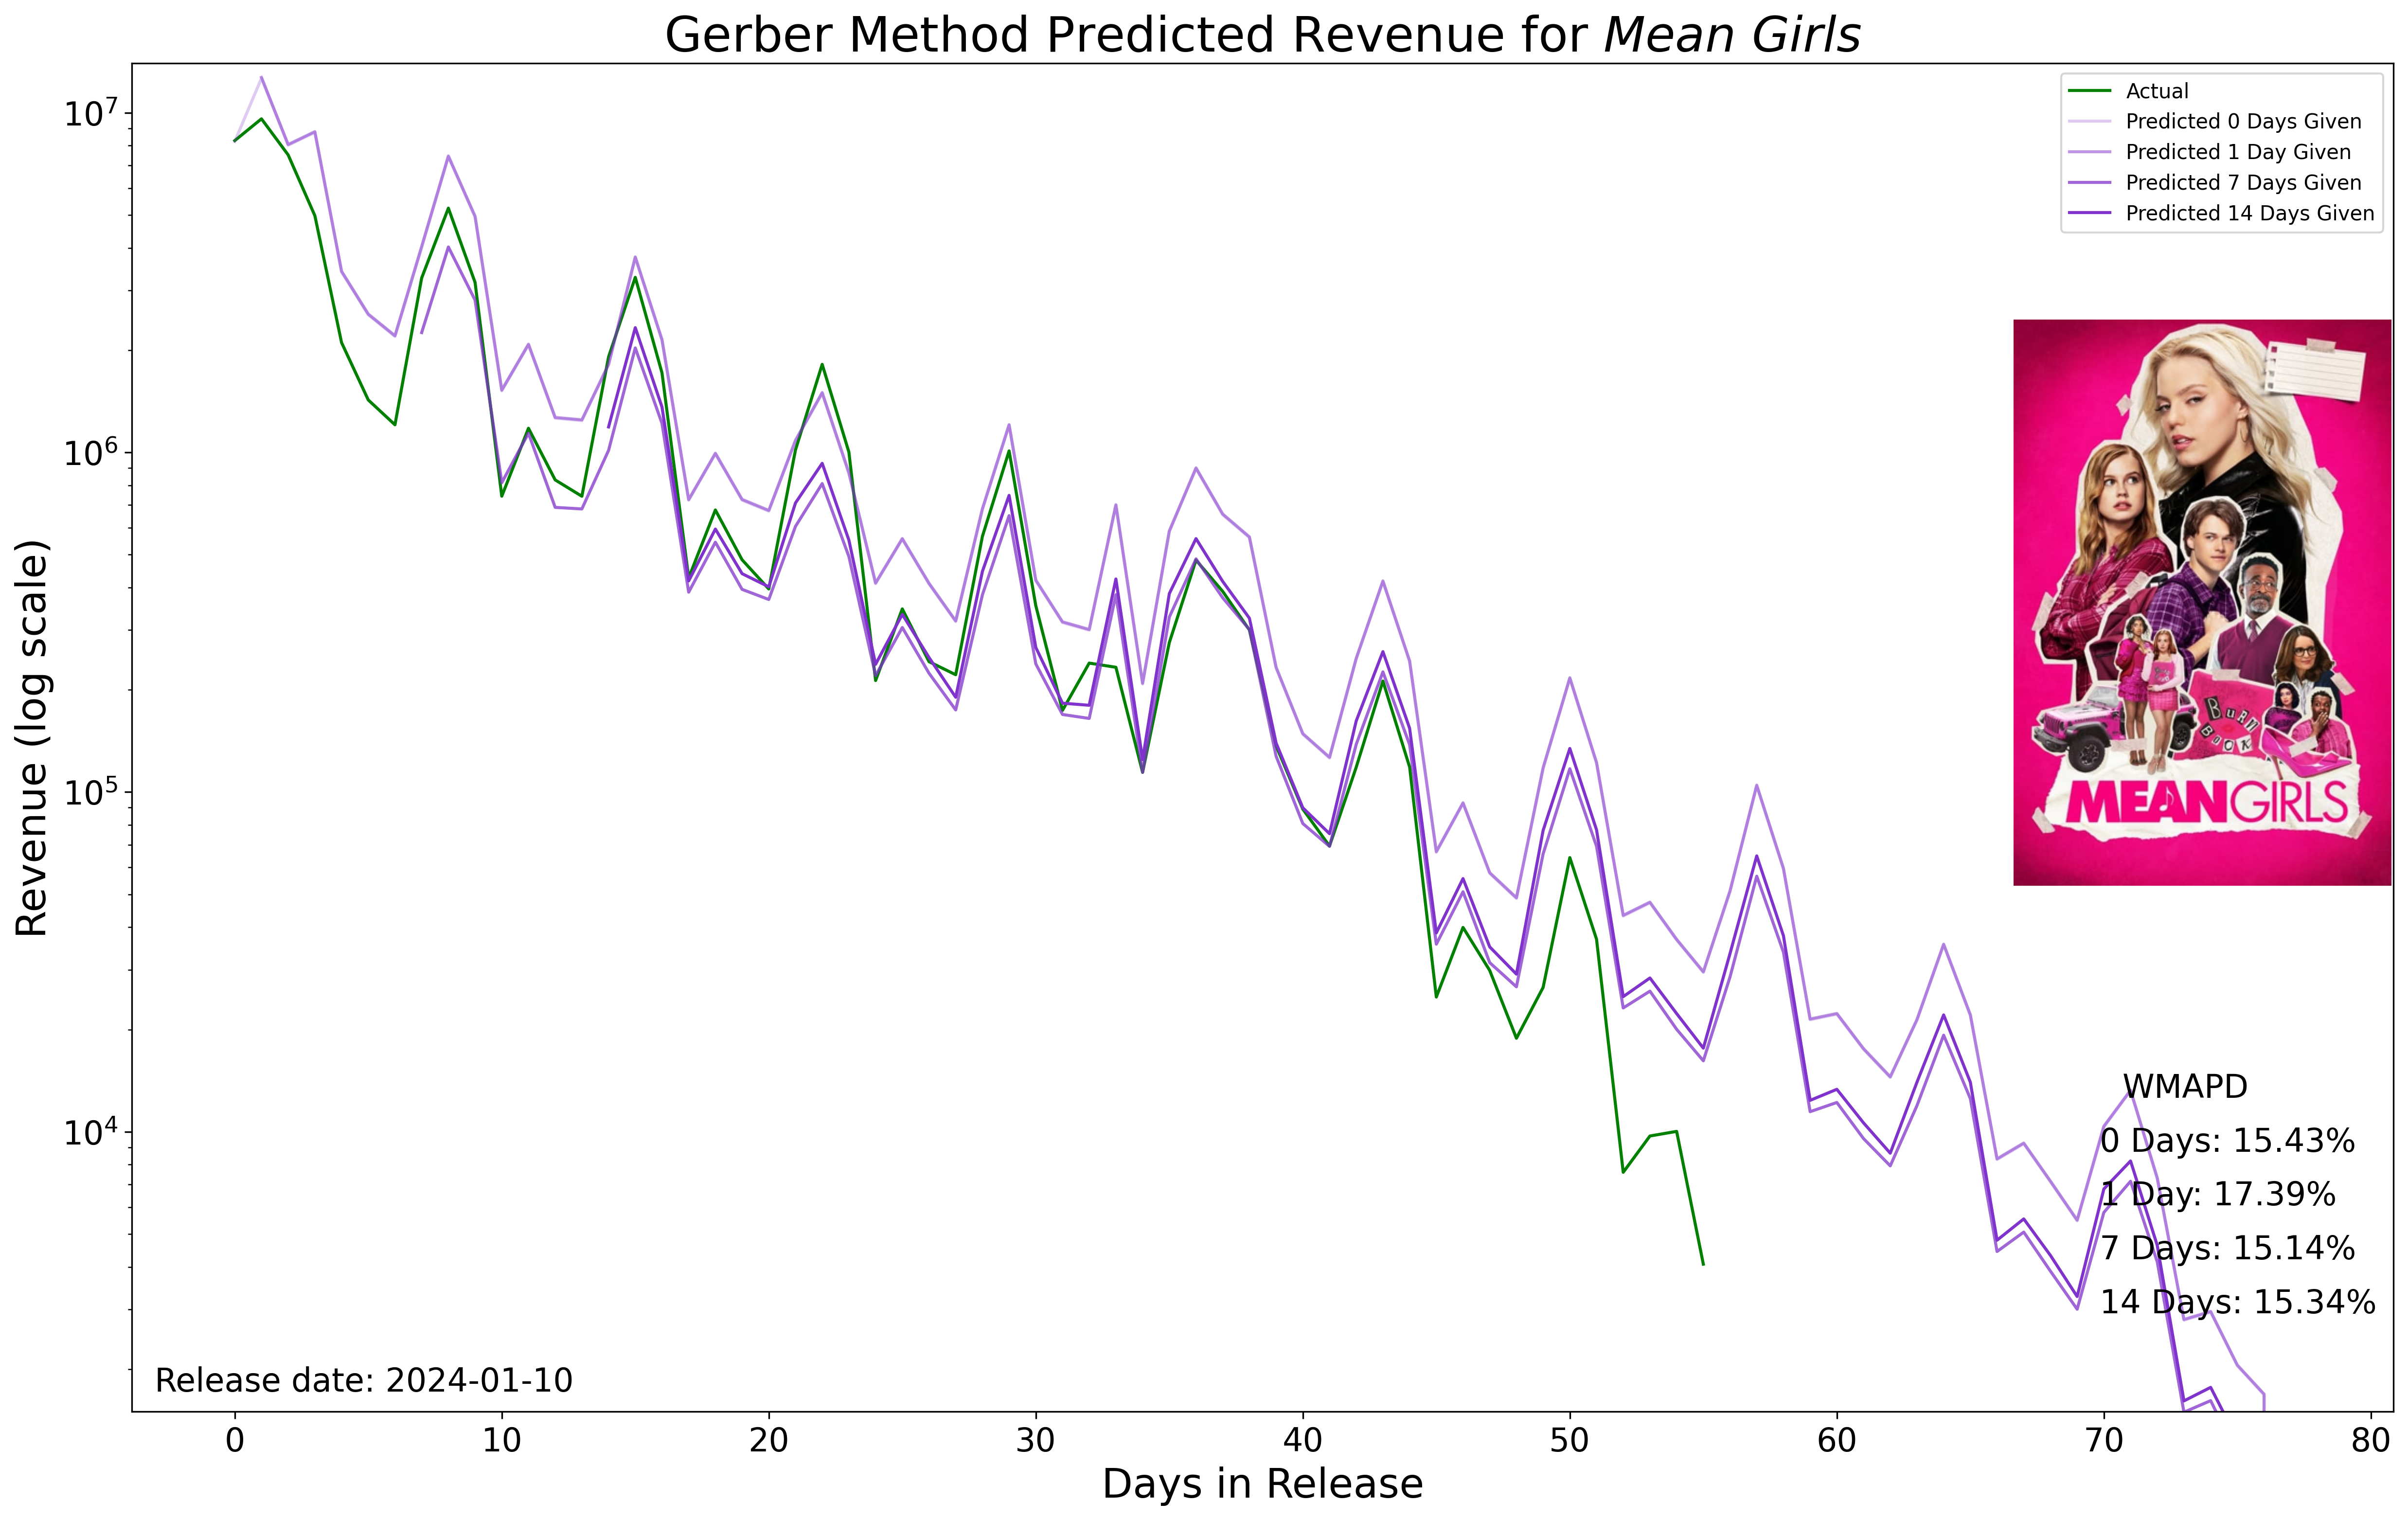
\includegraphics[width=0.769\textwidth]{../shared/images/pred/Mean Girls_multiple_4.png}
    \caption{This plot presents predictions for \cite{meanGirls} given 0, 1, 7, and 14 days.}
    \label{fig:predmeangirls}
\end{figure}

This case is interesting because the opening day prediction was nearly perfect. This means that the series given 0 days and given 1 day are nearly identical. Eventually, \textit{Mean Girls} trends away from initial expectations and the predictions given 7 and 14 days update to reflect this trend.

In the appendix are more examples for \cite{alienRomulus} (Figure \ref{fig:predalienmulti}), \cite{anora} (Figure \ref{fig:predanora}), \cite{captainAmerica} (Figure \ref{fig:predbrave}), \cite{paddingtonPeru} (Figure \ref{fig:predpaddington}), \cite{reagan} (Figure \ref{fig:predreagan}), \cite{terrifier3} (Figure \ref{fig:predterrifier3}), \cite{transformersOne} (Figure \ref{fig:predtransformersmulti}), and \cite{wildRobot} (Figure \ref{fig:predwildrobot}) over a variety of days given.

\section{Discussion} \label{sec:discussion}

The primary goal of this paper was to develop a model that predicts the daily box office gross of a movie domestically. We present a novel method for utilizing multipliers based on programmatic comps. A key finding is that this strategy is effective. Despite the limited information the model is given — just movie details, release dates, and opening day gross — the results are robust.

These results are important because they set a new standard to build upon for predicting daily box office. Movies provide a critical cultural influence and are at an interesting intersection between art and business. Even with the rise of streaming, box office remains a critical part of the movie industry. 

Regarding future work, several avenues warrant exploration. A few possible ideas are:

\subsection{Future Work}
\textbf{Awards:} The model does not currently consider awards at all; however, in some cases awards are quite important. For example, we saw earlier in Section \ref{sssec:limitedreleases} that \textit{A Real Pain} had a large spike in box office gross around the time of Oscar nominations. Additionally, \textit{Anora} had a large spike after it won Best Picture. These spikes are not frequent but a few movies every year experience them. One direction to go is for an awards prediction model to be built and then use those predictions to inform long-run box office.

\textbf{Community Sources:} On websites such as \textit{Hollywood Stock Exchange \citep{hsxHome}} and \textit{Polymarket \citep{polymarketHighestGrossing}}, users engage in predicting box office gross. If these predictions are accurately tuned, they could be helpful in augmenting model predictions. They don't predict daily gross directly but total gross or weekend gross predictions can be applied to the model.

\textbf{Competition:} The model does not consider other movies that are in theaters simultaneously. Theoretically, studios should consider competition when releasing movies and all movies would be released into relatively interchangeable competition. However, this isn't always the case as seen with \cite{missionImpossible} which released slightly before \cite{barbie} and \cite{oppenheimer}. This potentially led to its underperformance \citep{missionImpossible7Letdown}.

\textbf{Drive-Ins:} Drive-ins commonly have double features with two movies from the same studio. These grosses are given half to each movie. What this means is that studios can use a newer popular movie to help \textit{drive} interest in an older film. For instance, Disney used \cite{incredibles2} to help \cite{wrinkleInTime} \citep{driveInGross}. Additionally, drive-ins experienced a resurgence during the COVID-19 pandemic, so they could remain a popular way for people to watch movies \citep{driveInPandemic}. This model does not consider drive-ins at all.

\textbf{Implementing Previews:} Currently, the model considers previews with regards to how they impact the opening day gross. However, it doesn't consider them beyond this initial impact. Previews are a very useful way for the model to more accurately predict opening day and therefore the rest of the time series. Also, if the model was to be implemented for predicting overall box office, it would need to also predict previews.

\textbf{More Complex Seasonal Multipliers:} The seasonal multipliers work quite well but are based on median movies. It is possible that different movies may do better at certain times of the year (such as horror movies in fall or action blockbusters in summer). Therefore, implementing seasonal multipliers that consider the style of movie could be useful.

\textbf{Popularity:} The model utilizes popularity metrics such as Wikipedia page views and YouTube trailer views for opening day predictions but not after that. It would be interesting to see if these metrics are correlated with any aspects of box office gross and whether they could be used to improve the model.

\textbf{Re-Releases:} Popular movies such as \cite{interstellar} and \cite{revengeOfTheSith} have had high-grossing re-releases in recent years \citep{interstellarReRelease, revengeOfTheSithReRelease}. Currently, the model does not differentiate between whether a movie is a re-release or not. Re-releases generally perform differently than original releases, so implementing a more bespoke solution for them would be useful.

\textbf{Reviews and Ratings:} The model does not currently utilize reviews or ratings. This is a useful area for future improvement. One approach involves Cinemascores which are audience surveys done after major releases. Analysis shows that Cinemascores are correlated with box office legs \citep{redditCinemascore}. It would be interesting to see if this extends to Metacritic, IMDb, or TMDB ratings.

\textbf{Special Engagement Movies:} Special engagement movies such as \cite{erasTour} and \cite{renaissance} were very prominent in the 2023 box office and are growing in popularity. These movies frequently release only on Thursdays through Sundays which the model does not currently account for. As special engagement concert movies grow in popularity, it would be useful to implement more options for release schedules if certain movies are not out every day of the week.

\textbf{Visualizations:} The information from the model could provide valuable insights to stakeholders. Publishing this information in a more accessible format such as a publicly accessible website would be very useful. This would include a dashboard with the current predictions for all movies in theaters, as well as being able to search for specific movies and see how the model performed on them.

\subsection{Conclusion}
In conclusion, this paper presents a novel method for predicting daily box office gross using a multipliers-based approach. The model is able to predict the daily box office gross of movies with reasonable accuracy and can be used to inform studios about the expected performance of their movies. The model is flexible and can be adapted to different types of movies and release strategies.

\newpage

% References
\bibliographystyle{../shared/asa}  % Using asa.bst for this style
\bibliography{../shared/refs}

\newpage
\appendix

\section{Appendix} \label{sec:appendix}

\begin{figure}[H]
    \centering
    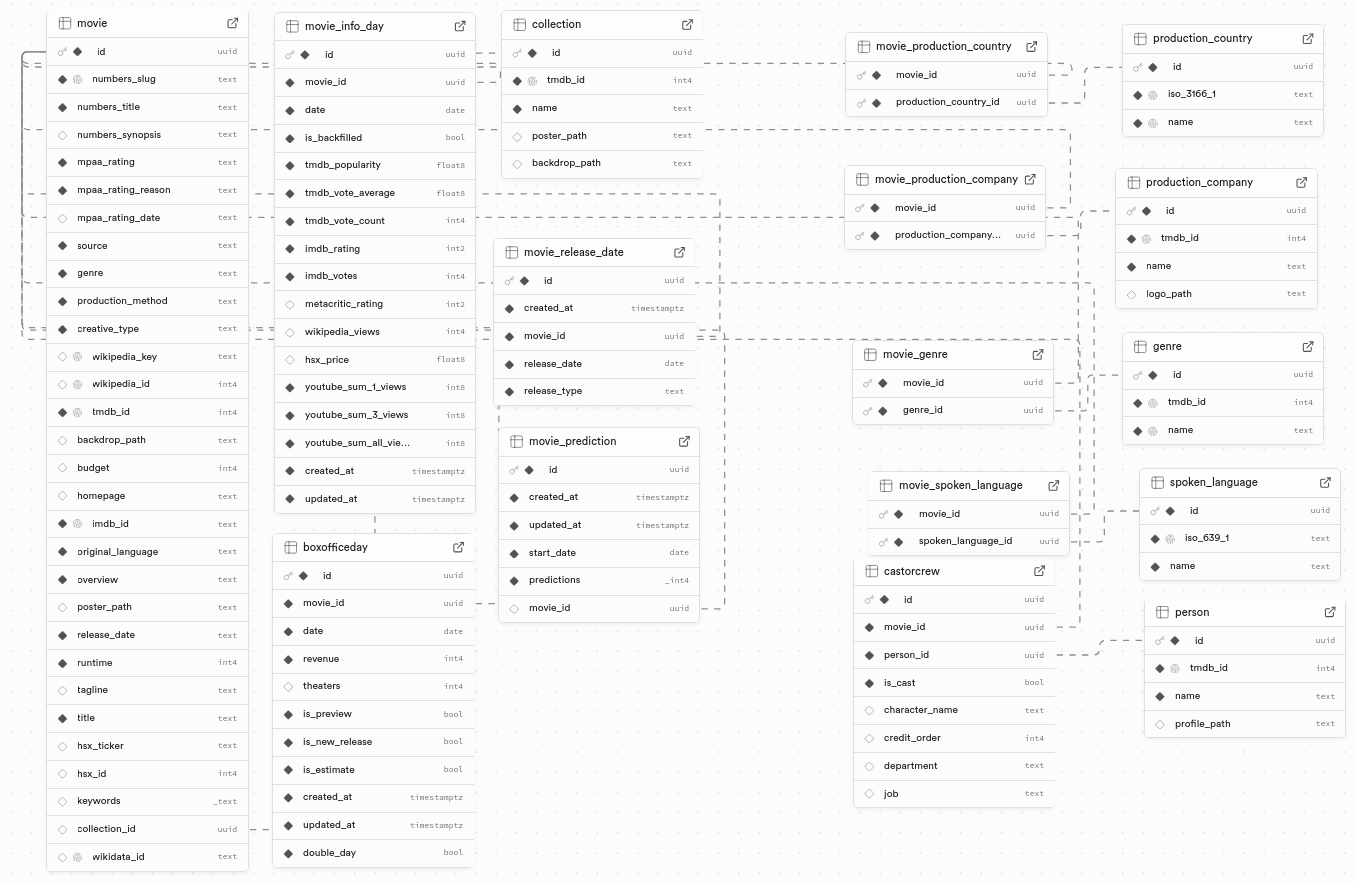
\includegraphics[width=0.8\textwidth]{../shared/images/database.png}
    \caption{This figure showcases the different database uses a visualization tool in Supabase. These are a variety of different tables but the most critical are movie, movie info day, and boxofficeday. The movie table contains the basic information about the movie such as title, release date, and budget. The movie info day table contains the daily information about the movie such as wikipedia views, imdb rating, and youtube views. The boxofficeday table contains the daily box office gross for the movie. The other tables are used for linking information such as cast and crew, production companies, and genres. The difference between the movie info day and boxofficeday tables is that the movie info day table contains information about the movie that is not directly related to box office gross and therefore can occur on days when the movie is not in theaters. The boxofficeday table contains information about the movie that is directly related to box office gross and therefore can only occur on days when the movie is in theaters.}
    \label{fig:database}
\end{figure}

\begin{figure}
    \centering
    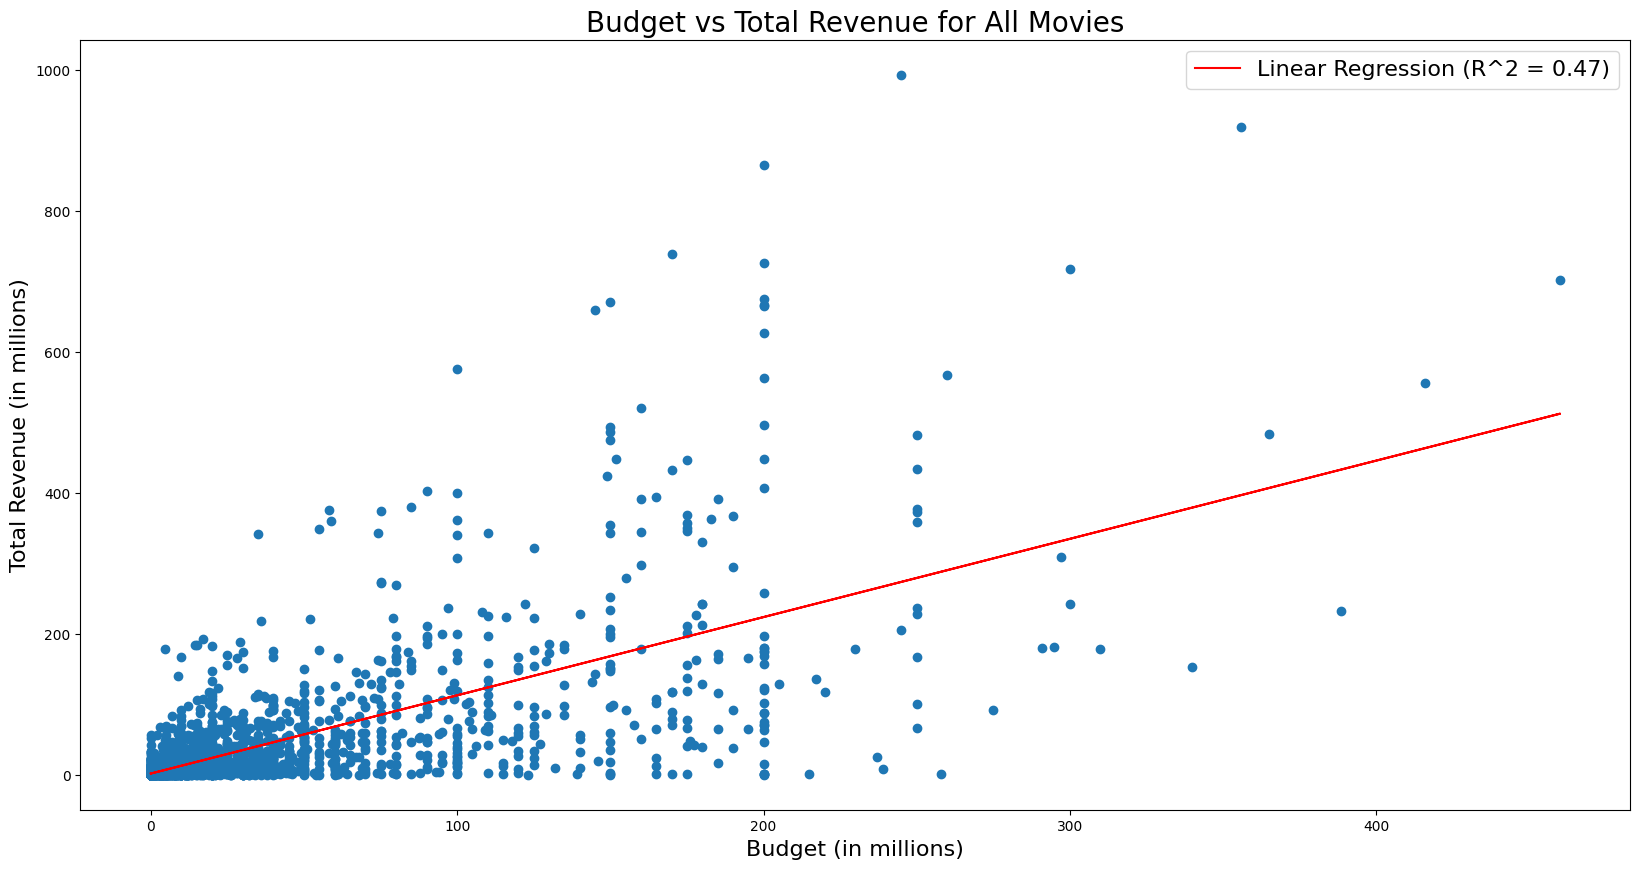
\includegraphics[width=1.0\textwidth]{../shared/images/budgetvsrevenue.png}
    \caption{This plot showcases budget vs revenue for all movies with a linear regression line and a $R^2$ of 0.47. This demonstrates that budget by itself is a very quality predictor of total revenue.}
    \label{fig:budgetvsrevenue}
\end{figure}

\begin{figure}
    \centering
    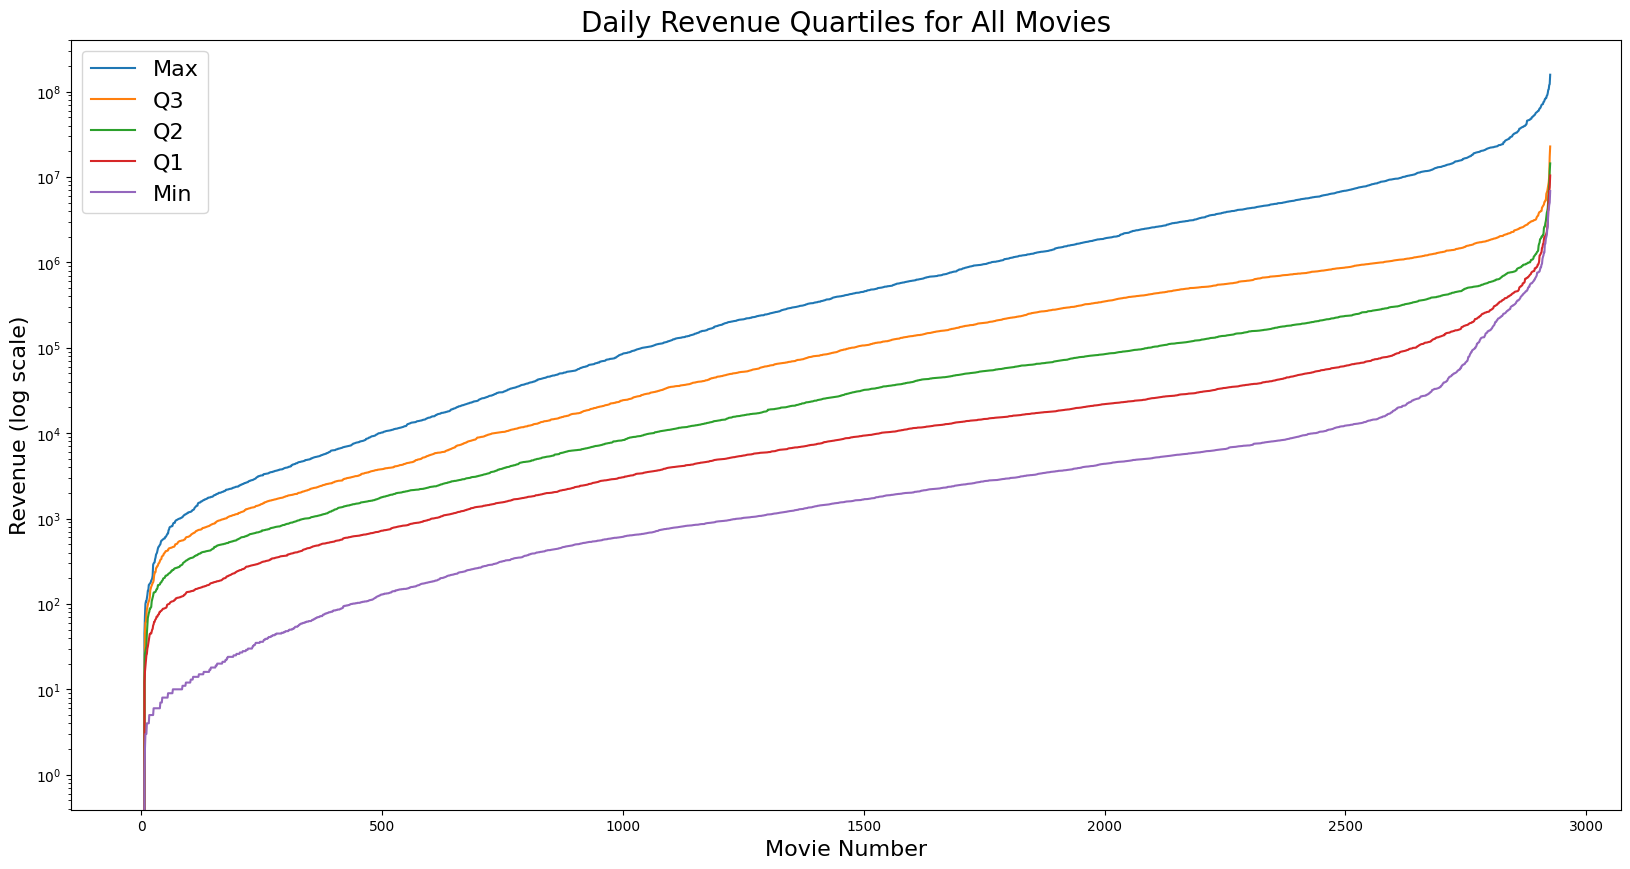
\includegraphics[width=1.0\textwidth]{../shared/images/revenuequartiles.png}
    \caption{This plot showcases the quartiles of daily revenue for all movies. The x-axis is the movie number and the y-axis is the daily revenue on a log scale. There are 5 series for min, 25th percentile, median, 75th percentile, and max. The plot highlights that the largest movies generally have larger minimum grosses which means they leave theaters while making more money. Additionally, the slopes of the lines move smoothly down which demonstrates that there's a somewhat varied set of grosses among movies.}
    \label{fig:revenue}
\end{figure}

\begin{figure}
    \centering
    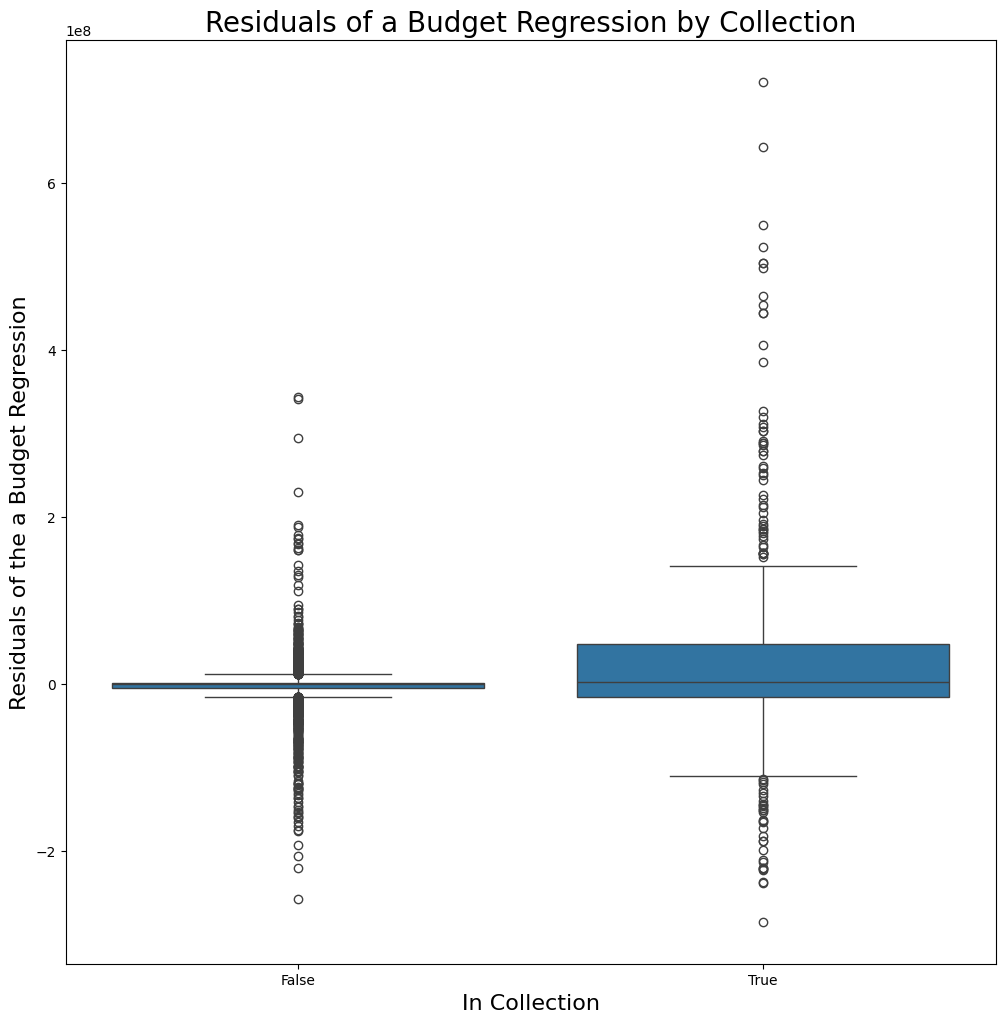
\includegraphics[width=1.0\textwidth]{../shared/images/budgetandcollection.png}
    \caption{These side by side box plots showcase the residuals of a linear regression model for predicting total revenue based on budget. The left plot is the residuals for the model for movies not in a franchise and the right plot is the residuals for movies in a franchise. The residuals are significantly larger in the positive direction for movies in a franchise. This demonstrates that movies in a franchise make more money domestically than what is expected based solely on their budget.}
    \label{fig:budgetandcollection}
\end{figure}

\begin{figure}
    \centering
    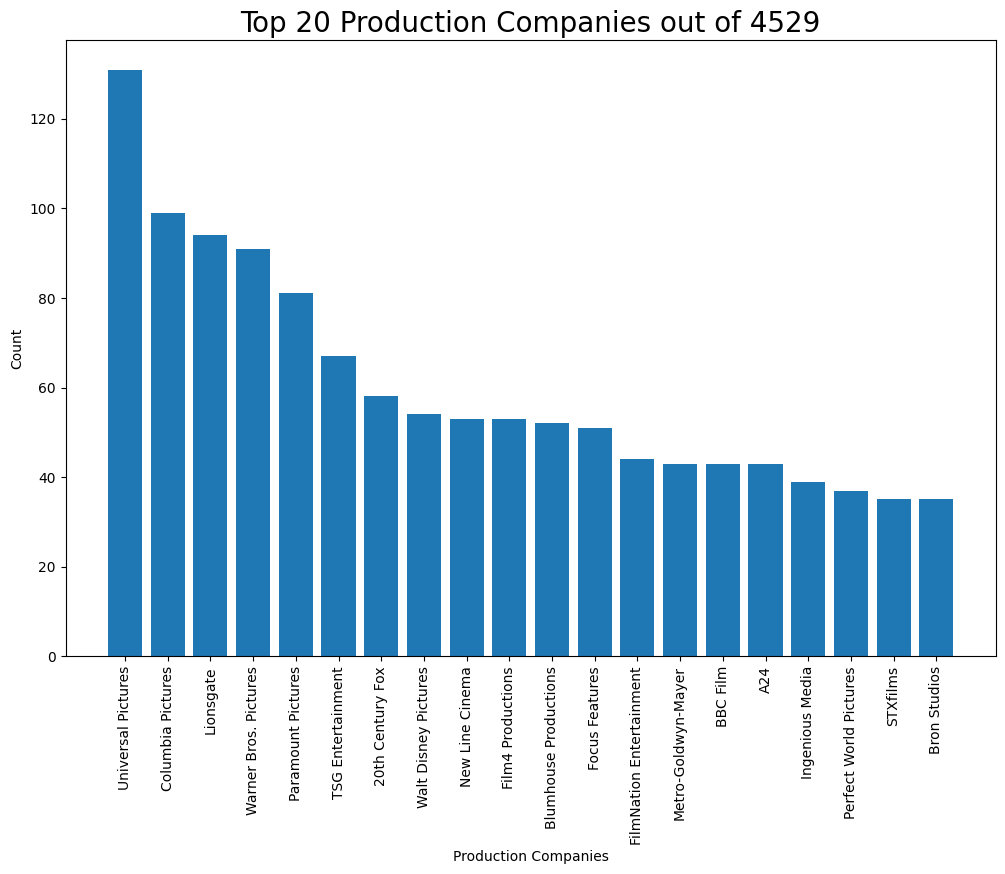
\includegraphics[width=1.0\textwidth]{../shared/images/top20/company.png}
    \caption{This chart showcases the most prominent production companies that release movies to theaters. Universal is the most prolific individual studio with over 120 movies released in the past 10 years. Lots of the big 5 Hollywood studios (Universal, Paramount, Warner Bros, Disney, and Sony) are 5 of the top 7 here. Disney which comes in at \#7 also owns number \#6, 20th Century Fox. Warner Bros (\#4) owns New Line Cinema (\#9).}
    \label{fig:topcompanies}
\end{figure}

\begin{figure}
    \centering
    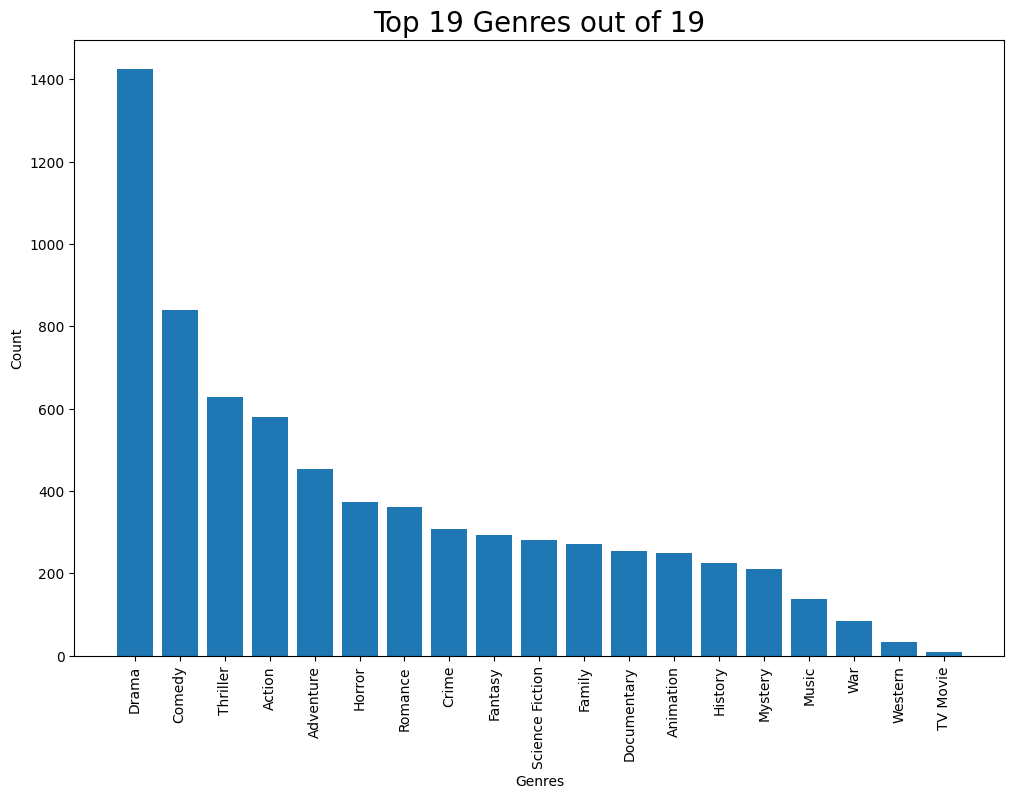
\includegraphics[width=1.0\textwidth]{../shared/images/top20/genre.png}
    \caption{This chart showcases the most prominent genre tags based on TMDB data. Within TMDB, movies can be tagged with many different genres. The most common genre tag is drama by far with 1400 movies having that tag. Comedy, thriller, action, and adventure are not too far behind. Genres such as mystery, music, war, and western are much less common.}
    \label{fig:topgenres}
\end{figure}

\begin{figure}
    \centering
    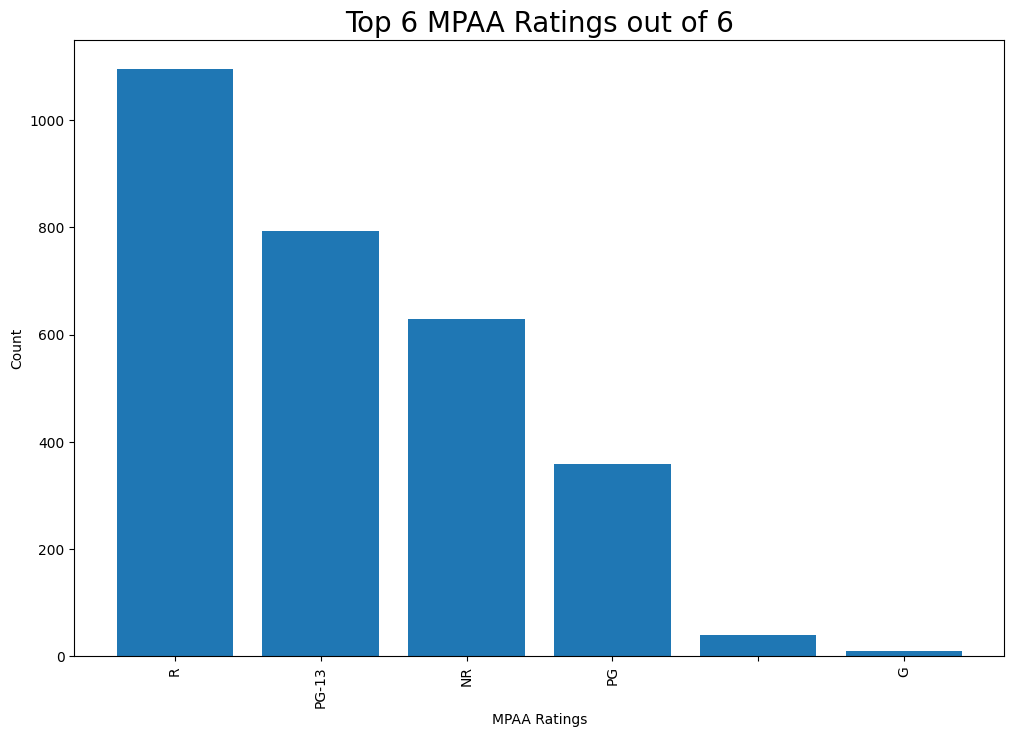
\includegraphics[width=1.0\textwidth]{../shared/images/top20/mpaa.png}
    \caption{These are the top 6 MPAA ratings for movies released in theaters. The most common ratings are R, PG-13, NR, and PG. Then there's a big drop off before no data and finally G. The NR rating is used for movies that are not rated by the MPAA. This is most common for independent movies and documentaries. There are no NC-17 movies in the dataset. The closest was \cite{infinityPool} which was rated NC-17 originally and on appeal but eventually edited down to an R rating \citep{infinityPoolRated}.}
    \label{fig:topmpaa}
\end{figure}

\begin{figure}
    \centering
    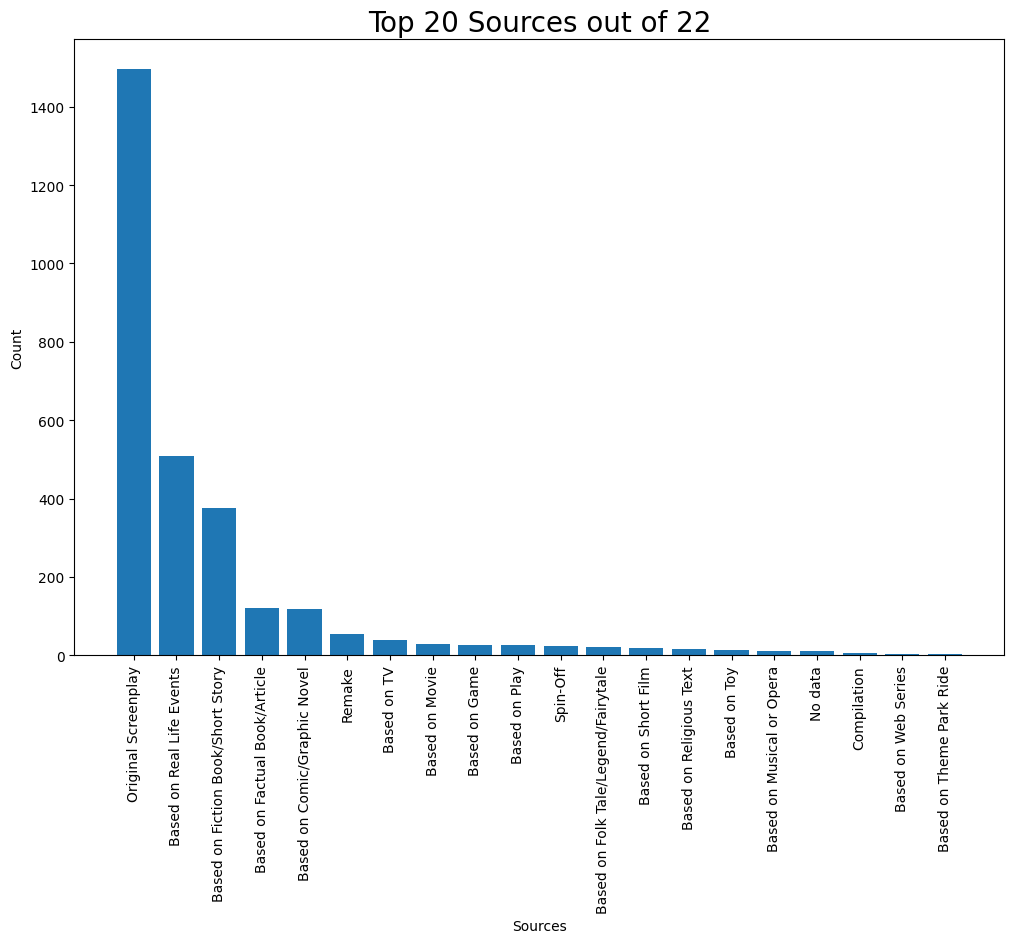
\includegraphics[width=1.0\textwidth]{../shared/images/top20/source.png}
    \caption{This chart showcases the most common sources for movies based on categorization from The Numbers. The most popular source is Original Screenplay by a large margin with real life events and book or short story coming in shortly after. Comic book adaptations come in at \#5, remake at \#6 and game at \#7. Comic book and game adaptations have been huge at the box office recently in terms of gross values but not as much by quantity of movies made \citep{willemsSuperhero}.}
    \label{fig:topsources}
\end{figure}

\begin{figure}
    \centering
    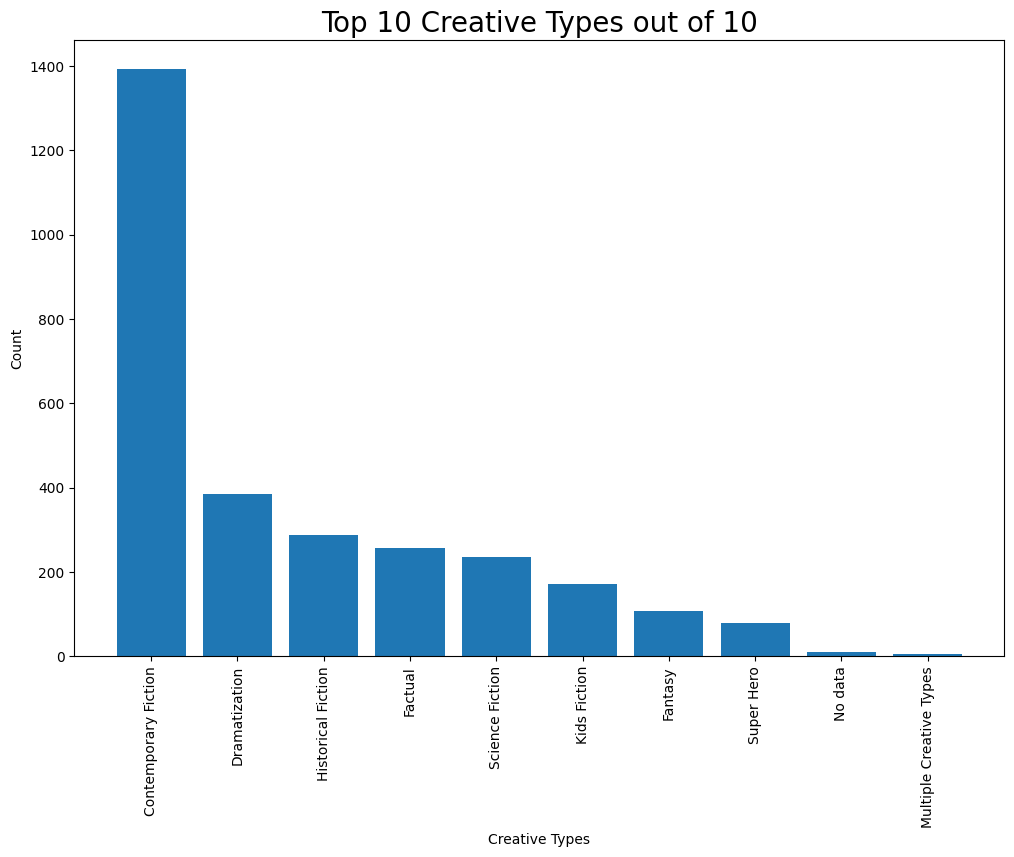
\includegraphics[width=1.0\textwidth]{../shared/images/top20/creative.png}
    \caption{This chart showcases the most common creative types for movies based on categorization from The Numbers. The most popular type is contemporary fiction, then dramatization, and then historical fiction.}
    \label{fig:toptypes}
\end{figure}

\begin{figure}
    \centering
    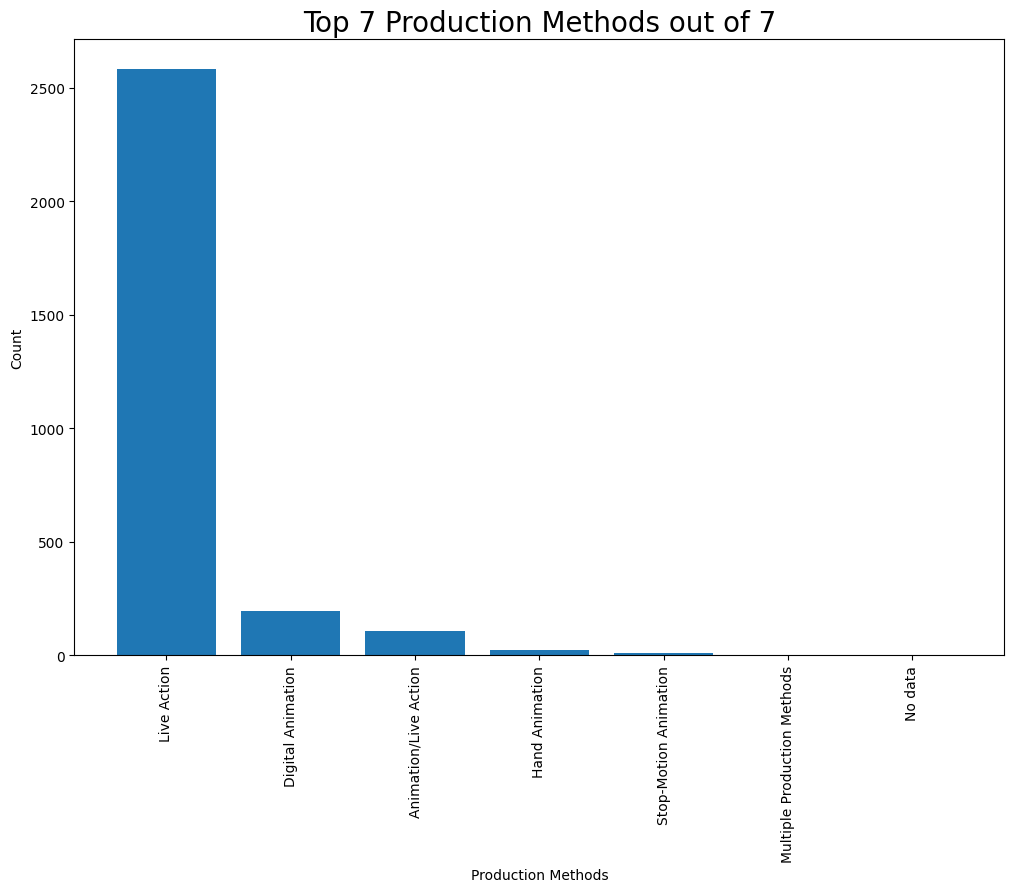
\includegraphics[width=1.0\textwidth]{../shared/images/top20/method.png}
    \caption{This chart showcases the most common production methods. The most popular by far is live action followed by digital animation and animation/live action. Digital animation includes movies we would traditionally think of as animated such as \cite{insideOut2} and \cite{superMario}. Animation/live action includes movies that are live action but feature extensive visual effects and CGI such as \cite{avatarWayOfWater} and \citep{spiderMan}.}
    \label{fig:topmethods}
\end{figure}

\begin{figure}
    \centering
    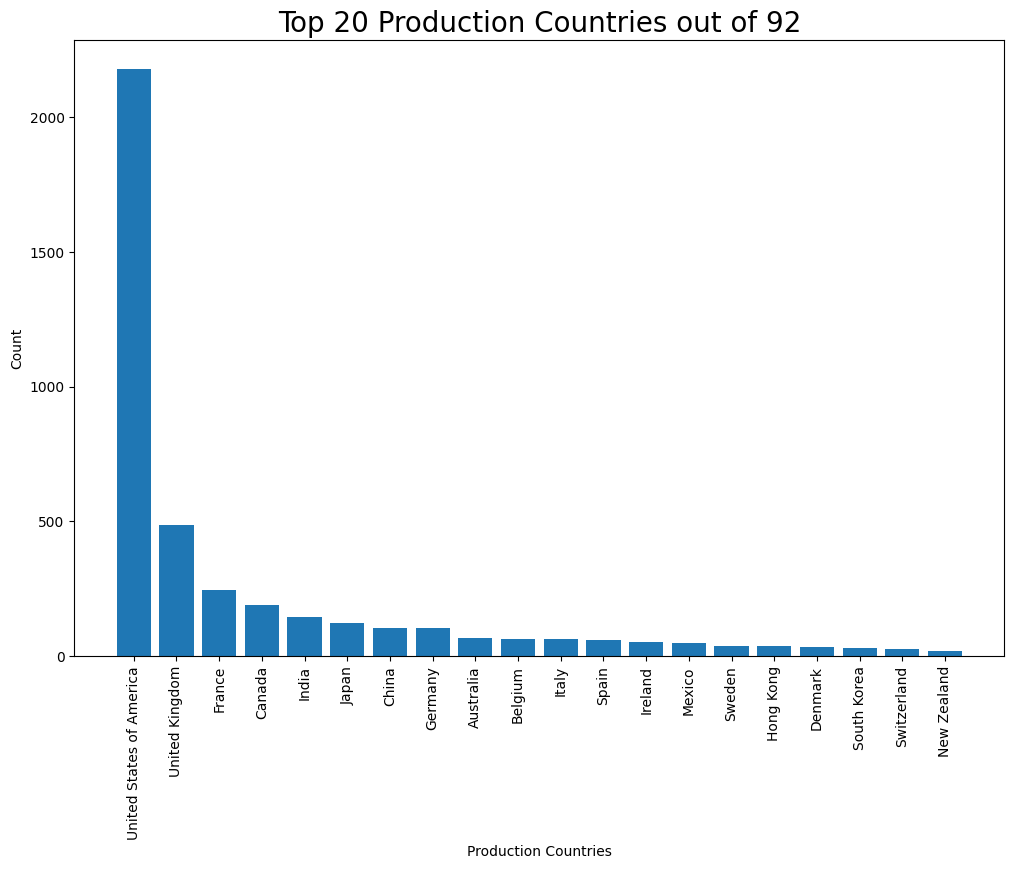
\includegraphics[width=1.0\textwidth]{../shared/images/top20/country.png}
    \caption{This chart showcases the most common production countries. The most common by far is the United States with over 2,000 movies. The next closest is the United Kingdom with nearly 500 movies and after that France, Canada, India, and Japan.}
    \label{fig:topcountries}
\end{figure}

\begin{figure}
    \centering
    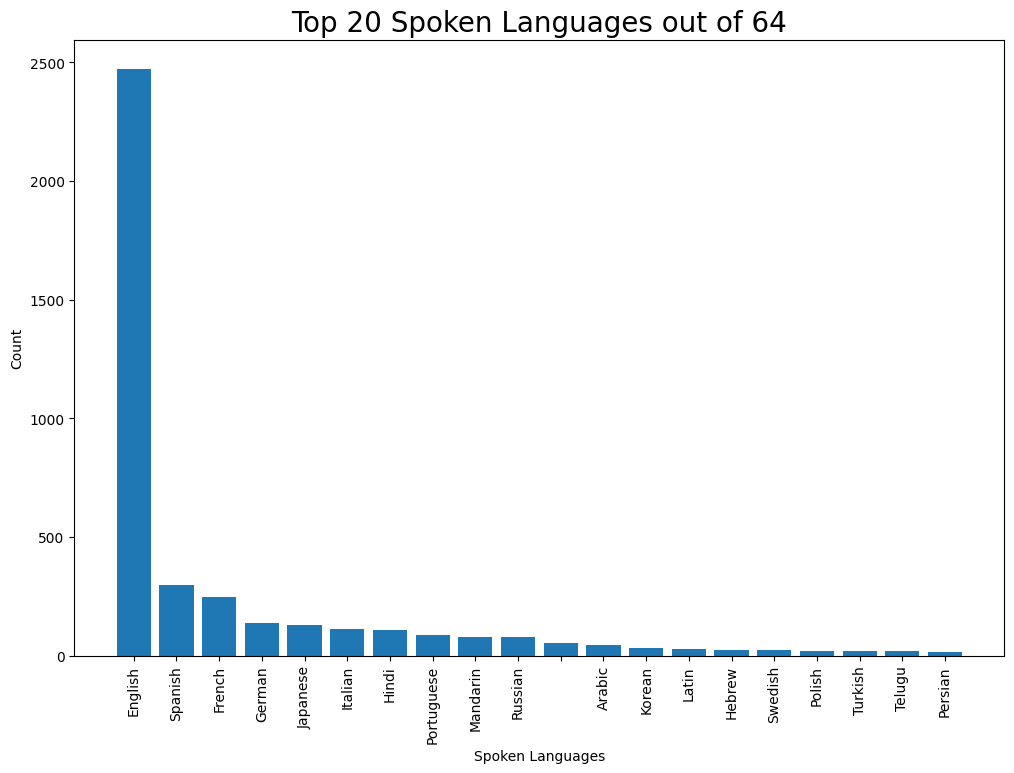
\includegraphics[width=1.0\textwidth]{../shared/images/top20/language.png}
    \caption{This chart showcases the most common production languages. The most common language by far that is spoken in movies released in domestic theaters is English with over 2,000 movies. After that is Spanish, French, German, and Japanese.}
    \label{fig:toplanguages}
\end{figure}

\begin{figure}[H]
    \centering
    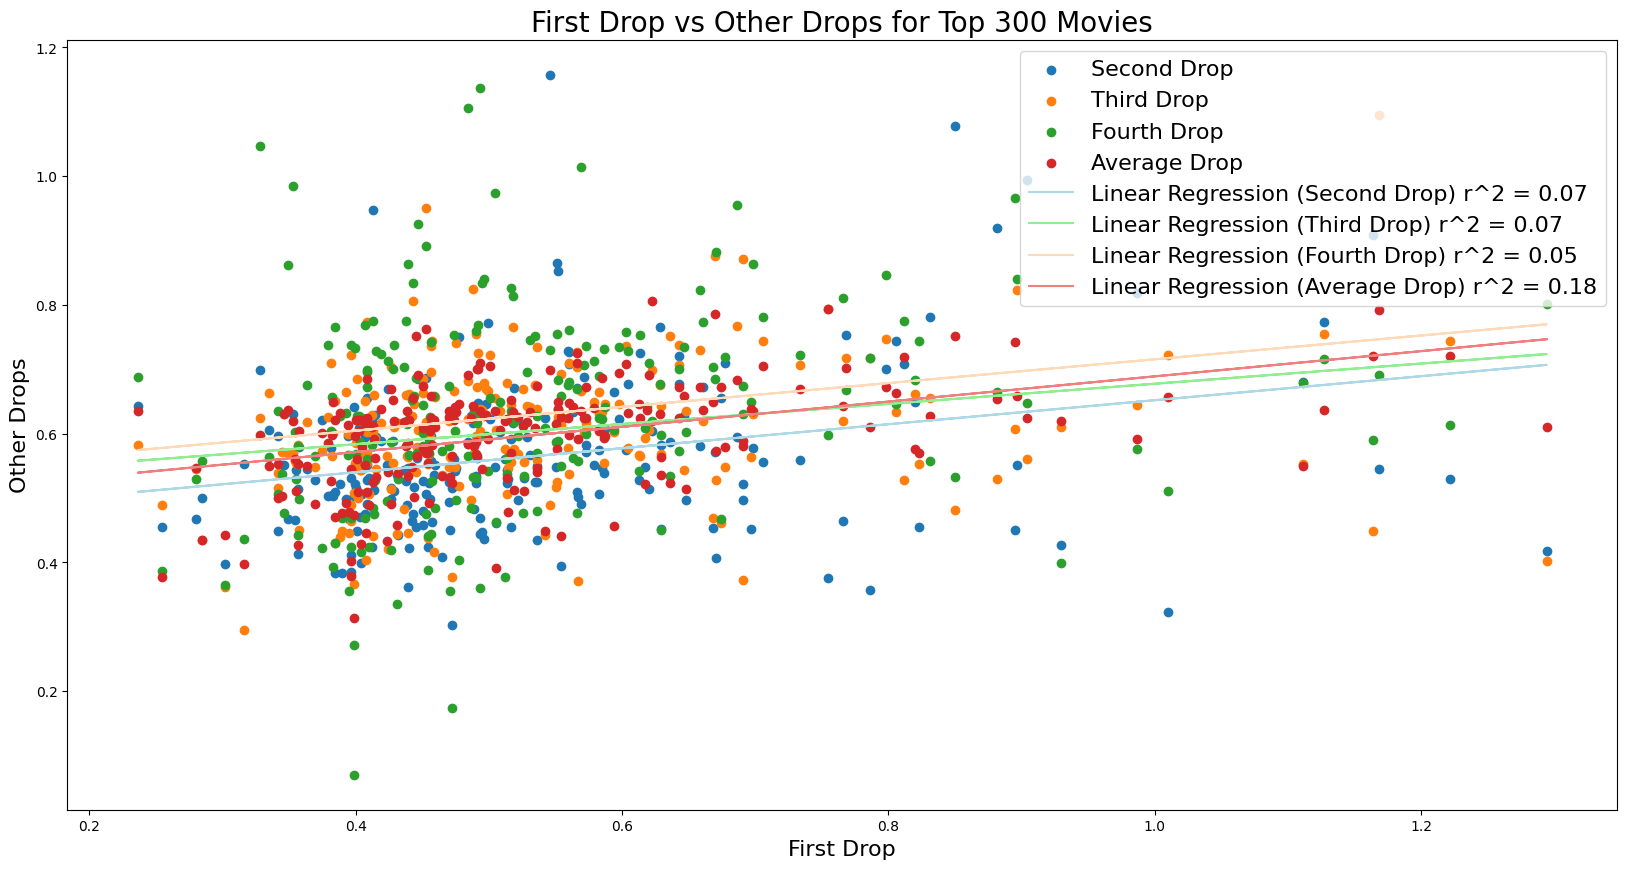
\includegraphics[width=0.7\textwidth]{../shared/images/weeklydrops.png}
    \caption{This plot shows the drop between the first and second week plotted against the drop between the second and third week, third and fourth week, fourth and fifth week, and finally average of all drops. The x-axis is the drop between the first and second week and the y-axis is the other drops. Additionally, regression lines are plotted for each of the 4 series. There are weekly positive correlations for each of the series, with slightly stronger correlations for the average. This demonstrates that past drops for a movie are a useful input for future drops.}
    \label{fig:otherdrops}
\end{figure}

\begin{figure}
    \centering
    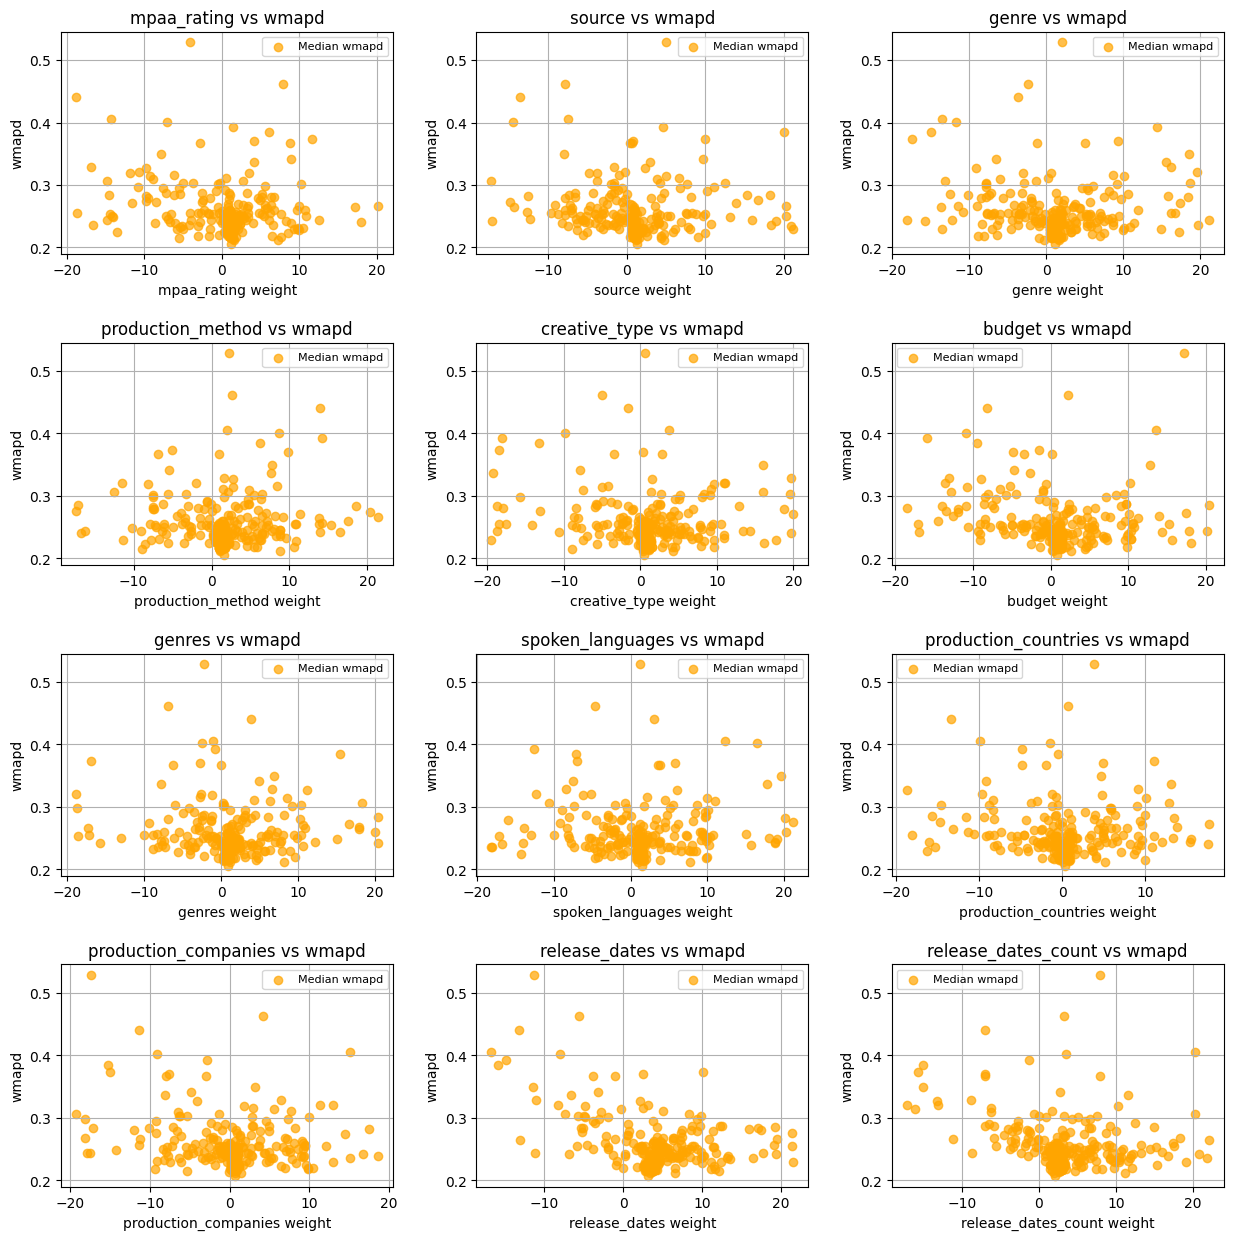
\includegraphics[width=1.0\textwidth]{../shared/images/randomizedgridsearch.png}
    \caption{This series of plots showcases the median WMAPD value for each of the different KNN hyperparameters. These plots are the results of a randomized grid search procedure where the values are randomized and then model performance is analyzed based on a consistent test set of 200 recent releases.}
    \label{fig:gridsearch}
\end{figure}

\begin{figure}
    \centering
    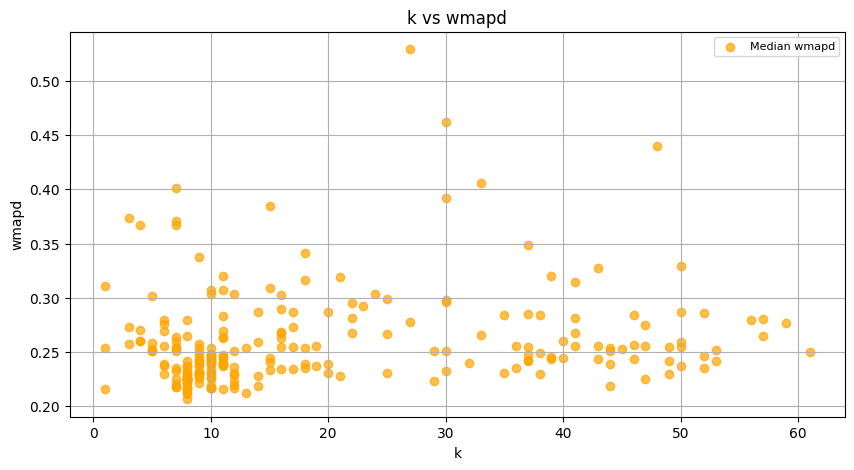
\includegraphics[width=1.0\textwidth]{../shared/images/randomizedgridsearchk.png}
    \caption{Similar to Figure \ref{fig:gridsearch}, this series of plots showcases the median WMAPD value for only the K hyperparameter in KNN. Good results were achieved with a wide variety of K values but the best value ended up being 8 which is what the final model uses.}
    \label{fig:gridsearchk}
\end{figure}

\begin{figure}
    \centering
    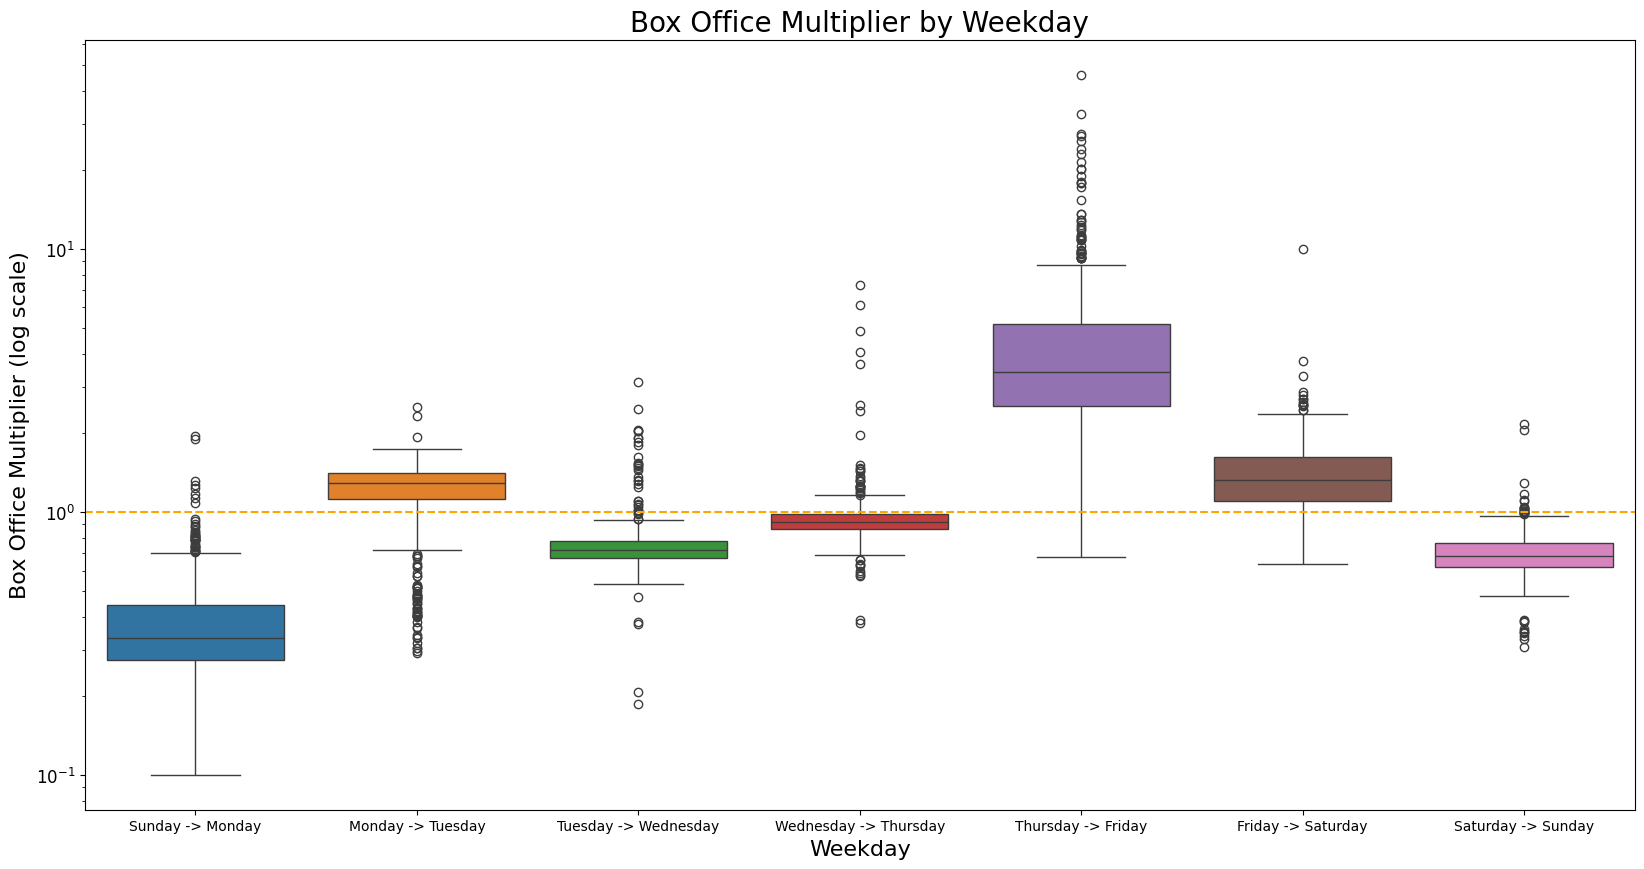
\includegraphics[width=1.0\textwidth]{../shared/images/multbyweekday.png}
    \caption{This series of box plots showcases the box office multiplier based on the day of the week. There is a line at 1 which is no change from previous day. Fridays have the highest multipliers by far. Tuesdays and Saturdays also generally have positive multipliers.}
    \label{fig:multbyweekday}
\end{figure}

\begin{figure}
    \centering
    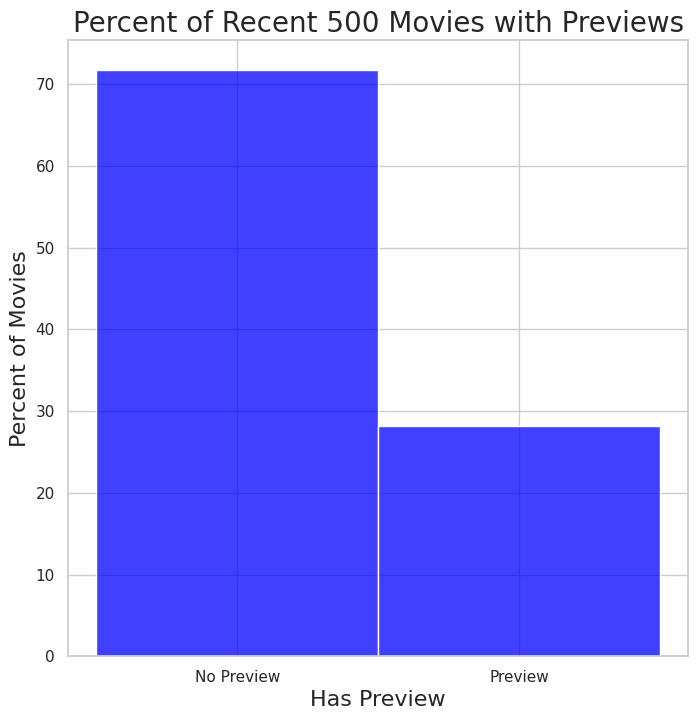
\includegraphics[width=1.0\textwidth]{../shared/images/previewpercent.png}
    \caption{This chart demonstrates the percentage of movies that have previews out of the 500 most recent releases. A bit under 30\% of movies have previews.}
    \label{fig:previewpercent}
\end{figure}

\begin{figure}
    \centering
    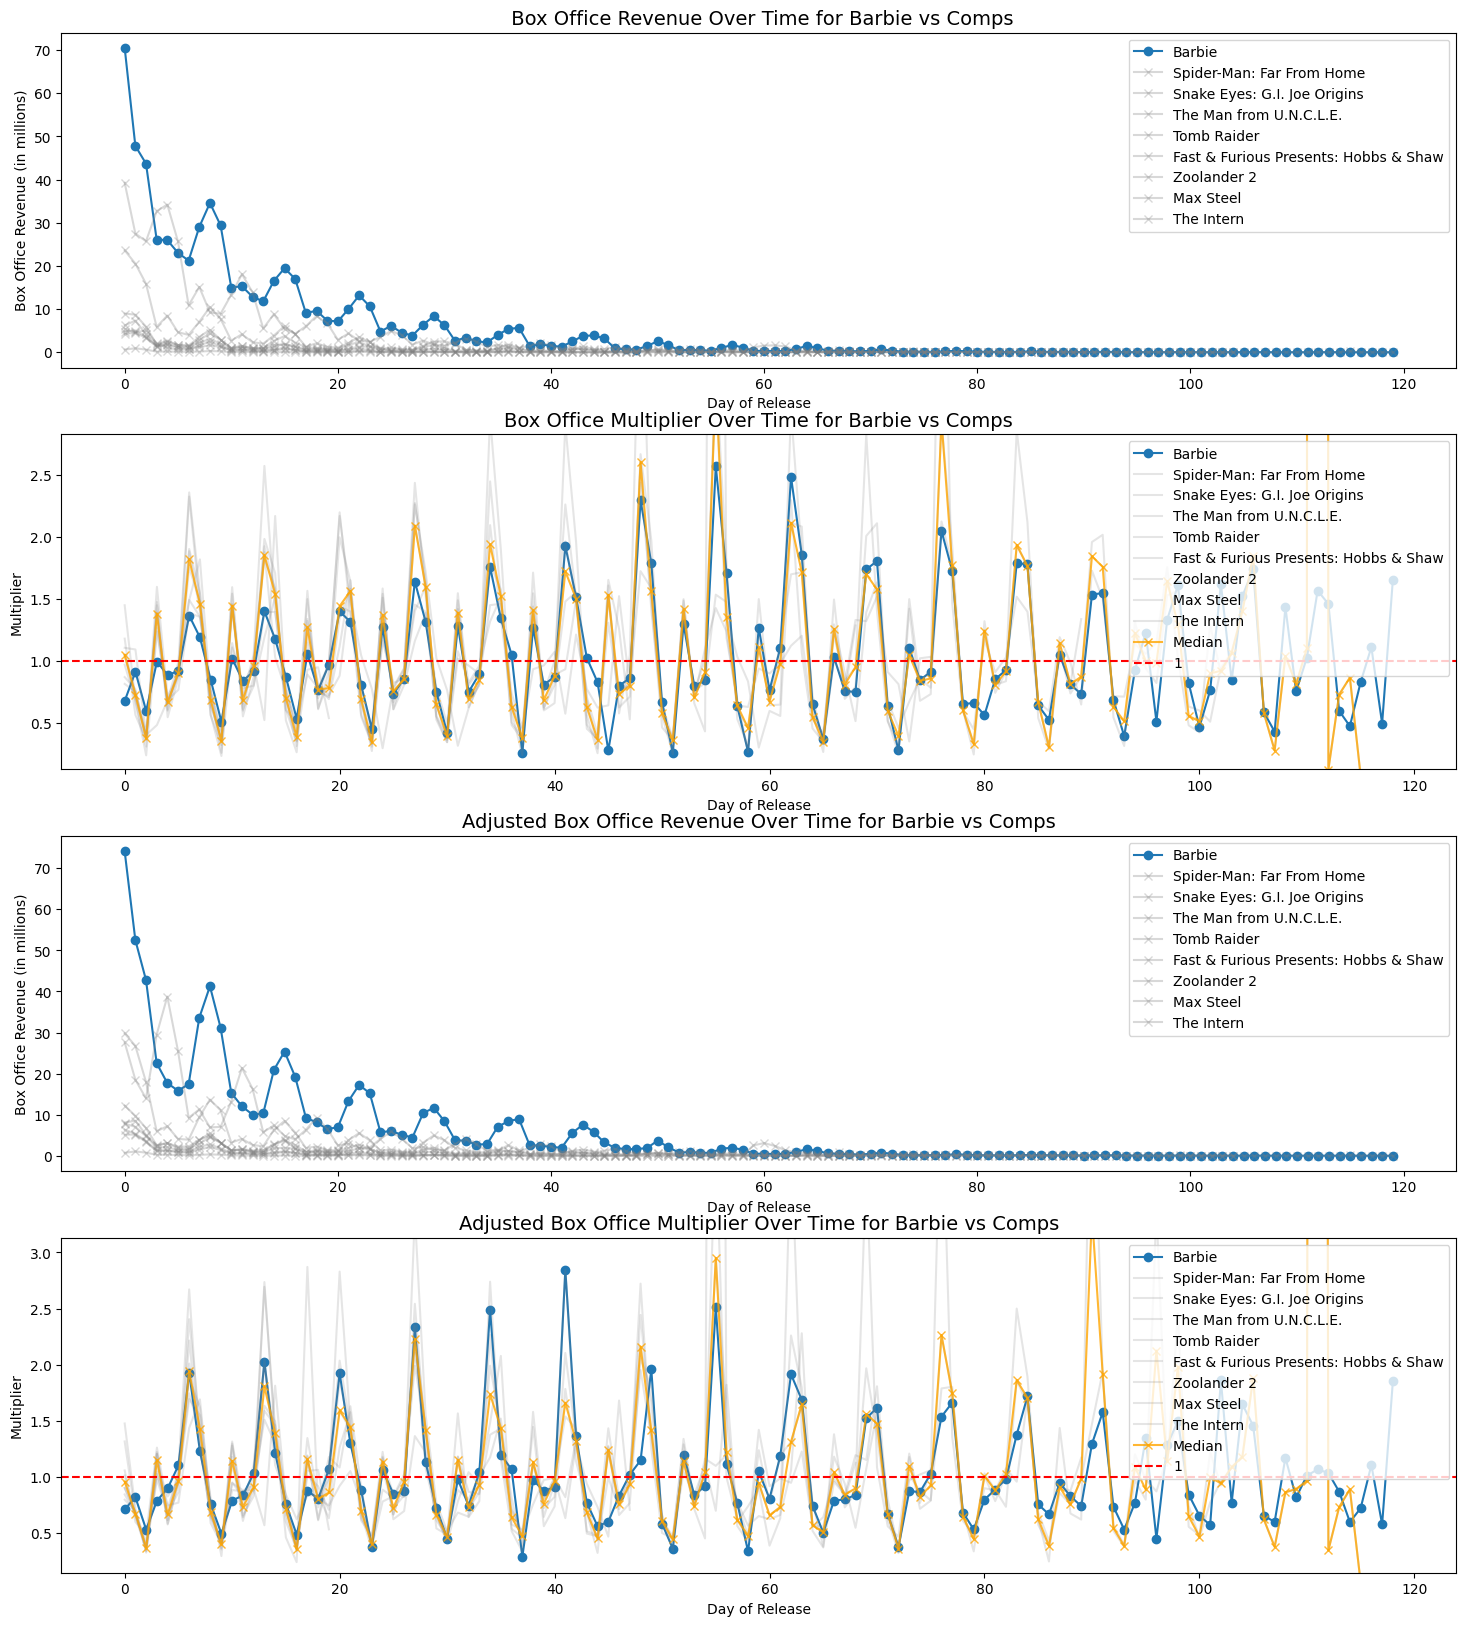
\includegraphics[width=0.9\textwidth]{../shared/images/compsmult/barbie.png}
    \caption{This plot shows comps and multipliers for \cite{barbie}. The top plot is box office revenue for Barbie and each of its comps; the second plot is multipliers for up to 120 days. The next two plots use adjusted gross instead of raw gross. Adjusted gross is based on seasonal and holiday multipliers.}
    \label{fig:compsmultbarbie}
\end{figure}

\begin{figure}
    \centering
    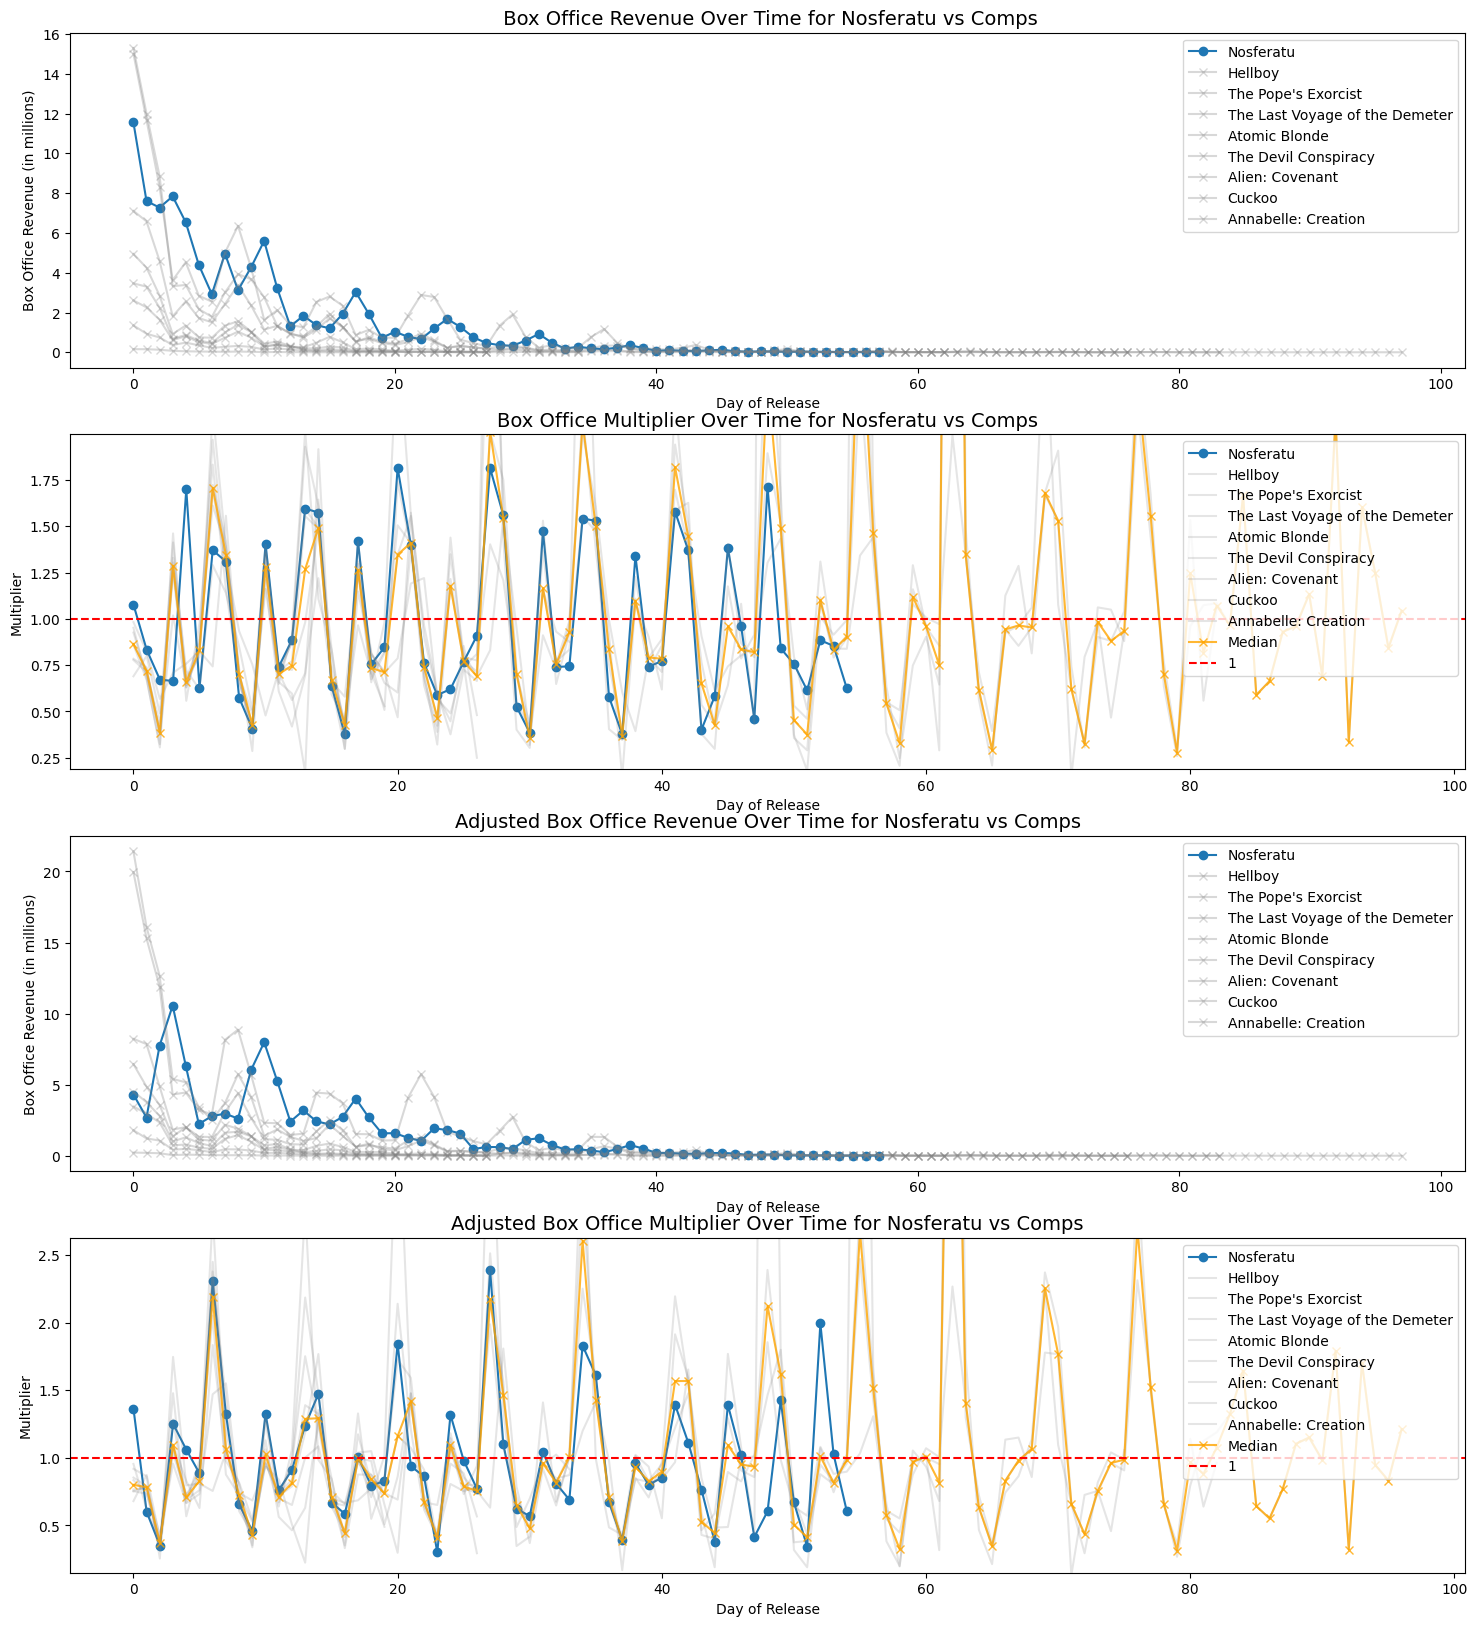
\includegraphics[width=0.9\textwidth]{../shared/images/compsmult/nosferatu.png}
    \caption{This plot shows comps and multipliers for \cite{nosferatu}. The top plot is box office revenue for Nosferatu and each of its comps; the second plot is multipliers for up to 120 days. The next two plots use adjusted gross instead of raw gross. Adjusted gross is based on seasonal and holiday multipliers.}
    \label{fig:compsmultnosferatu}
\end{figure}

\begin{figure}
    \centering
    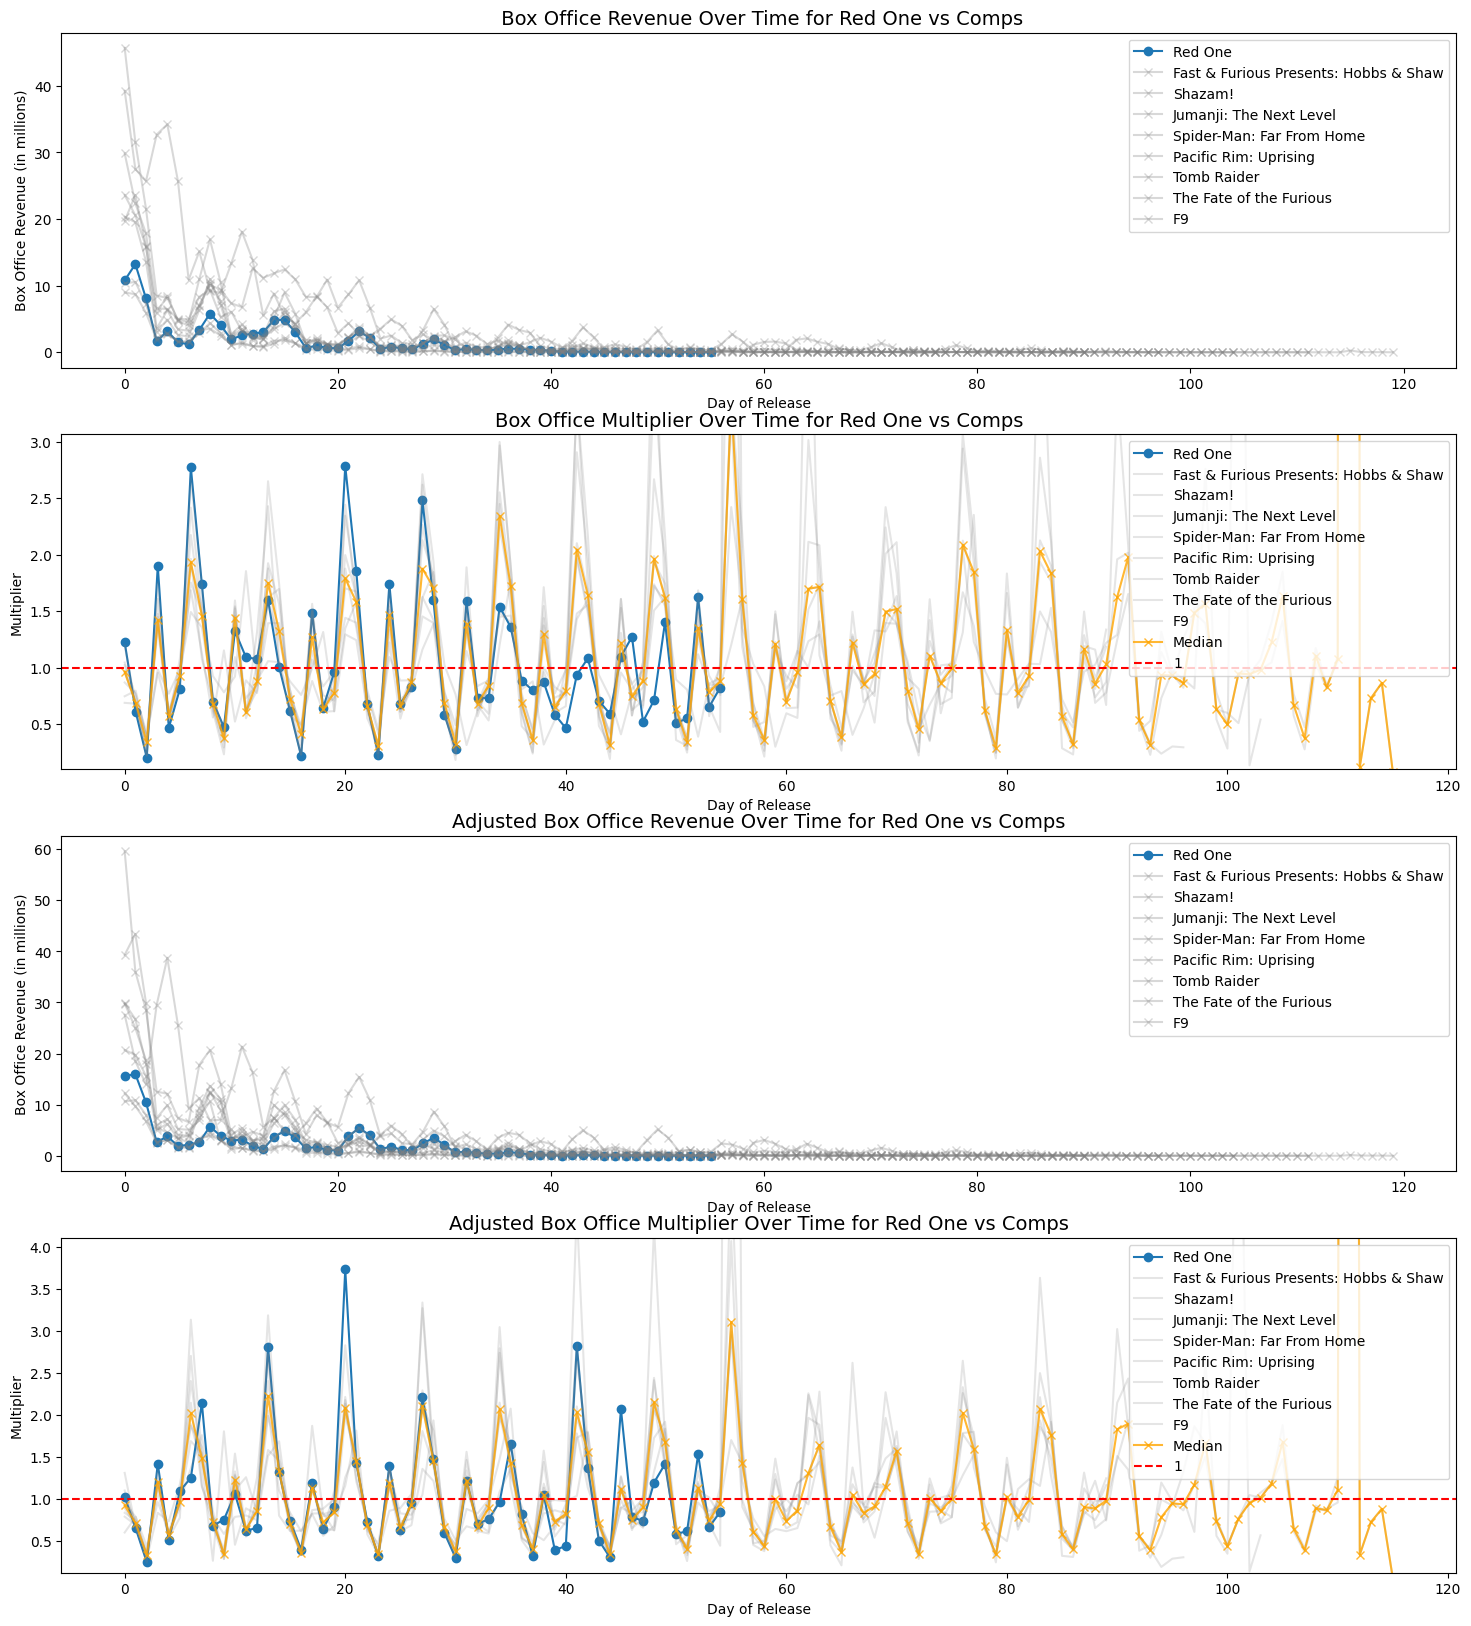
\includegraphics[width=0.8\textwidth]{../shared/images/compsmult/redone.png}
    \caption{This plot shows comps and multipliers for \cite{redOne}. The top plot is box office revenue for Red One and each of its comps; the second plot is multipliers for up to 120 days. The next two plots use adjusted gross instead of raw gross. Adjusted gross is based on seasonal and holiday multipliers.}
    \label{fig:compsmultredone}
\end{figure}

\begin{figure}
    \centering
    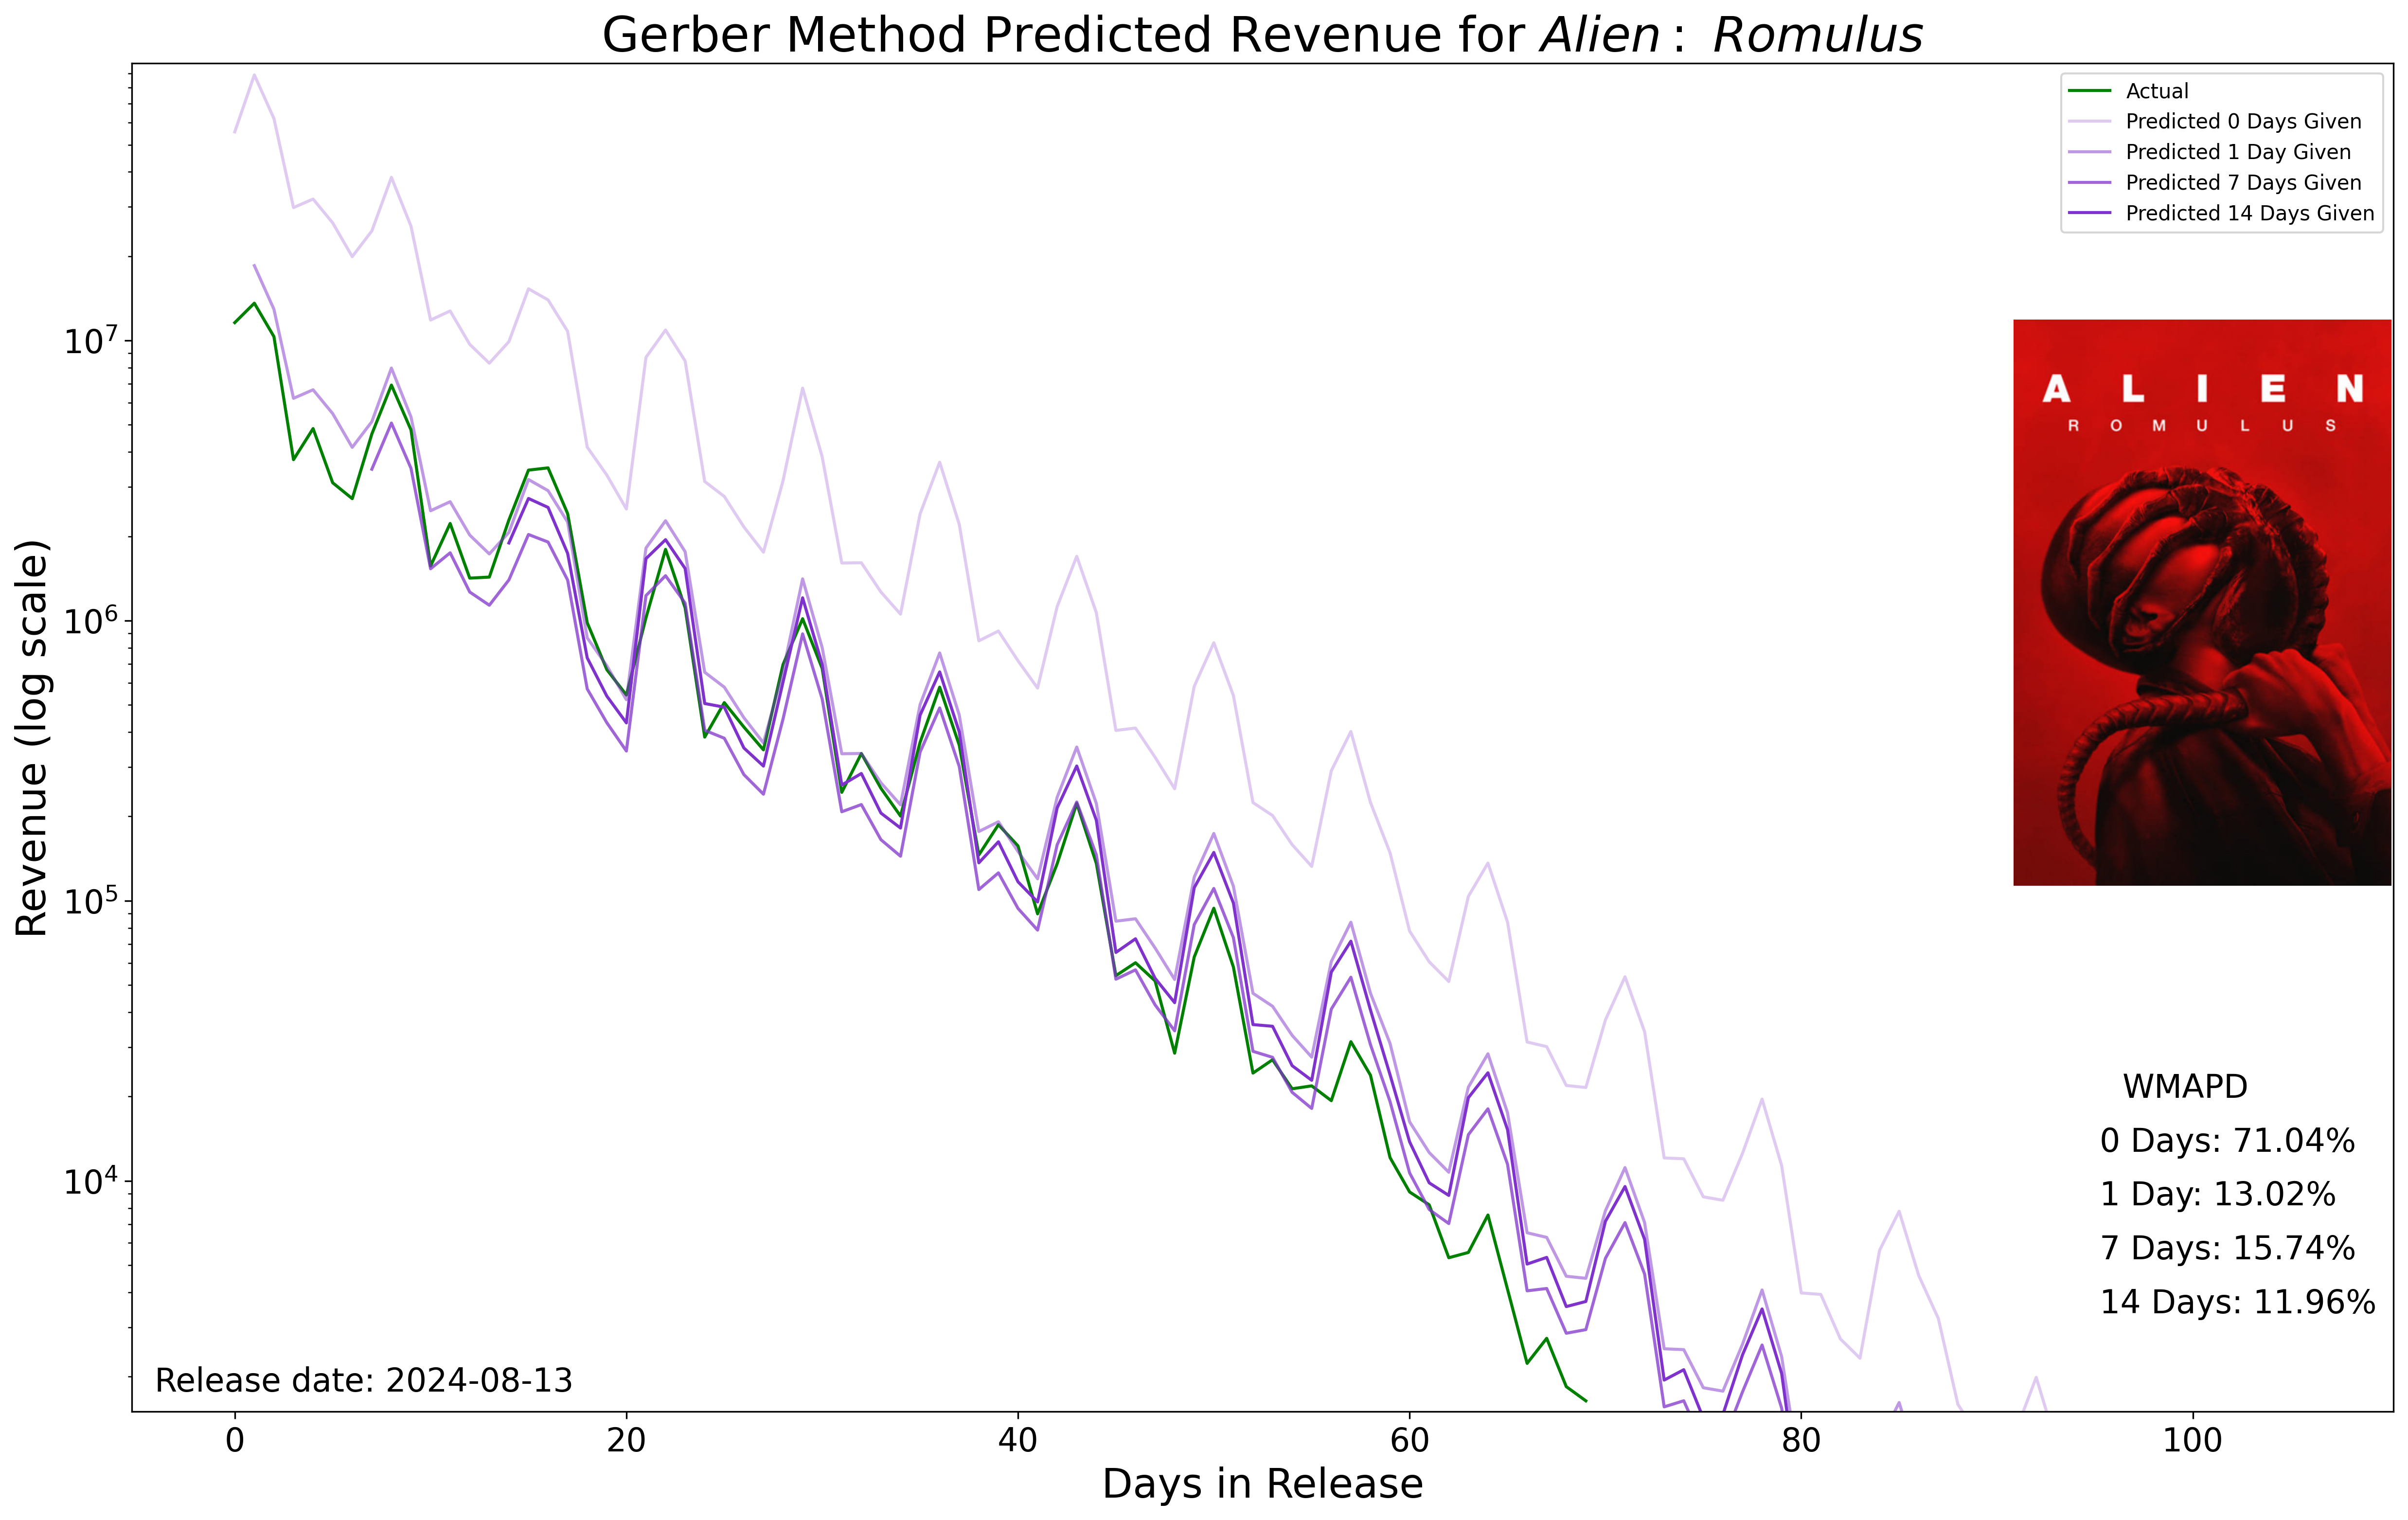
\includegraphics[width=0.9\textwidth]{../shared/images/pred/Alien: Romulus_multiple_4.png}
    \caption{This chart presents predictions for \cite{alienRomulus} given 1 day. The model is quite accurate in general.}
    \label{fig:predalienmulti}
\end{figure}

\begin{figure}
    \centering
    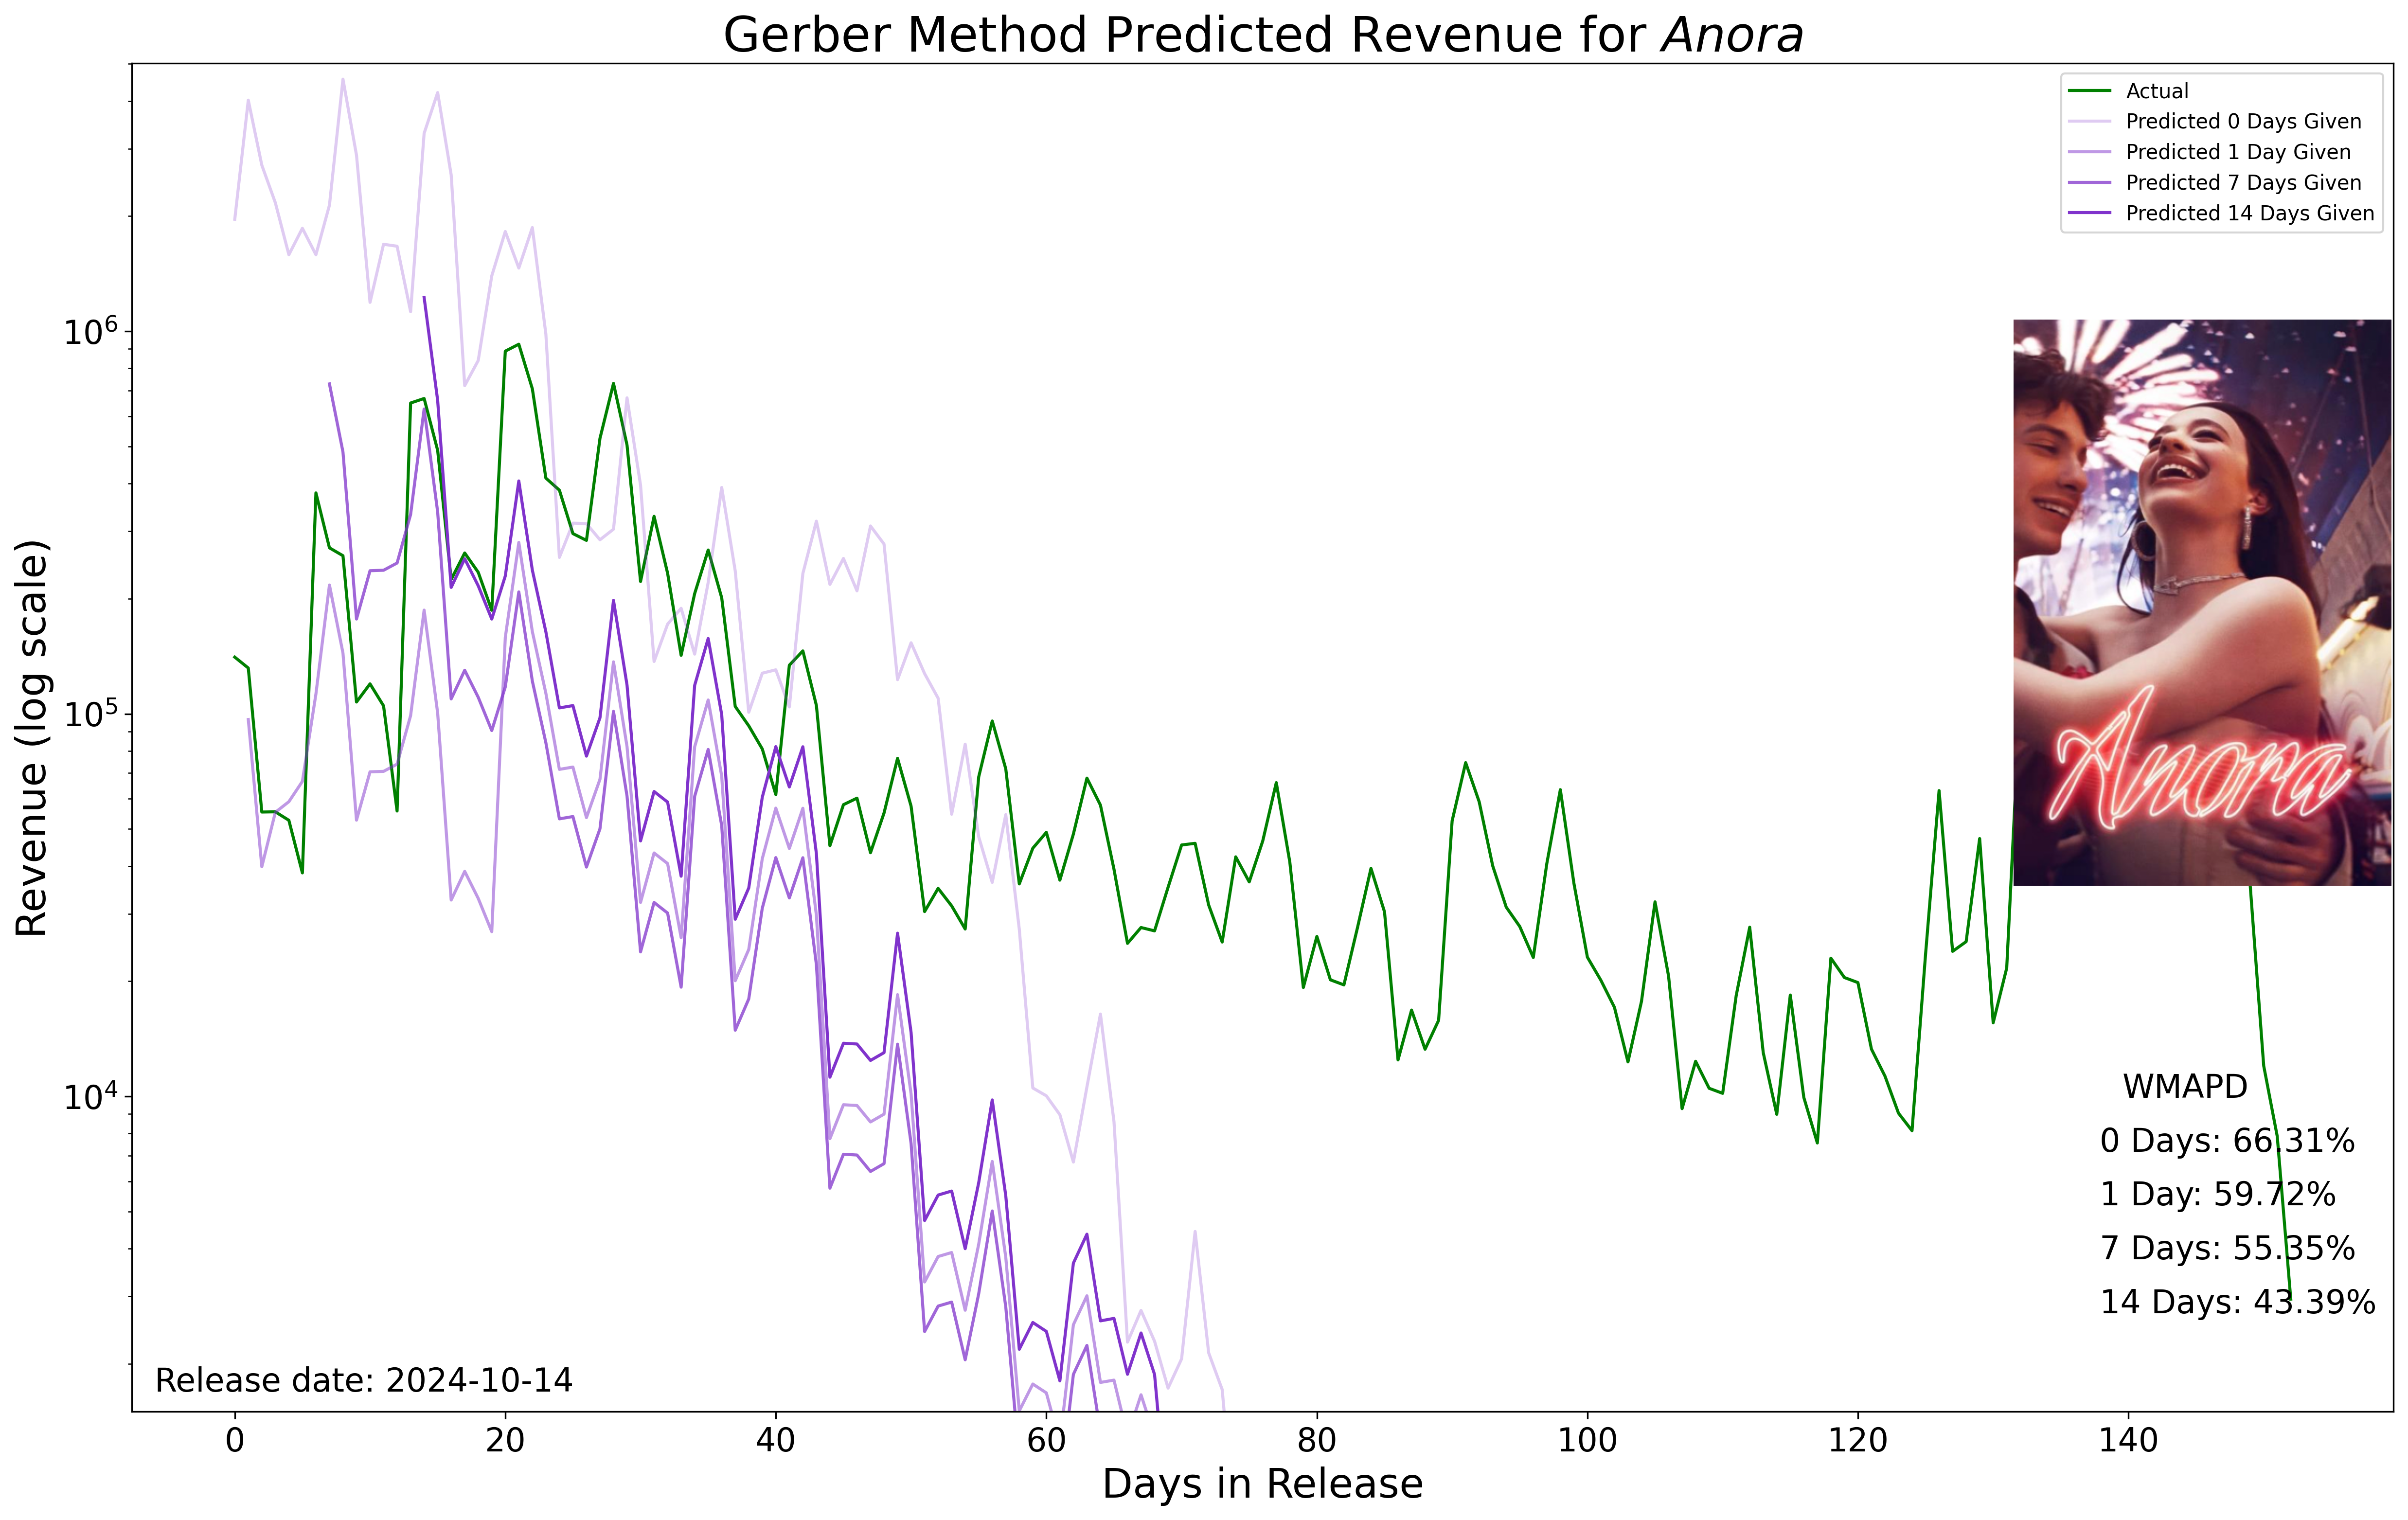
\includegraphics[width=0.9\textwidth]{../shared/images/pred/Anora_multiple_4.png}
    \caption{This chart presents predictions for \cite{anora} given a variety of days. These predictions don't do a great job due to the limited release mentioned in \ref{sec:discussion}.}
    \label{fig:predanora}
\end{figure}

\begin{figure}[H]
    \centering
    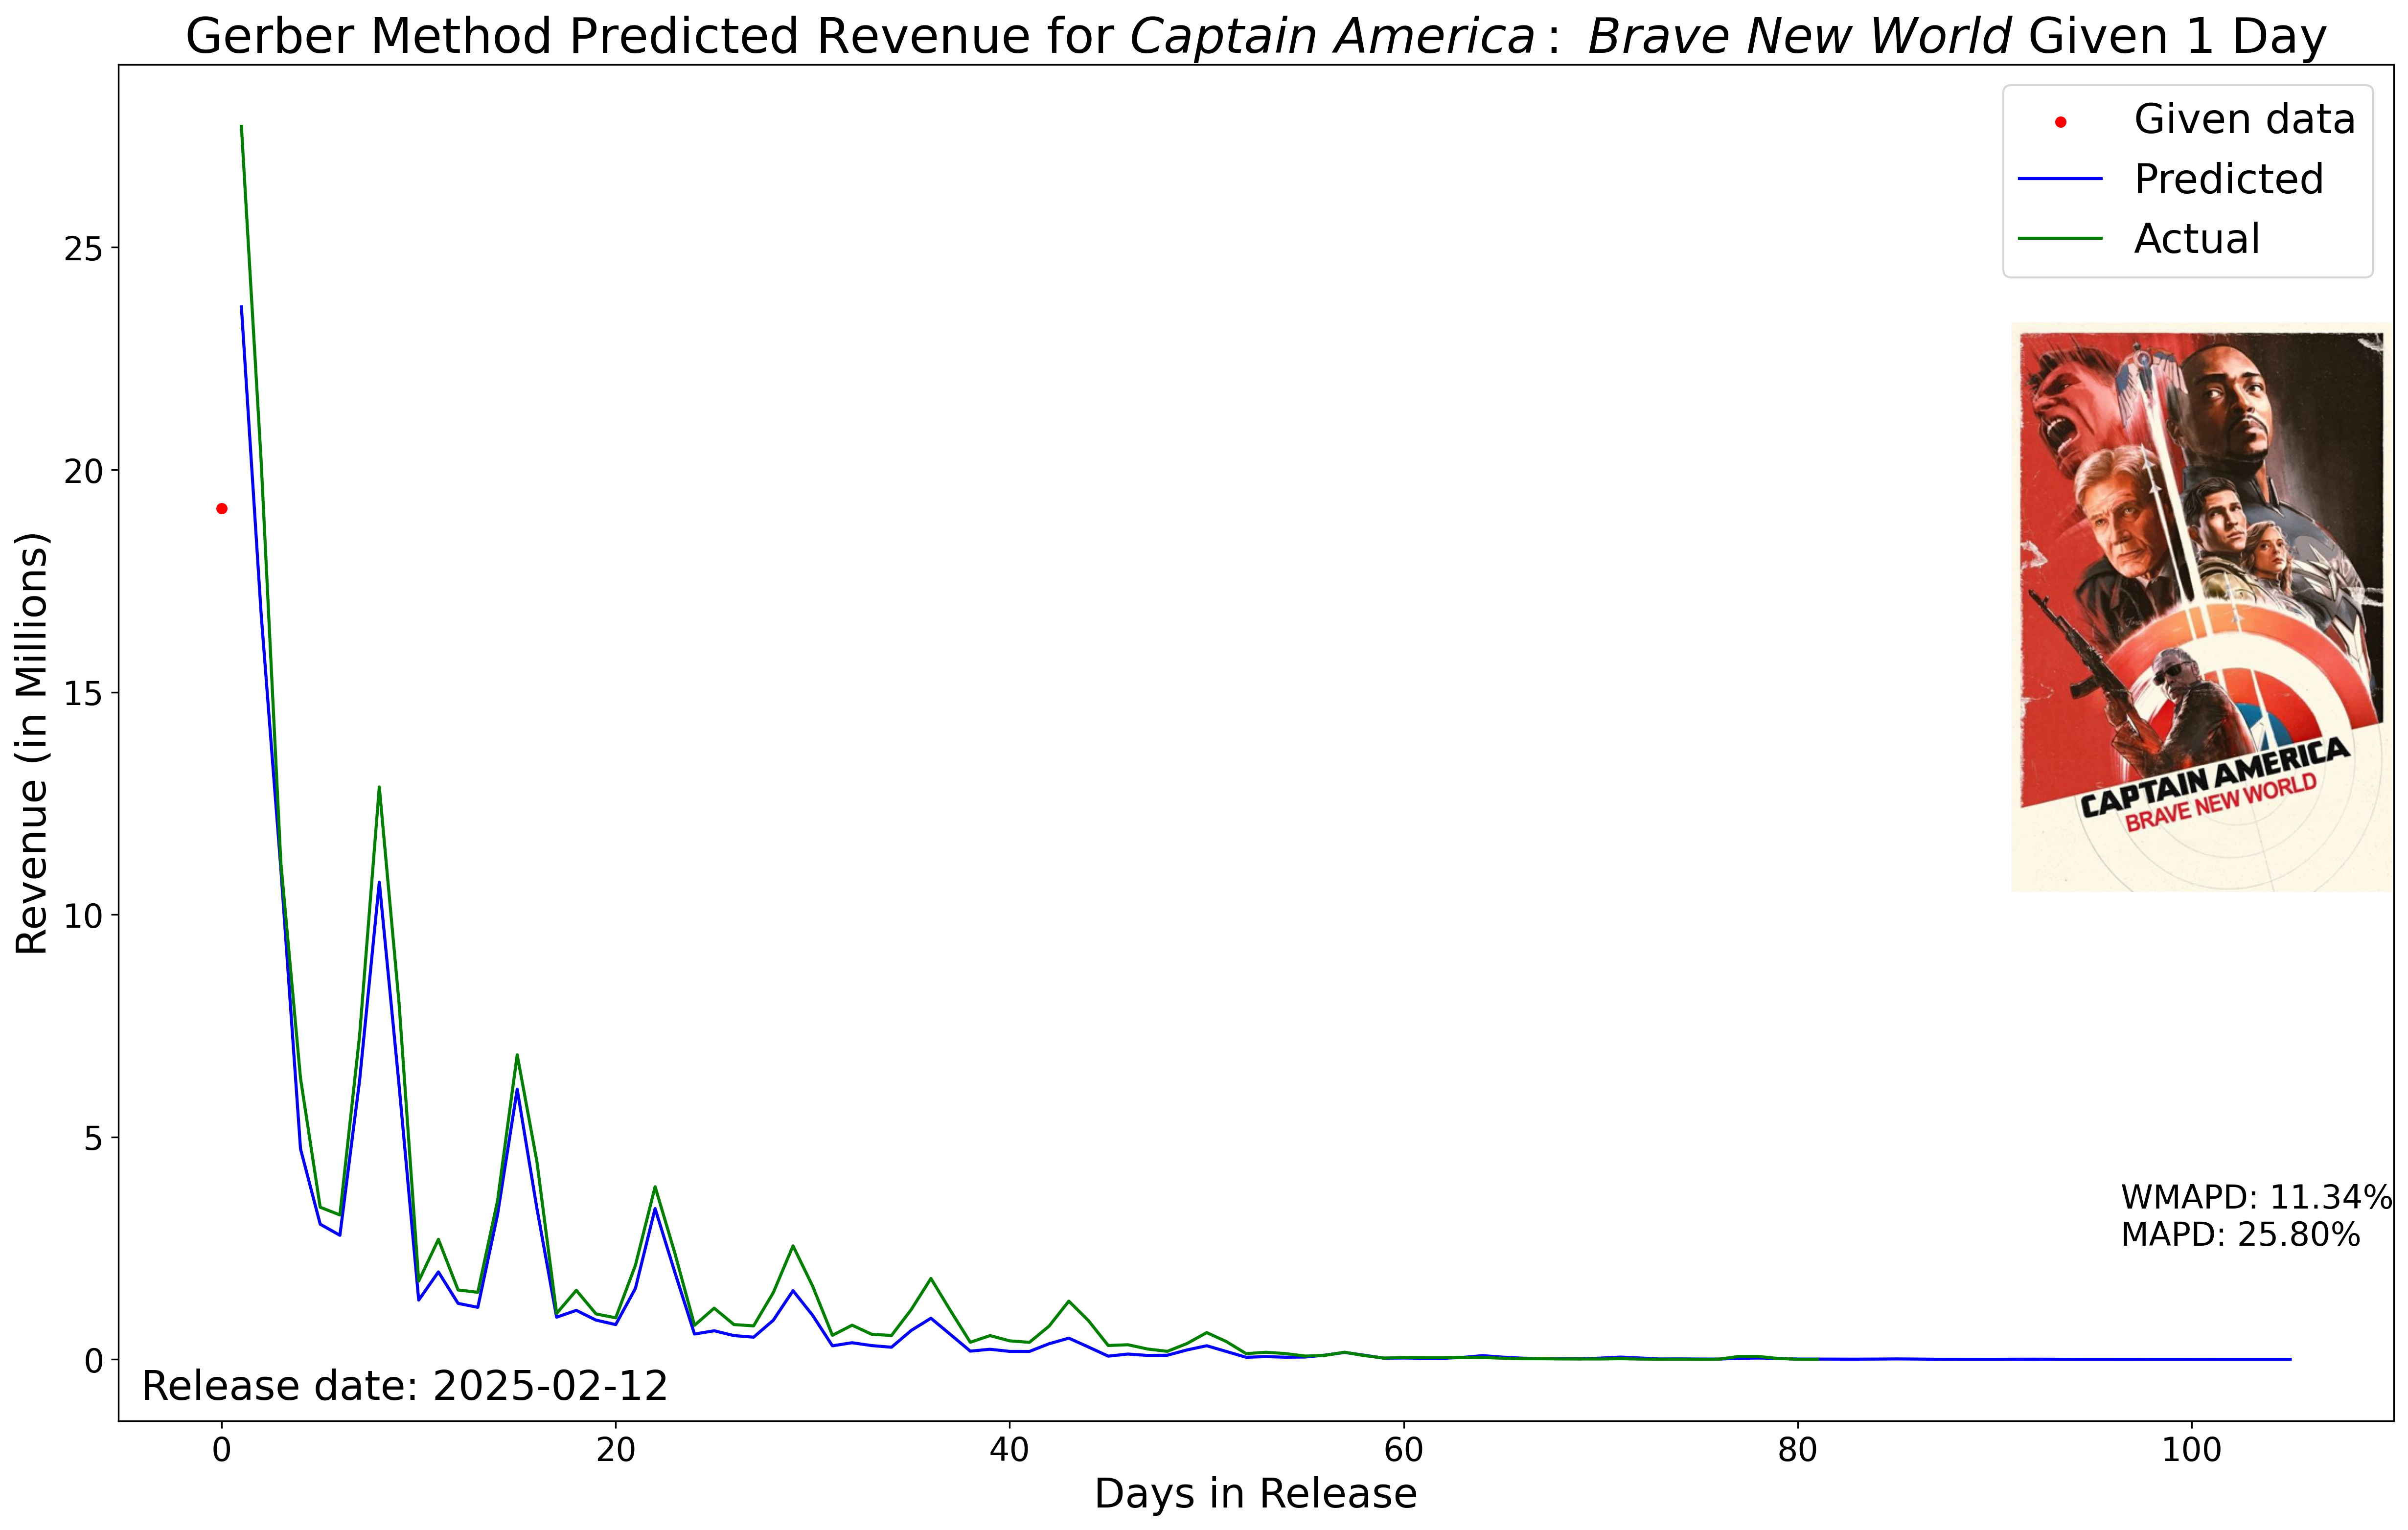
\includegraphics[width=1.0\textwidth]{../shared/images/pred/Captain America: Brave New World_1.png}
    \caption{This plot presents predictions for \cite{captainAmerica} given 1 day.}
    \label{fig:predbrave}
\end{figure}

\begin{figure}
    \centering
    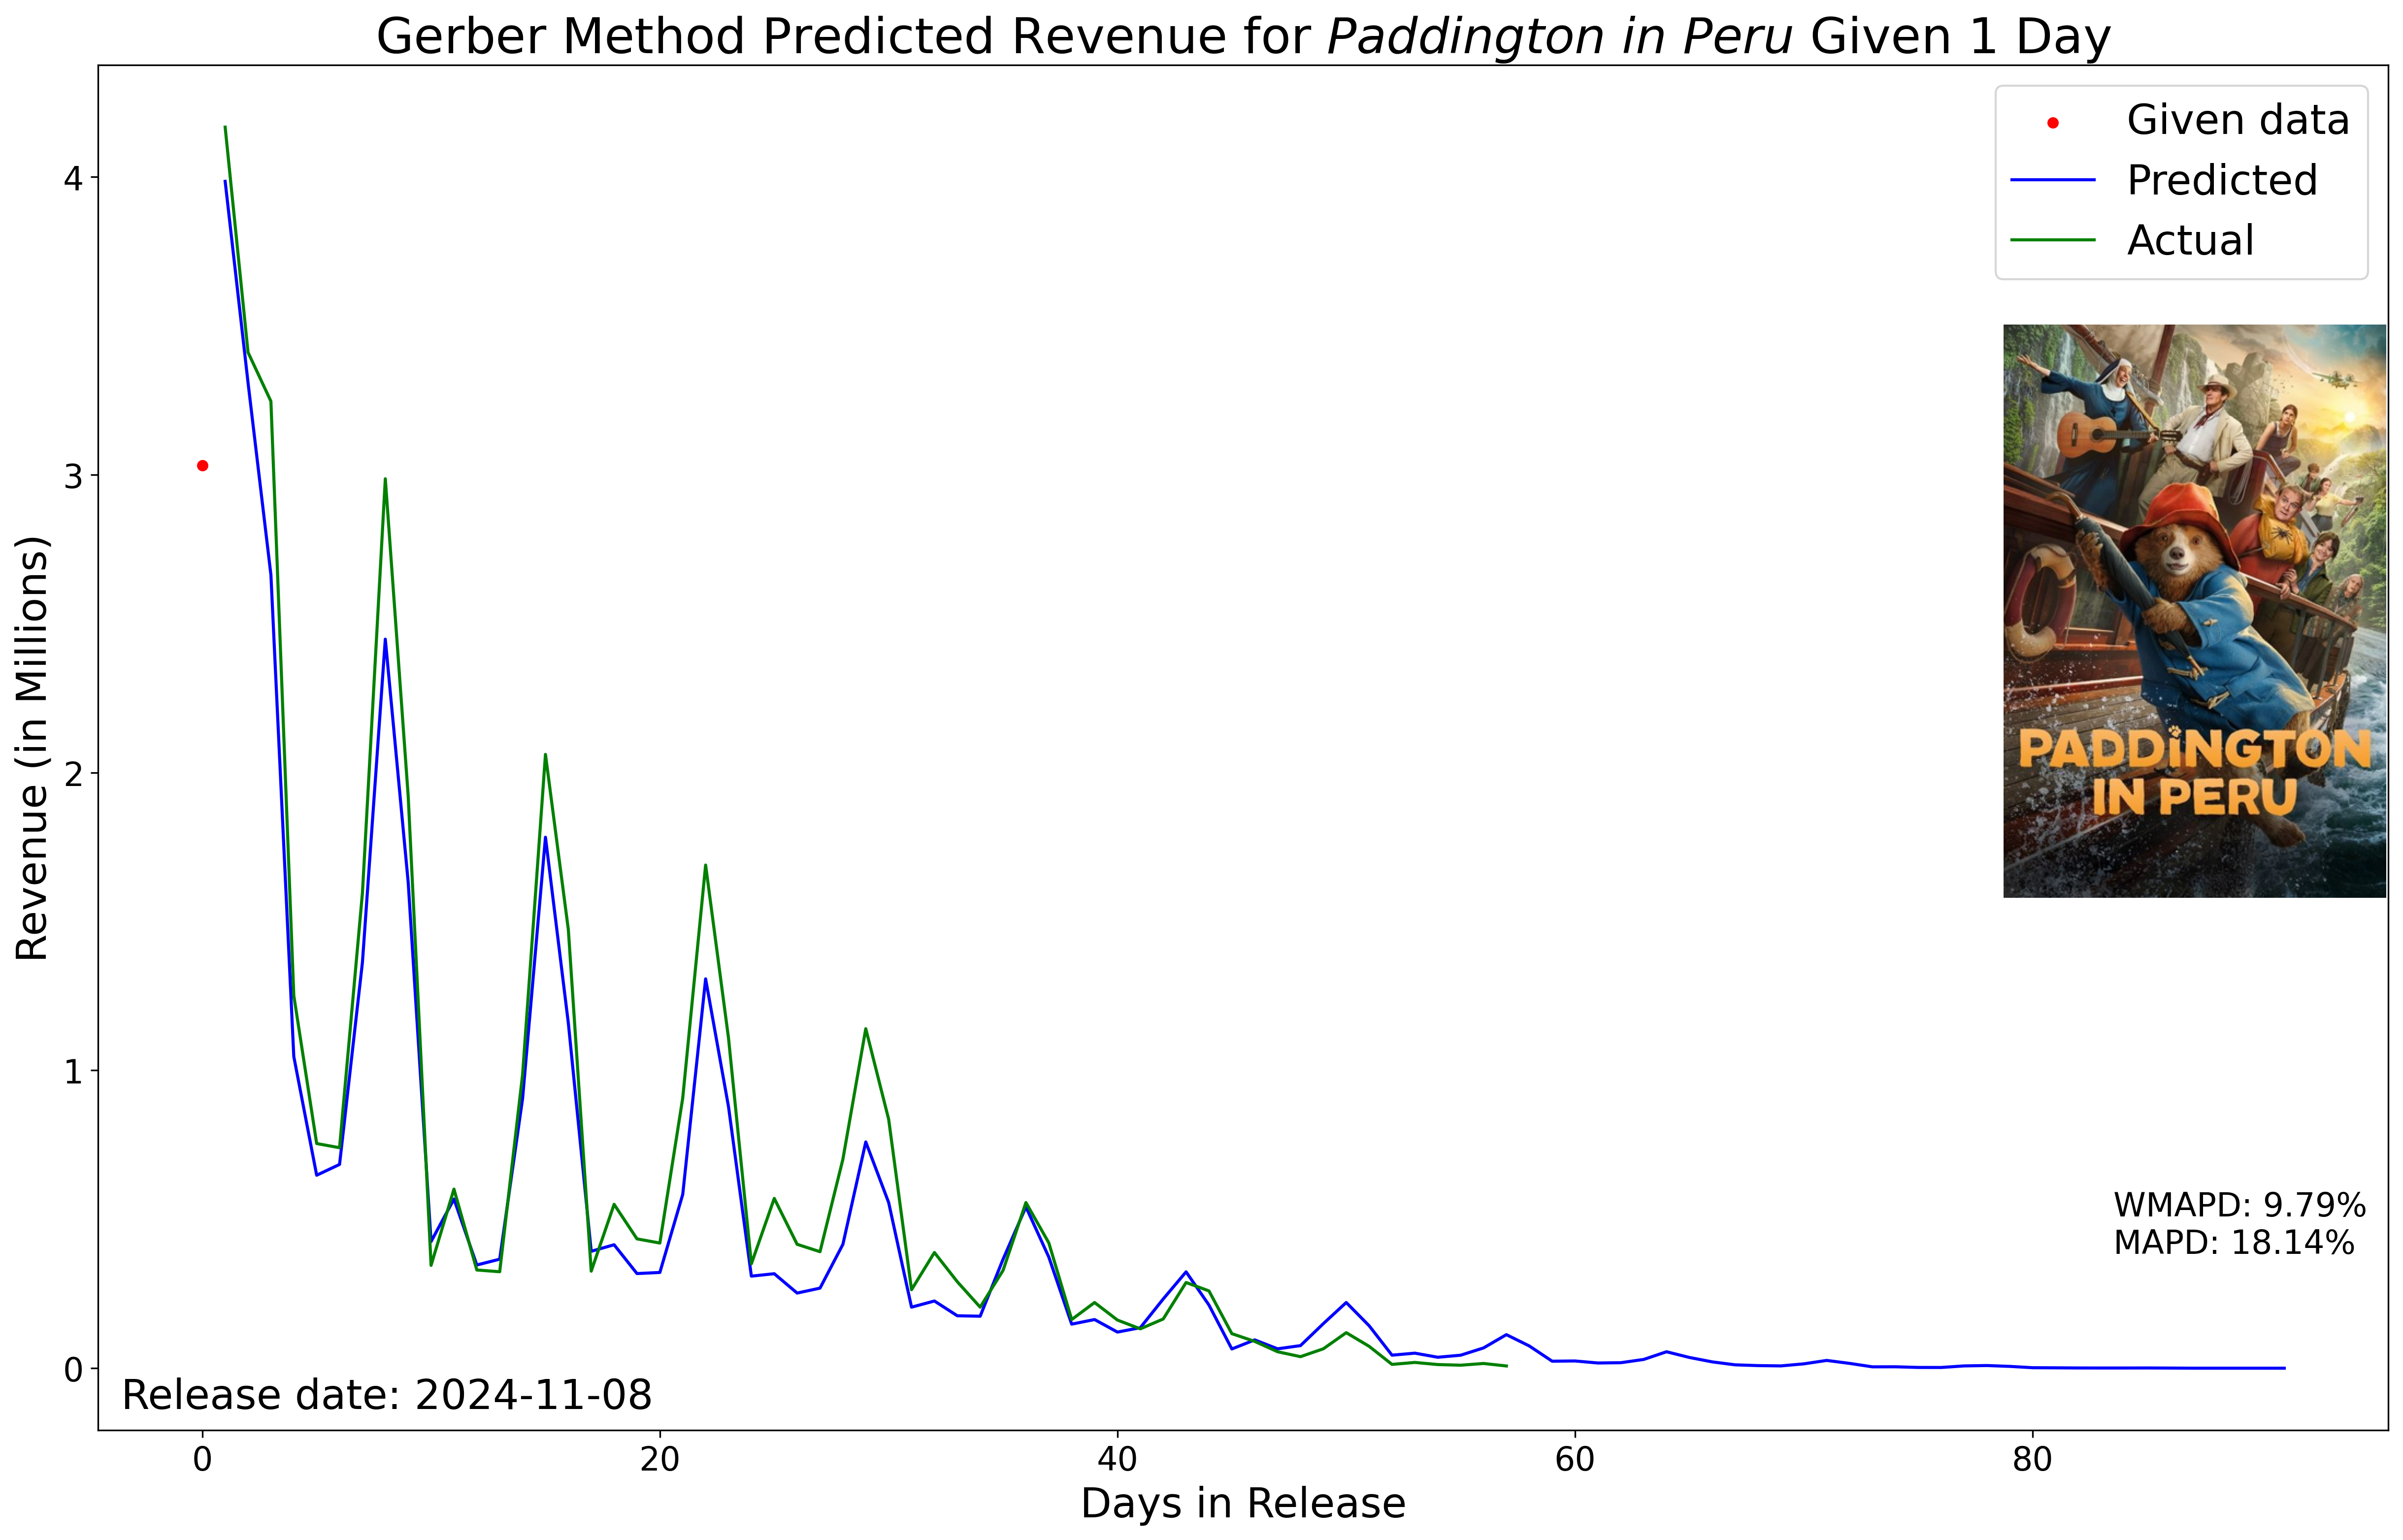
\includegraphics[width=0.9\textwidth]{../shared/images/pred/Paddington in Peru_1.png}
    \caption{This chart presents predictions for \cite{paddingtonPeru} given 1 day. The model is extremely accurate in general.}
    \label{fig:predpaddington}
\end{figure}

\begin{figure}
    \centering
    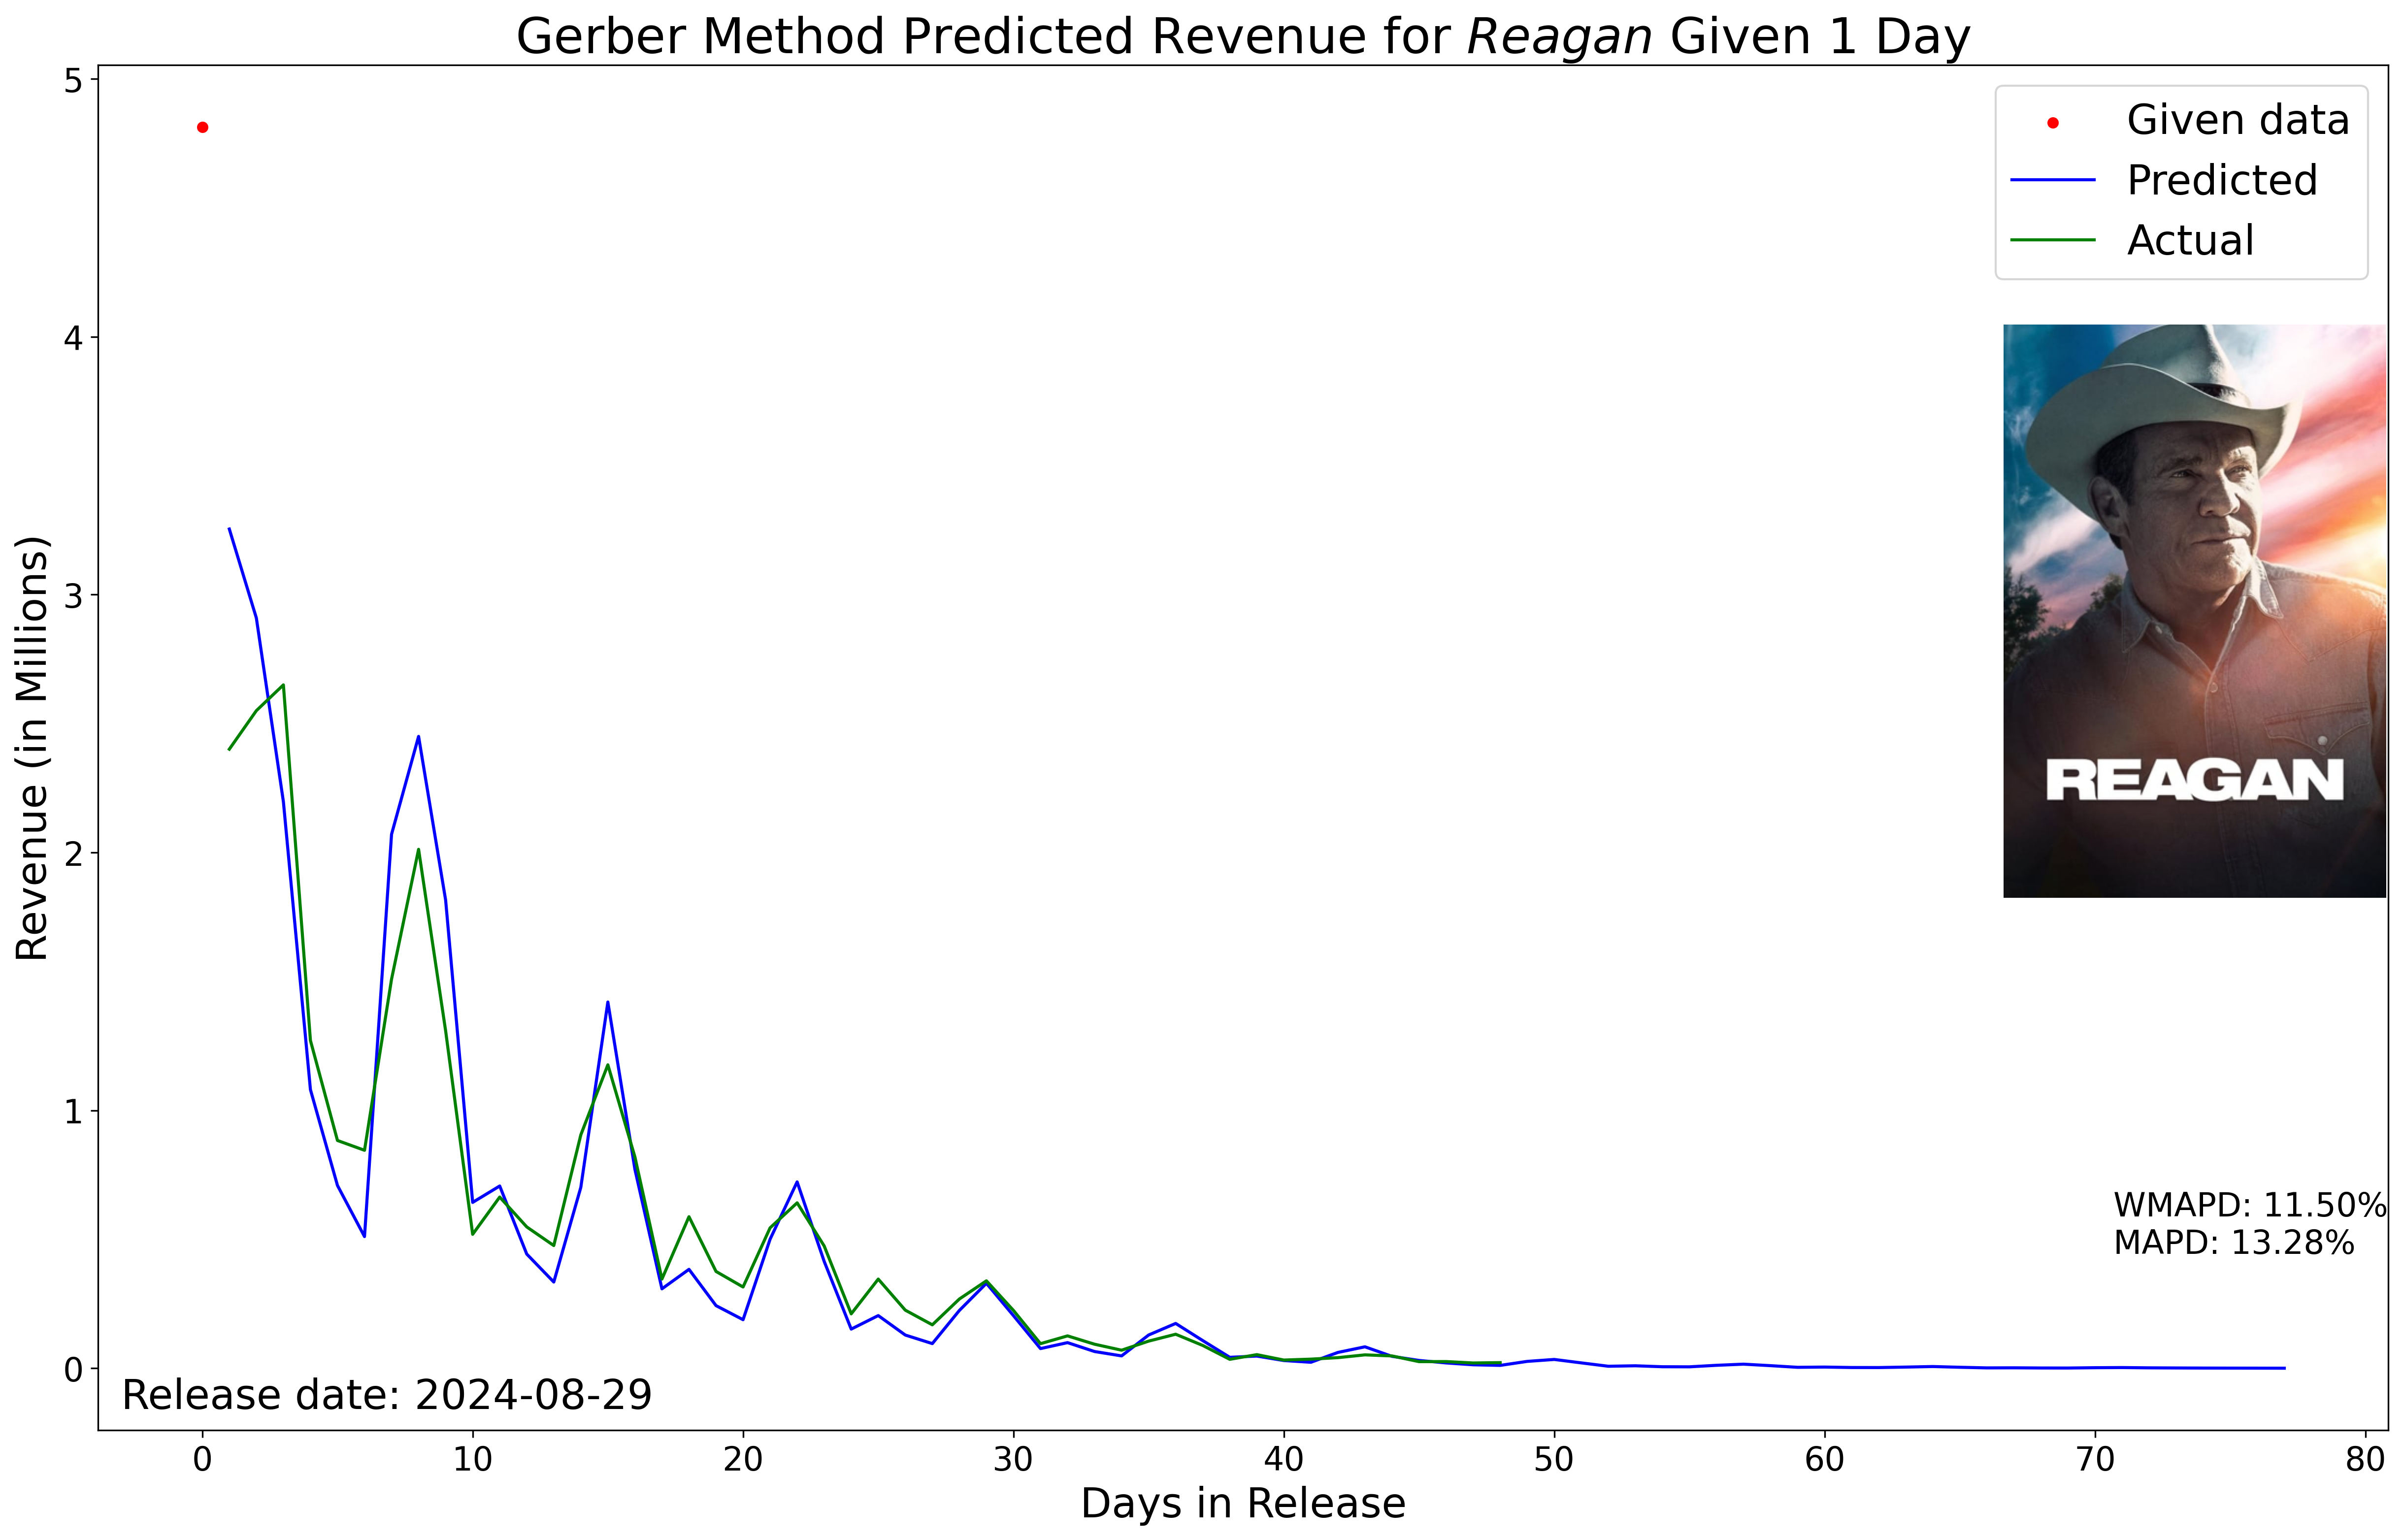
\includegraphics[width=0.9\textwidth]{../shared/images/pred/Reagan_1.png}
    \caption{This chart presents predictions for \cite{reagan} given 1 day. The model is extremely accurate in general.}
    \label{fig:predreagan}
\end{figure}

\begin{figure}
    \centering
    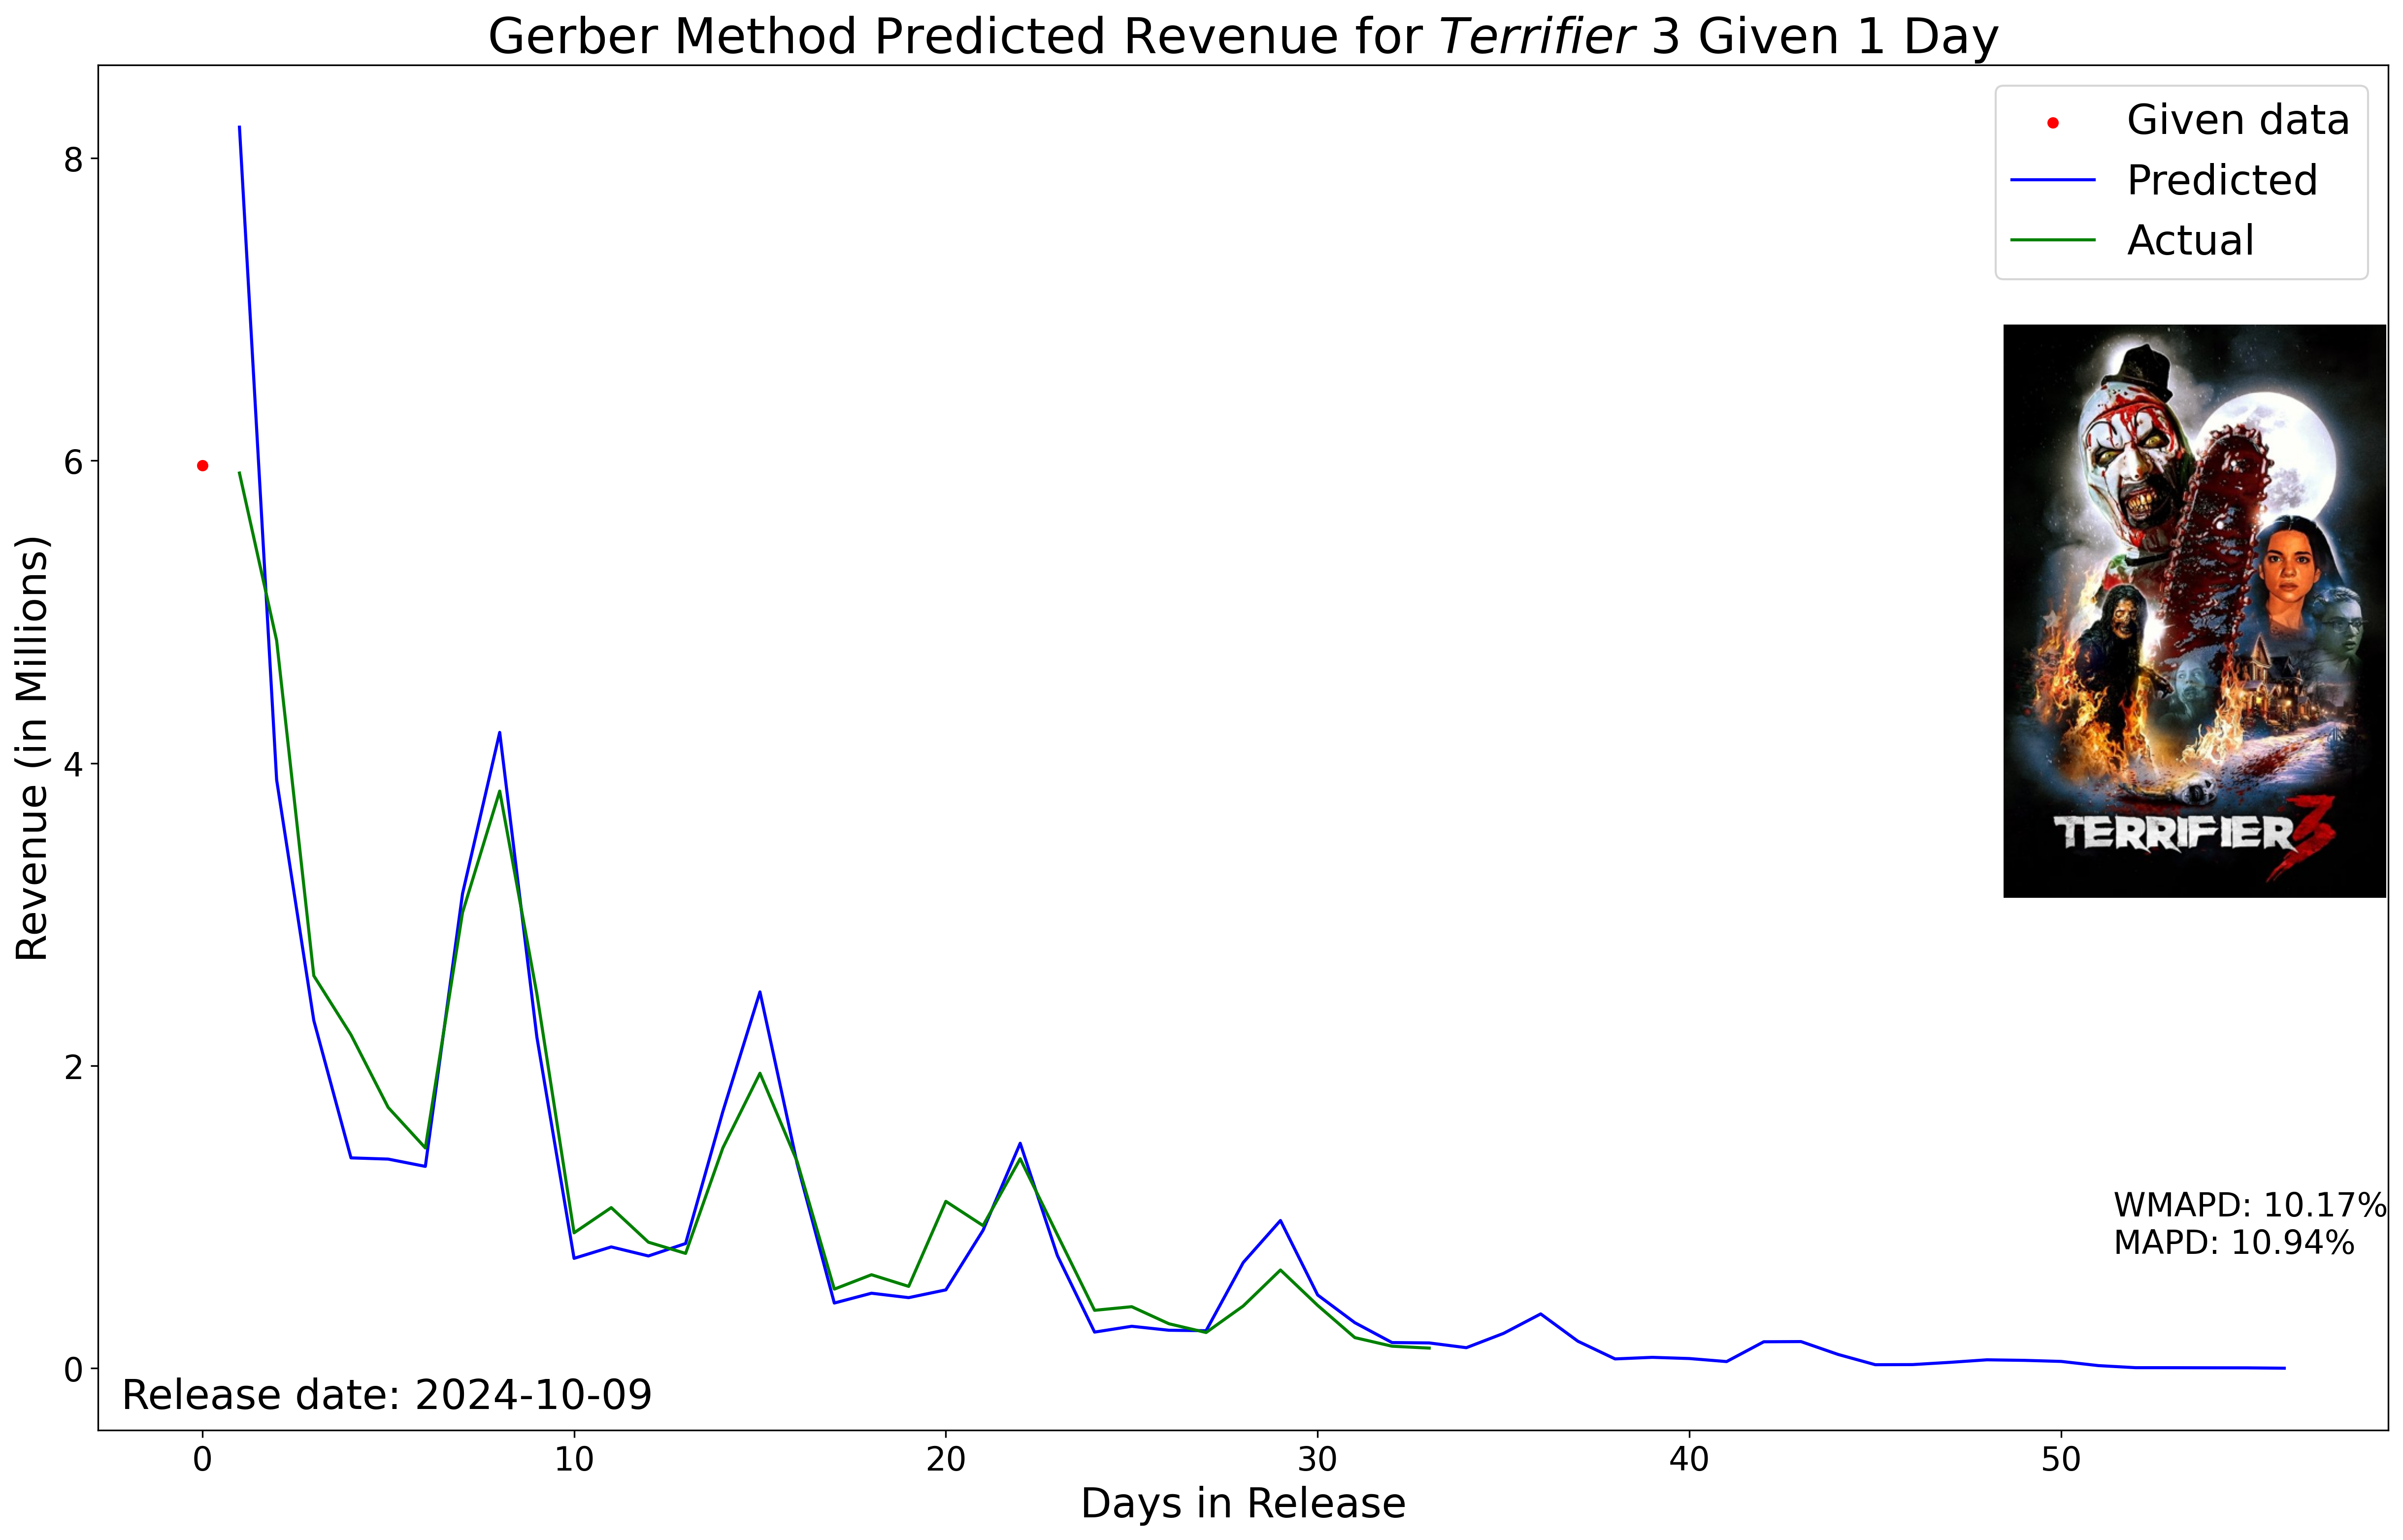
\includegraphics[width=0.9\textwidth]{../shared/images/pred/Terrifier 3_1.png}
    \caption{This chart presents predictions for \cite{terrifier3} given 1 day. The model is quite accurate in general.}
    \label{fig:predterrifier3}
\end{figure}

\begin{figure}[H]
    \centering
    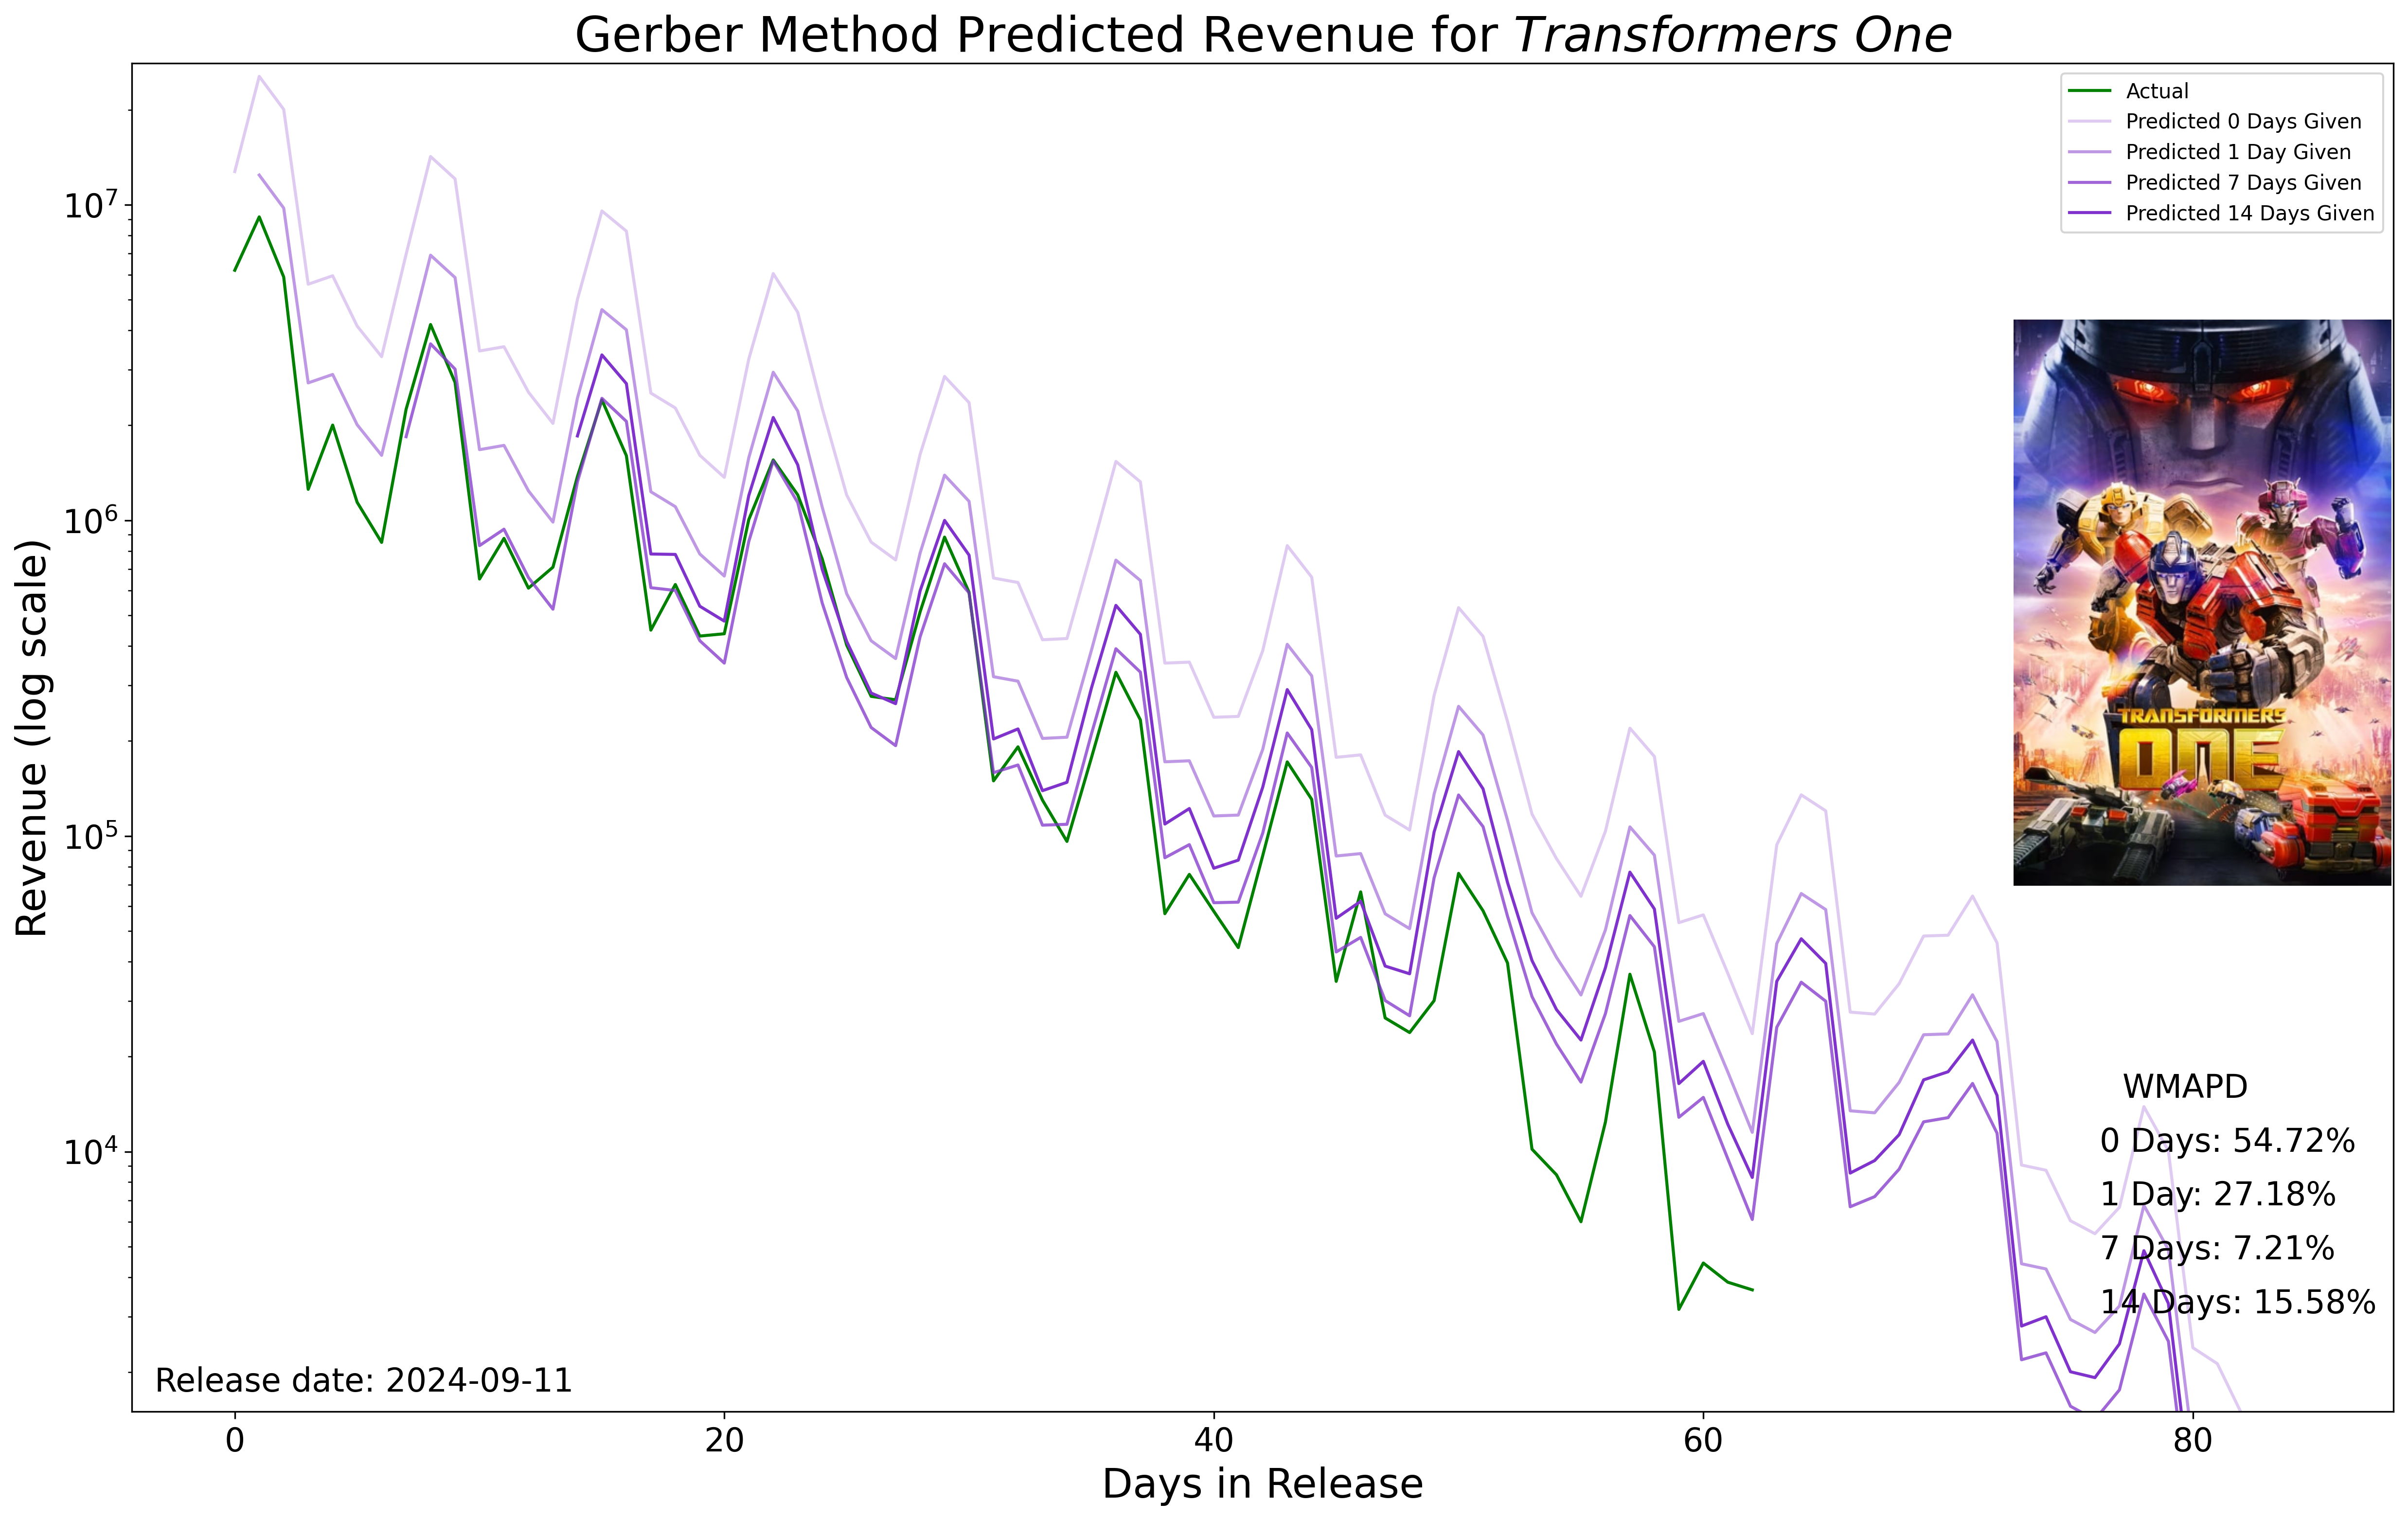
\includegraphics[width=0.9\textwidth]{../shared/images/pred/Transformers One_multiple_4.png}
    \caption{This plot presents predictions for \cite{transformersOne} given 0, 1, 7, and 14 days.}
    \label{fig:predtransformersmulti}
\end{figure}

\begin{figure}
    \centering
    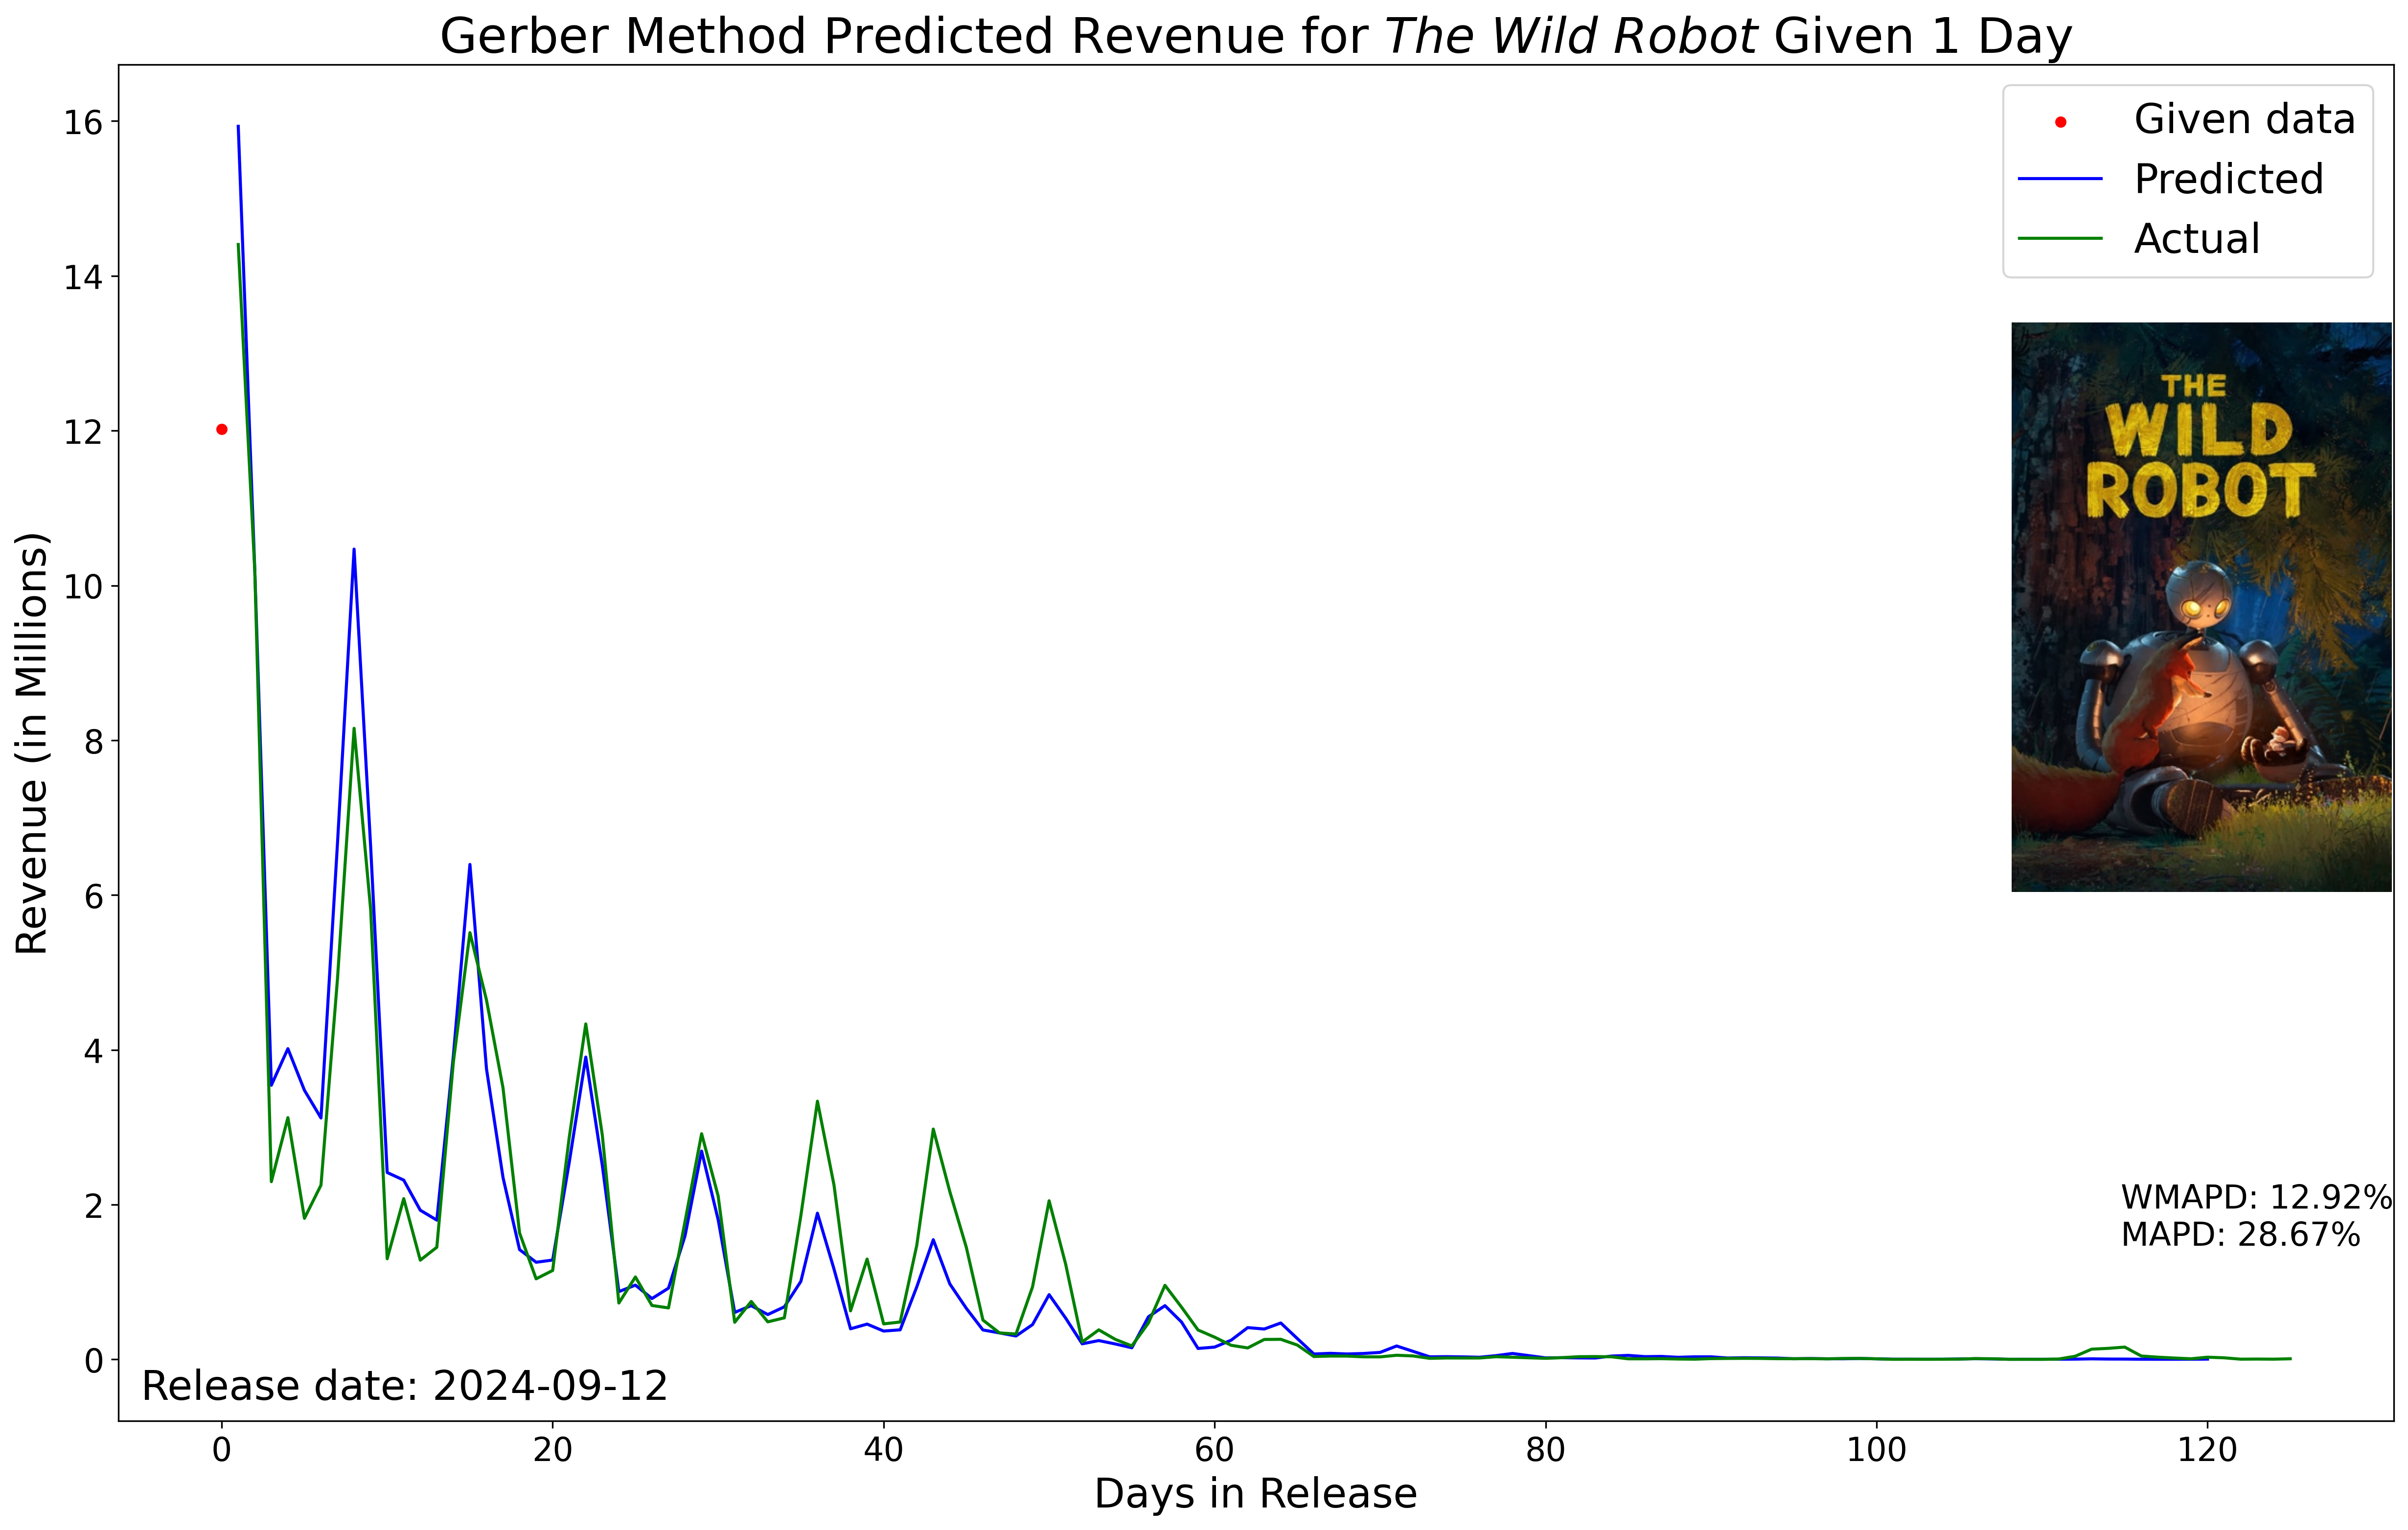
\includegraphics[width=0.9\textwidth]{../shared/images/pred/The Wild Robot_1.png}
    \caption{This chart presents predictions for \cite{wildRobot} given 1 day. The model is quite accurate in general.}
    \label{fig:predwildrobot}
\end{figure}


\end{document}  % --------------------------------------------------------------------------------
